\documentclass[bachelor,german]{hgbthesis}

\usepackage{imakeidx}


\usepackage{hyperref}
\hypersetup{
    hyperindex = true,
    colorlinks=true,
    linkcolor=blue,
    filecolor=magenta,      
    urlcolor=cyan,
}
\makeindex[columns=2, title=Alphabetischer Index, intoc]



%%------------------------------------------------------------

\bibliography{Your bibliography}  

%%--------------------------------------------------------------



%\usepackage{MnSymbol,wasysym}
%\usepackage{comment}
%\usepackage{ulem,nicefrac}
%\usepackage[all]{xy}


\usepackage{graphicx}
\graphicspath{{images/}}

\renewcommand{\labelenumi}{\upshape(\arabic{enumi})}

\usepackage{amssymb}
\usepackage{amsmath}

\usepackage{amsfonts}
%\usepackage{latexsym}
\usepackage{amsthm}
%\usepackage{ifthen}
\usepackage{aliascnt}
\usepackage{cleveref}

\renewcommand\qedsymbol{$\blacksquare$}

\usepackage{titlesec}

\usepackage[left=4.0cm,right=4.0cm,top=1.5cm,bottom=1.5cm,includeheadfoot]{geometry}

\usepackage{mdframed}

\newenvironment{fsatz}
  {\begin{mdframed}\begin{satz}}
  {\end{satz}\end{mdframed}}


\theoremstyle{plain}
\newtheorem{satz}{Satz}[section]

%Neue Umgebungen
\theoremstyle{plain}
\newtheorem{folg}[satz]{Folgerung}
\newtheorem{lem}[satz]{Lemma}
\newtheorem{prop}[satz]{Proposition}
\newtheorem{beh}[satz]{Behauptung}
\newtheorem{axiom}[satz]{Axiom}
\newtheorem{hi}[satz]{Hilfssatz}
\newtheorem{algo}[satz]{Algorithmus}
\newtheorem{aus}[satz]{Aussage}
\newtheorem{theo}[satz]{Theorem}

\theoremstyle{definition}
\newtheorem{defi}[satz]{Definition}
\newtheorem{konstr}[satz]{Konstruktion}
\newtheorem{verein}[satz]{Vereinbarung}
\newtheorem{bem}[satz]{Bemerkung}
\newtheorem{bsp}[satz]{Beispiel}
\newtheorem{mem}[satz]{Erinnerung}
\newtheorem{aufg}[satz]{Aufgabe}
\newtheorem{probl}[satz]{Problemstellung}
\newtheorem{moti}[satz]{Motivation}

\renewcommand*{\proofname}{Beweis}

%\usepackage{mathtools}

% \usepackage{imakeidx}

% \makeindex[columns=3, title=Alphabetical Index]

\usepackage{soulutf8}

\numberwithin{equation}{satz}


%%%----------------------------------------------------------
\begin{document}
%%%----------------------------------------------------------

% Einträge für ALLE Arbeiten: --------------------------------
\title{Über positive Störungen auf Kantorovich-Banachräumen}
\author{Jörg Schwartz}
\studiengang{Mathematik}
\studienort{\textsc{Eberhard Karls Universität Tübingen}}
\abgabedatum{2017}{09}{11}	% {YYYY}{MM}{DD}

%%% zusätzlich für eine Bachelorarbeit: ---------------------
\nummer{3610471}   % XX...X = Stud-ID, z.B. 0310238045-A  
                        % (A = 1. Bachelorarbeit)
\semester{Sommersemester 2017} 
\gegenstand{zur Operatorentheorie} 
\betreuer{Prof. Dr. Rainer Nagel} % oder \betreuerin{..}

%%%----------------------------------------------------------
\frontmatter
\maketitle
\tableofcontents

%%%----------------------------------------------------------

% \chapter{Kurzfassung}

\par
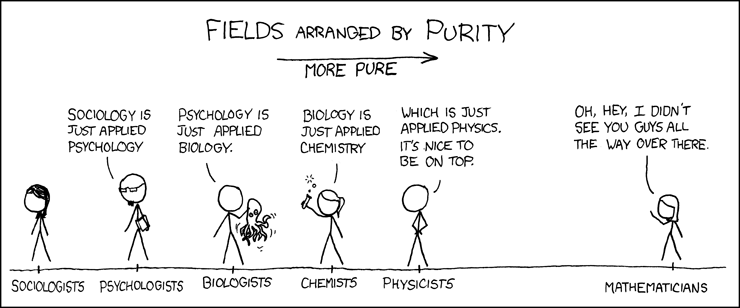
\includegraphics[scale = 0.46]{purity}

\par
\textbf{Problem}: Sei $(A, D(A))$ Generator einer $C_0$-Halbgruppe auf einem Banachraum $X$ und $(B, D(B))$ ein weiterer Operator auf $X$. Unter welchen Bedingungen ist $A+B$, oder eine Fortsetzung $K$ von $A+B$, Generator einer $C_0$ Halbgruppe auf $X$?

\par
% 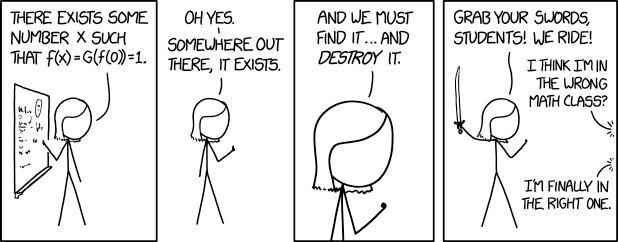
\includegraphics[scale = 0.55]{existence_proof}

% An dieser Stelle steht eine Zusammenfassung der Arbeit, Umfang
% max.\ 1 Seite. Im Unterschied zu anderen Kapiteln ist die
% Kurzfassung (und das Abstract) üblicherweise nicht in Abschnitte
% und Unterabschnitte gegliedert. 
% Auch Fußnoten sind hier falsch am Platz.

% Kurzfassungen werden übrigens häufig -- zusammen mit Autor und Titel
% der Arbeit -- %
% in Literaturdatenbanken aufgenommen. Es ist daher darauf zu
% achten, dass die Information in der Kurzfassung für sich 
% \emph{allein} (\dah ohne weitere Teile der Arbeit) zusammenhängend und
% abgeschlossen ist. Insbesondere werden an dieser Stelle (wie \ua
% auch im \emph{Titel} der Arbeit und im \emph{Abstract})
% normalerweise \emph{keine Literaturverweise} verwendet! Falls man
% unbedingt solche benötigt -- etwa weil die Arbeit eine
% Weiterentwicklung einer bestimmten, früheren Arbeit darstellt --,
% dann sind \emph{vollständige} Quellenangaben in der Kurzfassung
% selbst notwendig, \zB %
% [\textsc{Zobel} J.: \textit{Writing for Computer Science -- The Art of
% Effective Commu\-nica\-tion}. Springer-Verlag, Singa\-pur, 1997].

% Weiters sollte man daran denken, dass bei der Aufnahme in Datenbanken
% Sonderzeichen oder etwa Aufzählungen mit "`Knödellisten"' in der
% Regel verloren gehen. Dasselbe gilt natürlich auch für das 
% \emph{Abstract}.


% Inhaltlich sollte die Kurzfassung \emph{keine} Auflistung der
% einzelnen Kapitel sein (dafür ist das Einleitungskapitel
% vorgesehen), sondern dem Leser einen kompakten, inhaltlichen
% Überblick über die gesamte Arbeit verschaffen. Der hier verwendete
% Aufbau ist daher zwangsläufig anders als der in der Einleitung.
		

%%%----------------------------------------------------------
\mainmatter         % Hauptteil (ab hier arab. Seitenzahlen)
%%%----------------------------------------------------------
% \chapter{Kurzfassung}

\par
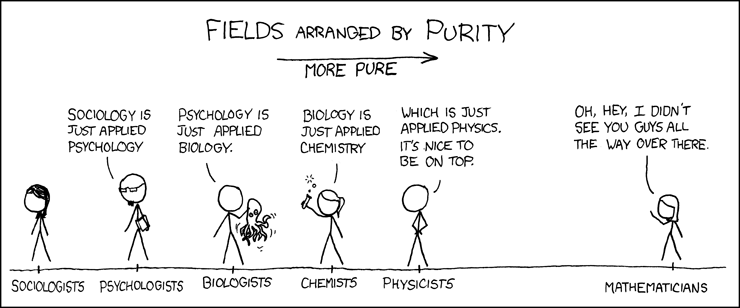
\includegraphics[scale = 0.46]{purity}

\par
\textbf{Problem}: Sei $(A, D(A))$ Generator einer $C_0$-Halbgruppe auf einem Banachraum $X$ und $(B, D(B))$ ein weiterer Operator auf $X$. Unter welchen Bedingungen ist $A+B$, oder eine Fortsetzung $K$ von $A+B$, Generator einer $C_0$ Halbgruppe auf $X$?

\par
% 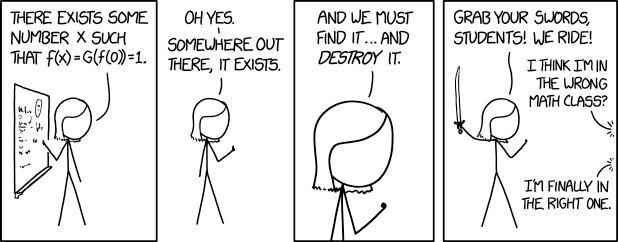
\includegraphics[scale = 0.55]{existence_proof}

% An dieser Stelle steht eine Zusammenfassung der Arbeit, Umfang
% max.\ 1 Seite. Im Unterschied zu anderen Kapiteln ist die
% Kurzfassung (und das Abstract) üblicherweise nicht in Abschnitte
% und Unterabschnitte gegliedert. 
% Auch Fußnoten sind hier falsch am Platz.

% Kurzfassungen werden übrigens häufig -- zusammen mit Autor und Titel
% der Arbeit -- %
% in Literaturdatenbanken aufgenommen. Es ist daher darauf zu
% achten, dass die Information in der Kurzfassung für sich 
% \emph{allein} (\dah ohne weitere Teile der Arbeit) zusammenhängend und
% abgeschlossen ist. Insbesondere werden an dieser Stelle (wie \ua
% auch im \emph{Titel} der Arbeit und im \emph{Abstract})
% normalerweise \emph{keine Literaturverweise} verwendet! Falls man
% unbedingt solche benötigt -- etwa weil die Arbeit eine
% Weiterentwicklung einer bestimmten, früheren Arbeit darstellt --,
% dann sind \emph{vollständige} Quellenangaben in der Kurzfassung
% selbst notwendig, \zB %
% [\textsc{Zobel} J.: \textit{Writing for Computer Science -- The Art of
% Effective Commu\-nica\-tion}. Springer-Verlag, Singa\-pur, 1997].

% Weiters sollte man daran denken, dass bei der Aufnahme in Datenbanken
% Sonderzeichen oder etwa Aufzählungen mit "`Knödellisten"' in der
% Regel verloren gehen. Dasselbe gilt natürlich auch für das 
% \emph{Abstract}.


% Inhaltlich sollte die Kurzfassung \emph{keine} Auflistung der
% einzelnen Kapitel sein (dafür ist das Einleitungskapitel
% vorgesehen), sondern dem Leser einen kompakten, inhaltlichen
% Überblick über die gesamte Arbeit verschaffen. Der hier verwendete
% Aufbau ist daher zwangsläufig anders als der in der Einleitung.
	
\chapter{Motivation}

\section{Geburts- und Todesprozesse (GTP)}

\par
Wir wollen mithilfe eines \textbf{Geburts- und Todesprozess} (GTP), der Spezialfall eines \textbf{Kolmogorov'schen Differentialsystem}, die Entwicklung einer Population in Abhängigkeit der Zeit beschreiben. Dieses abzählbare System an Elementen ist gegeben durch
\begin{align*}
x_0' &= -a_0x_0 + d_1 x_1\\
&\;\;\vdots\\
x_n' &= -a_nx_n + d_{n+1}x_{n+1} + b_{n-1}x_{n-1}  \\
&\;\;\vdots
\end{align*}

\par 
In diesem Falle ist bezeichnet $x_n$ die \textbf{Wahrscheinlichkeit}, mit der die Population zu einem gewissen Zeitpunkt $t$ aus $n$ Individuen besteht. Mithilfe eines (nicht spezifizierten) Mechanismus kann sich der Zustand des Systems zu $k+1$, vermöge der 'Geburt' eines Individuums, oder analog zu $k-1$, vermöge des 'Todes' eines Individuums, ändern; bezeichnen die Wahrscheinlichkeit, mit der eine Zustandsänderung $k\mapsto k+1$ auftritt mit  $b_k$ und analog $d_k$ für $k\mapsto k-1$; mit $a_n=d_n+b_n$ bezeichnet man obiges System auch als klassischen GTP.

In \cite{kato_1954} zeigt Kato die Existenz einer $C_0$-Halbgruppe, welche obiges Kolmogorov'sche Differentialsystem für alle absolut summierbaren Folgen $\textbf{x}\in l_1$ löst. Das Ergebnis wurde  in \cite{} auf AL-Räume verallgemeinert, welche die Räume $l_1$ und $L_1$ umfassen. In diesem Text stellen wir das Ergebnis von Banasiak et al.  \cite{banasiak_lachowicz_2007} vor, welches die Existenz für Operatoren in KB-Räumen verallgemeinert. Diese umfassen neben den AL-Räumen auch reflexive Banachräume. 





% Jedoch, falls wir die Existenz einer Halbgruppe beweisen, welche \Cref{} "löst", dann ist das, was wir wirklich erhalten, ist eine Lösung zu einer bestimmten Reformulierung des ursprünglichen Problems in welchem auf der rechten Sete steht der Genrator $K$ einer Halbgruppe. Dieser Generator kann sehr verschieden von $\mathcal A+\mathcal b$ sein und nur eine detailierte Charakterisierung von seinem Definitionsbereich  kann enthüllen ob  die konstruierte Halbgruppe gibt das volle Bild der dynamik beschreiben bei Gleichung \Cref{}. Wie wir zeigen, der Generator $K$ ist zwischen dem minimalen Operator $K_{min}=A+B$ definiert auf $D(A)$ und dem maximalen Operator $K_{max}=\mathcal A+\mathcal b$ definiert auf
% \begin{equation*}
% D_{max}=\{\textbf{u}\in X;\mathcal A\textbf{u}+ \mathcal B\textbf{u}\in X\};
% \end{equation*}
% das heißt also $K_{min}\subseteq K\subseteq K_{max}$. Wo $K$ ist situiert auf einer Skala bestimmt die wohl-gestelltheit des Problems von \Cref{}. Die folgenden Situation sind möglich
% \begin{enumerate}
% \item
% \item
% \end{enumerate}
% und jede dieser hat seine eigene spezifische Interpretation in dem Model.

% \par
% In jedem Falle wo $K\subsetneq K_{max}$ ist keine Eindeutigkeit; das heißt, es gibt differenzierbare $X$-wertige Lösungen zu \Cref{} eminierend von Null und daher sind diese nicht beschdrieben bei dem konstruierten dynamischen System: "there is more to life, than meets the semigroup"\cite{} Um Eindeutigkeit hier zu erreichen, müssen zusätzliche Einschränkungen an de Lösungen gestellt werden.

% \par
% Wenn $\overline{K_{min}}\subsetneq K$, dann obwohl der Fakt dass das mOdell ein formale Konservatives ist, die Lösung ist nicht; the beschreibene Quantität leaks out von dem System und der Mechanismus von seinem leakage wird nicht in dem Model repräsentiert.

% \par
% Abschließend, da $b_n,d_n$ sind die Raten von Austausch von Zuständen in der POpulation, für jede Lösung $\textbf{u}(t)$, die Quantität


% \section{Operatoren von Markovketten}

% \begin{prop}\cite{kato_1954}\label{Eigenschaften von Übergangswahrscheinlichkeiten einer ZHMK}
% Sei $P(t)=(p_{jk}(t))_{t\geq 0}$ eine Familie von Matrizen von Übergangswahrscheinlichkeiten einer zeitlich homogenen Markovkette mit abzählbarem Zustandsraum. Dann gilt:
% \begin{enumerate}
% \item Für alle Einträge ist  $p_{jk}(t)\geq 0$ mit $t\geq 0$. 
% \item $\sum_{k=1}^\infty p_{jk}(t) = 1$ mit $t\geq 0$.
% \item Für alle Einträge ist $p_{ik}(s+t) = \sum_{j=1}^\infty p_{ij}(s)p_{jk}(t)$ mit $s,t\geq 0$.
% \end{enumerate}
% \end{prop}

% \section{Kolmogorov Matrizen}

% \begin{fsatz}\cite{kato_1954}\label{Differentialgleichungen ZHMK}
% Sei $(p_{jk}(t))_{t\geq 0}$ eine Matrix von Übergangswahrscheinlichkeiten einer zeitlich homogenen Markovkette mit abzählbarem Zustandsraum. Dann gibt es Konstanten $q_{jk}$ so, dass gilt:
% \begin{enumerate}
% \item Für $j\neq k$ ist $q_{jk}\geq 0$ und $q_{jj}=:q_j\geq 0 $ sonst.
% \item Es gilt $\sum_{k=1}^\infty q_{jk}=0$, insbesondere $\sum_{k\neq j} q_{jk}=q_j$.
% \end{enumerate}
% Die Einträge $p_{jk}(t)$ erfüllen dann die sog. \index{Kolmogorov'sche Diff'Gleichung}\textbf{Kolmogorov'schen Differentialgleichungen} vermöge
% \begin{align}
% \frac{\textnormal d }{\textnormal dt}p_{jk}(t) &= \sum_{j=1}^\infty p_{ij}(t) q_{jk},\\
% \frac{\textnormal d }{\textnormal dt}p_{ik}(t) &= \sum_{j=1}^\infty q_{ij}p_{jk}(t),
% \end{align}
% zusammen  mit der Anfangsbedingung
% \begin{align}
% \lim_{t\downarrow0} p_{jk}(t)=p_{jk}(0) = \delta_{jk}:= 
% \begin{cases}1\quad \text{falls } j=k,\\ 0\quad\text{sonst.}
% \end{cases}
% \end{align}
% \end{fsatz}

% \begin{defi}
% Eine Matrix $Q=(q_{ij})_{ij}$ heißt  \index{Kolmogorov-Matrix}\textbf{Kolmogorov-Matrix}, falls gilt:
% \begin{enumerate}
% \item Für alle $i\in \N$ ist $0\leq -q_{ii}< \infty$.
% \item Für alle $i\neq j$ ist $q_{ij}\geq0$.
% \item Für alle $i\in\N$ ist $\sum_{j=1}^\infty q_{ij}=0$.
% \end{enumerate}
% \end{defi}

% \begin{prop}
% Sei $\mathbb I$ endlich. Dann ist die Matrix $Q=\lim_{h\downarrow 0}\frac{1}{h}\big(P(h)-I\big)$ einer zeitlich-homogenen Markovkette mit Zustandsraum $\mathbb I$  eine Kolmogorov Matrix.
% \end{prop}

% \begin{proof}
% Für $i\neq j$ ist $q_{ij}=\lim_{t\downarrow 0}\frac{1}{t}p_{ij}(t)\geq0$, d.h. $Q$ ist positiv abseits der Diagonalen. Da $\mathbb I$ endlich ist, können wir  $\sum_{j\in \mathbb I}p_{ij}(t)=1$ differenzieren und erhalten $\sum_{j\in I}p_{ij}'(t)=0$ f+r alle $i\in \mathbb I$. Mit $t=0$ ist jede Zeilensumme gleich $0$. 
% \end{proof}

% \begin{lem}\label{Konstruktion von A}
% Es sei der Operator $Q_0$ gegeben. Setze $A$ für die Matrix mit den Diagonaleinträgen der Matrix $(q_{jk})$. Dann definiert $A$ einen Operator mit Definitionsbereich, in Zeichen $(A, D(A))$. Weiter gilt:
% \begin{enumerate}  
% \item $A$ ist abgeschlossen mit $-Ax\geq0$.
% \item $D(A)$ liegt dicht in $X$.
% \item $A$ ist die kleinste Fortsetzung der Einschränkung $Q_0$. 
% \end{enumerate} 
% Weiter existiert für alle $\lambda >0$  die Resolvente $R(\lambda, A)$ mit $R(\lambda, A)\geq0$ sowie $\|R(\lambda, A)\|\leq \lambda^{-1}$ 
% \end{lem}

% \begin{lem}\cite{kato_1954}\label{Konstruktion von B}
% Es sei der Operator $Q_0$ gegeben. Setze $B$ für die Matrix mit den Einträgen der Matrix $(q_{jk})$ abseits der Diagonalen. Dann definiert $B$ einen Operator mit Definitionsbereich, in Zeichen $(B, D(B))$, mit $D(B)= D(A)$. $B$ ist abgeschlossen und es gilt $Bx\geq0$ für alle $x\in D(A)_+$.
% \end{lem}

% % \begin{proof}
% % % Für alle $(\xi_k)=x\in D(A)$ können wir $Bx:=(\eta_k)$ mit  $\eta_k = \sum_{j\neq k}\xi_j q_{jk}$ setzen.
% % \end{proof}

% \begin{lem}
% \cite{kato_1954}
% \label{Eigenschaften von der Komposition von B und der Resolvente von A}
% Für die Operatoren $(A, D(A))$ und $(B, D(B))$ giltn:
% \begin{enumerate}
% \item $\|Bx\| = \|Ax\|$, falls $x\in D(A)_+$ und $\|Bx\| \leq \|Ax\|$ sonst.
% \item Ist $Q$ Fortsetzung von $Q_0$, so gilt $Q_0\subseteq A+B\subseteq Q$.
% \end{enumerate}
% Weite ist für alle  $\lambda >0$ $BR(\lambda, A)$ positive Kontraktion und mit $\lambda\leq \mu$ gilt
% \begin{equation}
% 0\leq BR(\mu, A)\leq BR(\lambda, A).
% \end{equation}
% \end{lem}

% \begin{proof}
% \par
% % Zu (1): Sei $x\in D(A)$. Dann ist
% % \begin{align}
% % \sum_k \sum_{j\neq k}|\xi_j q_{jk}|\leq\sum_j|\xi_j|\sum_{k\neq j} q_{jk}=\sum_j q_j|\xi_j| = \|Hx\|,
% % \end{align}
% % wobei für alle $x\geq0$ Gleichheit gilt.

% % \par
% % Zu (2):

% \par 
% Zu (1): die Komposition $BR(\lambda, A)$ ist als Produkt beschränkter, positiver Operatoren mit \Cref{} wieder positiver Operator.

% \par
% Zu (2): es ist $\|BR(\lambda, A)x\|\leq \|AR(\lambda, A)\|$ nach \Cref{} und mit
% $AR(\lambda, A)=I-\lambda R(\lambda, A)\leq I$ ist $\|BR(\lambda, A)\|\leq \|AR(\lambda, A)\|\leq1$. 
% \par
% Zu (3): Sei $\mu\geq\lambda$. Dann zeigt die \index{}\textbf{Resolventengleichung} \Cref{}
% \begin{equation*}
% BR(\lambda, A)-BR(\mu, A)=(\mu-\lambda)BR(\lambda, A) BR(\mu, A)
% \end{equation*}
% wegen $BR(\lambda, A)\geq0$, dass $BR(\lambda, A)-BR(\mu, A)\geq0$, also $BR(\mu, A)\leq BR(\lambda, A)$.
% \end{proof}

\section{Störungstheorem nach Kato}

\chapter{Mathematische Grundlagen}

\par
Wir führen die in diesem Text gebräuchliche Notation ein und wiederholen einige wichtige Begriffe und Aussagen der Funktionalanalysis (vgl. \cite{})  sowie Operatorentheorie (vgl. \cite{engel_nagel_2006})


\section{Etwas Funktionalanalysis}

\begin{fsatz}[Neumann'sche Reihe]\label{Satz von der Neumann'schen Reihe}\index{Neumann'sche Reihe}
Für alle $A\in \mathcal L(X)$ mit $\|A\| < 1$ ist $I-A$ invertierbar und gegeben durch $(I-A)^{-1}=\sum_{k=0}^\infty A^k$.
\end{fsatz}

\begin{proof}
Siehe \cite{}, Aussage 
\end{proof}

% Für $X$ Banachverband bezeichne mit $X^*$ sein \index{topologisches Dual}\textbf{topologisches Dual}, also die Menge $\mathcal L(X,\R)$. [...]



\begin{fsatz}[Hahn-Banach]\index{Hahn-Banach}
Sei $X$ normierter Raum, $X_0\subseteq X$ linearer Teilraum. Ist $x_1^*$ stetiges lineares Funktional auf $X_0$, so gibt es ein stetiges lineares Funktional $x^*$ auf ganz $X$ mit $x^*(x)=x_1^*(x)$ für alle $x\in X_0$ und $\|x^*\|=\|x_1^*\|$.
\end{fsatz}

\begin{proof}
Siehe \cite{}, Aussage
\end{proof}

\begin{lem}\label{Lemma nach Hahn-Banach}
Sei $0\neq x\in X_+$. Dann gibt es $x^*\in X^*_+$ mit $\|x^*\|= 1$ und $\langle x^*, x\rangle = \|x\|$.
\end{lem}

\begin{proof}
Mit \textbf{Hahn-Banach} gibt es  $x^*\in X^*$ mit $\|x^*\| =1$ und  $\|x\| = \sup_{\|y^*\|\leq 1}\langle y^*, x\rangle = \langle x^*, x\rangle$. Ist $0\neq x^*\not\in X_+^*$, dann gilt
\begin{equation*}
0 < \|x\|=\langle x^*, x\rangle = \langle x_+^*, x\rangle - \langle x_+^*, x\rangle\leq \langle x_+^*, x\rangle
\end{equation*}
mit $\|x_+^*\|\leq \|x^*\|\leq 1$, da $x_+^*\leq |x^*|$. Folglich ist $\langle x_+^*, x\rangle = \langle x^*, x \rangle = \|x\|$. Angenommen,  $\|x^*_+\| < 1$. Dann ist $\|\widetilde{x}^*\|=1$ für $\widetilde{x}^*:= \|x_+^*\|^{-1} x_+^*$  und damit $\langle \widetilde{x}^*, x\rangle> \langle x^*, x\rangle$. \textbf{Widerspruch}. 
\end{proof}


Da $\mathcal L(X, Y)$ mithilfe der Operatornorm zu einem normierten Raum gemacht werden kann, können wir eine Folge von Operatoren $(A_n)_{n\in\N}$ in $\mathcal L(X,Y)$ als \index{Operator!uniform  konvergent}\textbf{gleichmäßig konvergent} bezeichnen, falls diese bezüglich der kanonischen Norm konvergent ist, falls also ein Operator $A$ existiert so, dass für alle $\epsilon> 0$ ein $N\in\N$ gibt mit $\|A_n-A\|< \epsilon $ für alle $n\geq N$. Weiter nenne eine Folge $(A_n)_{n\in\N}$  \index{Operator!stark konvergent}\textbf{stark konvergent}, wenn für alle $x\in X$ die Folge $(A_nx)_{n\in\N}$ konvergiert. Für eine beliebige Teilmenge $B\subseteq\mathcal L(X,Y)$ definiere die Begriffe der uniformen und starken Konvergenz analog.

\begin{fsatz}[Banach-Steinhaus]\index{Banach-Steinhaus}
Sei $X$ Banachraum sowie $Y$ normierter Raum. Dann ist eine Teilmenge $B\subseteq \mathcal L(X, Y)$ genau dann gleichmäßig beschränkt, wenn sie stark beschränkt ist.
\end{fsatz}

\begin{proof}
Siehe \cite{banasiak_arlotti_2006}, Aussage 2.10. 
\end{proof}

Eine wichtige Folgerung des Satzes von \index{Banach-Steinhaus}\textbf{Banach-Steinhaus} ist, dass der starke Grenzwert einer Folge beschränkter Operatoren wieder ein beschränkter linearer Operator ist. Gibt es also für jedes $x\in X$ ein $y_x\in Y$, sodass $\lim_{n\to\infty} A_n x=y_x$, dann existiert $A\in\mathcal L(X,Y)$ mit $Ax= y_x$. Darüber hinaus liefert \textbf{Banach-Steinhaus} eine Charakterisierung der starken Konvergenz von Operatorenfolgen. 

\begin{fsatz}
Eine Folge  $(A_n)_{n\in\N}$ in $\mathcal L(X, Y)$ von Operatoren ist genau dann stark konvergent, wenn sie auf allen Kompakta $K\subseteq X$ gleichmäßig konvergiert.
\end{fsatz}

\begin{proof}
Siehe \cite{banasiak_arlotti_2006}, Aussage 2.12.
\end{proof}

\begin{fsatz}
Seien $A$ abgeschlossener Operator und $B$ abschließbar. Ist $D(A)\subseteq D(B)$, dann ist $B$ bereits 
\end{fsatz}







\section{Banachverbände, AL- und KB-Räume}

\par
Sei  $(X, \|\cdot\|,\leq)$ ein reeller \index{Banachverband}\textbf{Banachverband}, d. h. in $X$ ist jede Cauchy-Folge (norm-)konvergent, es existiert eine bzgl. der Addition und Skalarmultiplikation verträgliche \index{Banachverband!Ordnung}\textbf{Ordnung} $\geq$ auf $X$ und weiter genügt $\|\cdot\|$ der Implikation $|x|\leq |y|\Rightarrow \|x\|\leq \|y\|$ für alle $x,y\in X$. Bezeichne mit $X_+ := \{x\in X; x\geq0\}$ den \index{Banachverband!positiver Kegel}\textbf{positiven Kegel} in $X$ und analog für eine beliebige Teilmenge $Z\subseteq X$  mit $Z_+$ den positiven Teil von $Z$, also die Menge aller $z\in Z$ mit $z\geq0$. 

% Abgeschlossenheit des positiven Kegels?\\

\begin{defi} Sei $X$ Banachverband.
\begin{enumerate}
\item $X$ heißt \index{AL-Raum}\textbf{AL-Raum}, falls $\|x+y\|=\|x\|+\|y\|$ für alle $x,y\in X_+$ gilt.
\item $X$ heißt \index{KB-Raum}\textbf{KB-Raum}, falls jede nicht-fallende, normbeschränkte Folge in $X_+$ konvergiert.
\end{enumerate}
\end{defi}

\begin{fsatz}
Jeder $AL$-Raum ist bereits $KB$-Raum.
\end{fsatz}

\begin{proof}
Sei $(x_n)_{n\in\N}$ eine nicht-fallende und normbeschränkte Folge. Für $0\leq x_n\leq x_m$ ist
\begin{equation*}
\|x_m\| = \|x_m - x_n\| + \|x_n\|
\end{equation*}
wegen $x_m - x_n\geq0$. Damit ist
\begin{equation*}
\|x_m - x_n\| = \|x_m \| - \|x_n\| = \big|\|x_m\| - \|x_n\| \big |.
\end{equation*}
Da nach Annahme $(\|x_n \|)_{n\in\N}$ monoton und beschränkt ist, folglich also konvergent, zeigt obige Identität, dass $(x_n)_{n\in\N}$ Cauchyfolge in $X$, insbesondere also konvergent, ist.
\end{proof}

\par
Für parametrisierte Folgen  ist nachfolgende Aussage eine analoge Version der Sätze der dominierten bzw. monotonen Konvergenz in Banachverbänden.

\begin{fsatz}\label{Majorisierte Konvergenz in Banachverbänden}
Sei $(x_n(t))_{n\in\N}$ eine Familie positiver Folgen in einem Banachverband $X$ mit Parametern $t\in T\subseteq \R$. Angenommen, es gilt eine der Aussagen:
\begin{enumerate}
\item Für alle $n\in\N$ ist die Abbildung $t\mapsto x_n(t)$ monoton steigend und $\lim_{t\uparrow t_0}x_n(t) =  x_n$ konvergent.
\item Für alle $n\in\N$ ist $\lim_{t\to t_0} x_n(t)= x_n$ konvergent und es existiert eine Folge $(a_n)_{n\in\N}$ in $X$ mit $\sum_{n=0}^\infty \|a_n \|<\infty$ und $x_n(t)\leq a_n$ für alle $t\in T$ und $n\in \N$.
\end{enumerate}
Dann gilt für alle $t_0\in\overline T$:
\begin{equation*}
\lim_{t\uparrow t_0}\sum_{n=0}^\infty x_n(t) = \sum_{n=0}^\infty x_n,
\end{equation*}
\end{fsatz}

% \begin{bem}\label{Monotone Konvergenz in KB-Raum}
% Ist $X$ KB-Raum, dann impliziert $\lim_{t\uparrow t_0}\sum_{n=0}^\infty x_n(t)\in X$ bereits die Konvergenz von $\sum_{n=0}^\infty x_n$.
% \end{bem}

% \begin{proof}
% \hl{Für alle $n\in \N$ ist $x_n\geq0$ und die die Folge $N\mapsto \sum_{n=0}^N x_n$ ist nicht-fallend.} [...]
% \end{proof}

\begin{proof}
Siehe \cite{banasiak_arlotti_2006}, Aussage 2.91.
\end{proof}

% \begin{proof}[Beweis des Satzes]
% \par
% Zu (1): Angenommen, $\sum_{n=0}^\infty x_n\in X$.  Dann ist $0\leq\sum_{n=0}^\infty x_n(t)\leq\sum_{n=0}^\infty x_n$ für alle $t\in T$, also ist $\sum_{n=0}^\infty x_n(t)$ konvergent. Damit gibt es für jedes $\epsilon>0$ ein $N\in\N$ mit $\|\sum_{n=N+1}^\infty x_n(t)\|\leq \|\sum_{n=N+1}^\infty x_n\|\leq \epsilon/3$ für alle $t\in T$. Damit können wir also für $N$ endlich und fest gewählt ein $t'< t_0$ wählen, sodass für alle  $n\leq N$ und $t'< t< t_0$ die Abschätzung $\|x_n -x_n(t)\|\leq \epsilon /3(N+1)$ gilt. Damit ist 
% \begin{equation*}
% \Big\|\sum_{n=0}^\infty x_n(t) - \sum_{n=0}^\infty x_n\Big \|\leq \epsilon
% \end{equation*}
% für alle $t'< t< t_0$. 

% \par
% Andernfalls gilt $\|\sum_{n=0}^\infty x_n\|=\infty$. Ohne Einschränkung sei dann $\sum_{n=0}^\infty x_n(t)\in X$ für alle $t\in T$. Dann gibt es für alle $M$ ein $N$ mit $\|\sum_{n=0}^N  x_n\|\geq M+1$. Betrachte
% \begin{equation*}
% \Big\|\sum_{n=0}^N x_n(t)\Big\|= \Big \|\sum_{n=0}^N (x_n(t)- x_n) + \sum_{n=0}^N x_n \Big \| \geq \Bigg |\Big \|  \sum_{n=0}^N x_n\Big \| - \Big \| \sum_{n=0}^N (x_n (t) - x_n)\Big \|\Bigg |.
% \end{equation*}
% Da $N$ endlich ist, kann der zweite Term kleiner als $1/(N+1)$ mit $t$ hinreichend nah an $t_0$ gemacht werden. Damit ist
% \begin{equation*}
% \Big \|\sum_{n=0}^\infty x_n (t)\Big\|\geq \Big\|\sum_{n=0}^N x_n(t)\Big \|\geq M,
% \end{equation*}
% und da $M$ beliebig gewählt war, ist
% \begin{equation*}
% \lim_{t\to t_0}\Big \|\sum_{n=0}^\infty x_n (t)\Big \| = \infty.
% \end{equation*}

% \par
% Zu (2): Sei $x_n(t)$ konvergent mit $x_n(t)\to x_n$ für $t\to t_0$, wobei $0\leq x_n(t)\leq a_n$ und $\sum_{n=0}^\infty a_n$ konvergent seien. Wegen der Abgeschlossenheit des positiven Kegels nach \Cref{} ist $x_n\leq a_n$. Damit ist
% \begin{align*}
% \Big\|\sum_{n=0}^\infty (x_n - x_n(t))\Big\| 
% &\leq \Big\|\sum_{n=0}^N (x_n - x_n(t))\Big\| + \Big\|\sum_{n=N+1}^\infty (x_n- x_n(t))\Big\|\\
% &\leq \Big\|\sum_{n=0}^N (x_n - x_n(t))\Big \|+  2 \Big \|\sum_{n=N+1}^\infty  a_n \Big \|.
% \end{align*}
% Hierbei kann der zweite Term kleiner als $\epsilon$ mit der gegebene Konvergenz der Summe gemacht werden; der erste Term wird mit $N$ fest wegen der komponentenweisen Konvergenz kleiner als $\epsilon$.
% \end{proof}



% \begin{fsatz}
% Ein Banachverband $X$ ist ein $AL$-Raum genau dann, wenn  $X$ isometrische isomorph zu $L_1(\Omega, \mu)$ ist.
% \end{fsatz}

% \begin{proof}
% Siehe \cite{banasiak_arlotti_2006}, Aussage 2.59.
% \end{proof}

% \par
% Charakterisierung $AL$-Räume isometrisch isomorph zu $L_1$-Raum,
% \Cref{}.
% Charakterisierung $KB$-Räume, insb. ist jeder $AL$-Raum bereits $KB$-Raum.
% Version von satz  \Cref{} für $KB$-Räume

% \begin{folg}
% Ist $X$ ein $KB$-Raum, dann liefert $\lim_{t\uparrow t_0}\sum_{n=0}^\infty x_n(t)\in X$ bereits Konvergenz von $\sum_{n=0}^\infty x_n$.
% \end{folg}

\section{Positive Operatoren}

\par
Seien $X, Y$ Banachverbände. Ist $D(A)\subseteq X$ ein linearer Unterraum, so heißt eine lineare Abbildung $A\colon D(A)\to Y$ auch \index{Operator}\textbf{Operator} mit Definitionsbereich; wir bezeichnen diese mit $(A, D(A))$. 

% Die Menge  $\text{Bild}(A) = \{y\in Y; \exists x\in D(A): Ax = y\}$ heißt \index{}\textbf{Bild} und $\text{Kern}(A)=\{x\in D(A); Ax=0\}$ \index{Operator!Kern}\textbf{Kern} von $A$. 

Ist $A$ auf ganz $X$ definiert, also $D(A)=X$, so schreibe $A\in L(X, Y)$, bzw. $L(X):= L(X,Y)$ für $Y=X$; analog $\mathcal L(X,Y)$, falls $A$ zudem \index{Operator!beschränkt}\textbf{beschränkt} ist, wenn also $A$ bezüglich der \index{Operator!Operatornorm}\textbf{Operatornorm} 
\begin{equation*}\label{eq:}
\|A\|:=\sup\big\{\|Ax\|;\|x\|\leq 1\big\}
\end{equation*}
endlich ist. 

\par
Für jeden linearen Teilraum $D\subseteq D(A)$ ist die \index{Operator!Einschränkung}\textbf{Einschränkung} von $(A, D(A))$ auf $D$, welche wir mit $A|_D$ bezeichnen, vermöge der Zuordnung $A|_D x:= Ax$ für alle $x\in D$. Für zwei Operatoren $A,B$ schreibe $A\subseteq B$, falls $D(A)\subseteq D(B)$  und $B|_{D(A)}=A$ gilt; in diesem Falle bezeichne $B$ auch als \index{Operator!Fortsetzung}\textbf{Fortsetzung} von $A$. 

\par
Ein Operator $A$ auf einem Banachverband $X$ heißt \index{Operator!positiv}\textbf{positiv}, falls $Ax\geq0$ für alle $x\in D(A)_+:= D(A)\cap X_+$ gilt; in diesem Fall schreibe auch $A\geq0$. Sind $A$, $B$ zwei positive Operatoren, so schreibe $A\leq B$ falls $B-A\geq0$. Weiter ist $A$ genau dann positiv, wenn die Abschätzung $\|Ax\|\leq A\|x\|$ für alle $x\in X$ erfüllt ist. Darüber hinaus ist die Operatornorm positiver Operatoren bereits auf den positiven Kegel definiert, d. h. $\|A\|:=\sup\big\{\|Ax\|;x\in  X_+ \text{ mit }\|x\|\leq 1\big\}$.

% Insbesondere impliziert $0\leq A\leq B$, dass $\|A\|\leq \|B\|$ gilt \Cref{}.\\

% \par
% Wir zeigen eine hinreichende Bedingung der Fortsetzbarkeit auf den ganzen Raum $X$ positiver Operatoren.

%  ist die Eigenschaft eines Operators $A$, \index{}\textbf{additiv} zu sein, notwendig, d. h. falls [...]

\begin{fsatz}\label{Fortsetzung positiver Operatoren}
Sei $X$ Banachverband,  $A\colon X_+\to Y_+$ positiver Operator. Ist $A$ additiv, dann 
existiert eine eindeutig bestimmte Fortsetzung $\widetilde{A}$ von $A$ auf ganz $X$ mit $\widetilde{A}x=Ax_+ - Ax_-$. 
\end{fsatz}

\begin{proof}
Siehe \cite{banasiak_arlotti_2006}, Aussage 2.64.
\end{proof}

\begin{fsatz}
Sei $A\in L(X, Y)$ Operator. Ist $A$ positiv, dann ist $A$ bereits beschränkt.
\end{fsatz}

\begin{proof}
Siehe \cite{banasiak_arlotti_2006}, Aussage 2.65.
\end{proof}

\par
Der \index{Operator!Graph}\textbf{Graph} eines Operators $A$ ist die Menge $G(A)=\{(x,y)\in X\times Y; x\in D(A), Ax= y\}$.  Dabei nenne $A$ \index{Operator!abgeschlossen}\textbf{abgeschlossen}, falls dessen Graph $G(A)\subseteq X\times Y$ eine abgeschlossene Teilmenge ist, d. h. falls für jede konvergente Folge $(x_n)_{n\in\N}\subseteq D(A)$ mit $\lim_{n\to\infty} x_n = x$ in $X$ und $\lim_{n\to\infty} Ax_n = y$ in $Y$ folgt, dass  $x\in D(A)$ und $y= Ax$ gilt. 

Bezeichne $A$ als \label{Operator!abschließbar}\textbf{abschließbar}, falls $\overline{G(A)}$ wieder der Graph eines Operators ist, falls also $(0,y)\in\overline{G(A)}$ stets $y=0$ impliziert.

\begin{prop}
$A$ ist genau dann abschließbar, wenn für jede Folge $(x_n)_{n\in\N}$ in $D(A)$ mit $x_n\to 0$ und $Ax_n\to y$ folgt, dass $y=0$ gilt.
\end{prop}

\par
In diesem Falle heißt dern Operator mit Graphen $\overline{G(A))}$ auch \label{Operator!Abschluss}\textbf{Abschluss} von $A$; wir bezeichnen diesen mit $\overline{A}$.

\par
Für jeden Operator $A$ ist $D(A)$ ein normierter Raum unter der Graphennorm $\|\cdot\|_{D(A)}:=\|x\|_X + \|Ax\|_Y$.

\par
Der Operator  $A\colon D(A)\to Y$ ist bzgl. der Graphennorm stets beschränkt; Abgeschlossenheit gilt genau dann, wenn $D(A)$ unter der Graphennorm banachraum ist. 



% \par
% Mithilfe des Satzes vom \textbf{abgeschlossenen Graphen} können wir auf ganz $X$ abgeschlossene Operatoren charakterisieren und erhalten ein Kriterium relativ beschränkter Operatoren.
 
% \begin{fsatz}[Abgeschlossener Graph]
% Ist $A$ Operator mit $D(A)=X$, dann ist $A$ genau dann beschränkt, wenn $G(A)$ abgeschlossen ist.
% \end{fsatz}

% Sind $(A, D(A))$ und $(B, D(B))$ Operatoren, so bezeichne $B$ als \textbf{$A$-beschränkt}, falls $D(A)\subseteq D(B)$ 




\par 
Die \index{Resolvente}\textbf{Resolvente} eines Operators $A$ ist gegeben durch $R(\lambda, A):=(\lambda I- A)^{-1}$, wobei $\lambda\in \varrho(A):=\{\mu \in \mathbb C; R(\mu, A)\text{ existiert}\}$ die zugehörige \index{Resolvente!Resolventenmenge}\textbf{Resolventenmenge} sei. Das \index{Resolvente!Spektrum}\textbf{Spektrum} von $A$ ist das Komplement $\sigma(A):=\mathbb C\setminus \varrho(A)$ und $r_\sigma(A)=\sup\{\mathfrak R(\lambda); \lambda\in \sigma(A)\}$ der zugehörige \index{Resolvente!Spektralradius}\textbf{Spektralradius}. 

\par
Ein Operator $(A, D(A))$ heißt \index{Operator!resolventenpositiv}\textbf{resolventenpositiv}, falls es $\omega\in\R$ gibt mit $(\omega, \infty)\subseteq\varrho (A)$ und $R(\lambda, A)\geq0$ für alle $\lambda > \omega$.

\par
Sind $\mu \in\varrho(B)$ und $\lambda\in\varrho(A)$, so erfüllen die zugehörigen Resolventen die sog. \index{Resolvente!Resolventengleichung}\textbf{Resolventengleichung} 
\begin{equation*}
R(\lambda, A)-R(\mu, B)=(\mu-\lambda)R(\lambda, A) R(\mu, B).
\end{equation*}

Ein Operator $(A, D(A))$ heißt \index{Operator!dissipativ}\textbf{dissipativ}, falls es für alle $x\in D(A)$ ein $x^*\in X^*$ gibt mit $\langle x^*, x\rangle = \|x\|$ und $\langle Ax, x^*\rangle \leq 0$.

\begin{prop}\label{Charakterisierung der Dissipativität}
$A$ ist genau dann dissipativ, wenn $\|(\lambda I- A)x\|\geq \lambda \|x\|$ für alle $x\in D(A)$ und $\lambda >0$ gilt.
\end{prop} 

\begin{proof}
Siehe  \cite{pazy_1983}, Aussage 4.2.
\end{proof}

% \begin{fsatz}
% Sei $A$ ein auf ganz $X$ definierter positiver Operator. Dann ist $A$ bereits beschränkt.
% \end{fsatz}

% \begin{proof}
% Siehe \cite{banasiak_arlotti_2006}, Aussage  2.65.
% \end{proof}


Eine wichtige Rolle in Funktionalanalysis wir gespielt bei dem Oeprator welcher den Adjugnierten Operator als Argument nimmt. Wenn $A\in\mathcal L(X,Y)$, dann ist der adjungierte Operator $A^*$ definiert durch
\begin{equation*}
\langle y^*, Ax\rangle =\langle A^*y*, x\rangle
\end{equation*}
und man kann zeigen, dass $A^*\in\mathcal L(Y^*, X^*)$ mit $\|A^*\|=\|A\|$.

\par 
Jedoch, wenn $D(A)$ dicht definiert in $X$ ist, dann gibt es einen eindeutigen maximalen Operator $A^*$ adjunigert zu $A$; das heißt, für jeden anderen Operator $B$ sodass $A$ und $B$ adjunigert zueinander sind, muss gelten $B\subseteq A^*$.  Dieser Operator $A^*$  ist genannt der Adjunigerte Operator zu $A$.


\section{Etwas Operatorentheorie}

\par
Eine Familie von Operatoren $\{G(t); t\geq0\}$ in $\mathcal L(X)$  heißt \index{Operatorhalbgruppe!stark stetig}\textbf{stark stetige (Operator-)Halbgruppe}, falls gilt:
\begin{enumerate}
\item $G(0)=I$.
\item $G(t+s)=G(t)G(s)$ für alle $t,s\geq0$.
\item $\lim_{t\downarrow 0}G(t)x=x$ für alle $x\in X$.
\end{enumerate}
Wir bezeichnen die Halbgruppe dann mit  $\big(G(t)\big)_{t\geq0}$. Der zugehörige \index{Operatorhalbgruppe!Generator}\textbf{Generator} einer Halbgruppe ist der Operator $(A, D(A))$ definiert durch \begin{equation*}
D(A)\ni x\mapsto Ax:=\lim_{h\downarrow 0}\frac{G(h)x - x}{h}.
\end{equation*}
Wir bezeichnen eine Halbgruppe, welche von einem Operator $A$ erzeugt wurde, auch mit $(G_A(t))_{t\geq0}$. 
% Generatoren von Halbgruppen sind abgeschlossen und dicht definiert \Cref{}.
% , d. h. für den \index{}\textbf{Abschluss} von $D(A)$ gilt $\overline{D(A)}=X$.

\par
Weiter ist, falls $A$ Generator einer positiven Halbgruppe $(G_A(t))_{t\geq0}$ auf einem Banachverband $X$ ist, dass $\lambda\in\varrho(A)$ für alle $\mathfrak R(\lambda)> \sigma(A)$ und es gilt die \index{Resolvente!Integraldarstellung}\textbf{Integraldarstellung der Resolvente} (siehe \cite{banasiak_arlotti_2006}, Aussage 3.34) mit
\begin{equation*}\label{eq:}
R(\lambda, A)x=\int_0^\infty \exp(-\lambda t)G_A(t)x\textnormal dt,\quad \forall x\in X
\end{equation*}
Ebenso ist (siehe \cite{pazy_1983}, Aussage 1.4.3), falls $A$ Generator ist,  eine Darstellung der Halbgruppe $(G_A(t))_{t\geq0}$ vermöge
\begin{equation*}\label{Darstellung der Gruppe mithilfe der Resolvente}
G_A(t)x = \lim_{n\to\infty}\Big(I- \frac t n A\Big)^{-n}x = \lim_{n\to\infty} \Big(\frac n t R\Big(\frac n t, A\Big)\Big)^n x
\end{equation*}
für alle $x\in X$.

\par
Eine Halbgruppe heißt \index{Operatorhalbgruppe!positiv}\textbf{positiv}, falls  $G(t)x\geq0$ für alle $x\in X_+$ und $t\geq0$ ist. Insbesondere zeigt obige Darstellung, falls $R(\lambda, A)\geq0$ für hinreichend großes $\lambda$, dass $(G_A(t))_{t\geq0}$ genau dann eine positive Halbgruppe ist, wenn die $A$ resolventenpositiv ist.

\par
Für einen Generator $A$ einer Halbgruppe $\big(G(t)\big)_{t\geq0}$ gibt es stets Konstanten $M\geq0$ sowie $\omega\in R$ mit $\|G(t)\|\leq M\exp(\omega, t)$. In diesem Falle schreibe abkürzend  $A\in\mathcal G(M, \omega)$.

\begin{fsatz}[Hille-Yosida]\index{Hille-Yosida}
Es ist $A\in \mathcal G(M,\omega)$ genau dann, wenn gilt:
\begin{enumerate}
\item $A$ ist abgeschlossen und dicht definiert.
\item Es gibt $M> 0, \omega \in\mathbb R$ so, dass $(\omega, \infty)\subseteq \varrho(A)$ und für alle $n\in\N$ und $\lambda > \omega$ gilt $\|(\lambda I- A)^{-n}\|\leq M (\lambda - \omega)^{-n}$.
\end{enumerate}
\end{fsatz}

\begin{proof}
Siehe \cite{banasiak_arlotti_2006}, Aussage 3.5.
\end{proof}

\par
Mithilfe des Satzes von \textbf{Hille-Yosida}, können wir Generatoren \index{Operatorhalbgruppe!kontraktiv}\textbf{kontraktiver} Halbgruppen, falls also $\|G(t)x\|\leq 1$ für alle $x\in X$ gilt, charakterisieren. Demnach ist $A$ genau dann Generator einer stark stetigen Kontraktionshalbgruppe, wenn $A$  abgeschlossen, dicht definiert mit $\sigma(A)\leq 0$ ist und es gilt $\|R(\lambda, A)\|\leq \mathfrak R(\lambda)^{-1}$ für alle $\mathfrak R(\lambda) > 0$.

% \begin{defi}
% Sei $\Delta\subseteq \mathbb C$ Teilmenge. Eine Familie $\{J(\lambda)\}_{\lambda\in\Delta}$ von beschränkten Operatoren auf $X$, welche für alle $\lambda,\mu\in\Delta$ der Identität
% \begin{equation}
% J(\lambda)-J(\mu)=(\mu-\lambda)J(\lambda)J(\mu)
% \end{equation}
% genügt, wird auch als \index{Resolvente!Pseudo-Resolvente}\textbf{Pseudo-Resolvente} auf $\Delta$ bezeichnet.
% \end{defi}

\begin{fsatz}[Trotter-Kato]\label{Trotter-Kato}\index{Trotter-Kato}
Sei $A_n\in \mathcal G(M,\omega)$ Folge von Generatoren. Angenommen, es gebe $\lambda_0$ mit $\mathfrak R(\lambda_0) >\omega$ mit gilt:
\begin{enumerate}
\item $\lim_{n\to\infty}R(\lambda_0, A_n)x =:R(\lambda_0)x$ für alle $x\in X$.
\item $\textnormal{Bild}(R(\lambda_0))$ liegt dicht in $X$.
\end{enumerate}
Dann existiert ein eindeutig bestimmter Operator $A\in\mathcal G(M, \omega)$ mit
\begin{equation*}
R(\lambda_0)=R(\lambda_0, A).
\end{equation*}

\par 
Sind $\big(G_n(t)\big)_{t\geq0}$ die von $A_n$ sowie $\big(G(t)\big)_{t\geq0}$ die von $A$ erzeugten Halbgruppen, dann ist $(G_n(t)x)_{n\in\N}$ für alle $x\in X$ gleichmäßig für alle $t$ auf kompakten Intervallen konvergent und es gilt
\begin{equation*}
\lim_{n\to\infty}G_n(t)x=G(t)x.
\end{equation*}
\end{fsatz}

\begin{proof}
Siehe \cite{banasiak_arlotti_2006}, Aussage  3.43.
\end{proof}


% \begin{proof}
% Wir nehmen $\omega=0$ an. Zeige zunächst, dass die Konvergenz für alle $\lambda$ mit $\text{Re}(\lambda)>0$ existiert. Sei dazu $S$ die Menge alle $\lambda$, für die $(R(\lambda, A_n)x)_{n\in\N}$ konvergiert. Wähle $\mu\in S$ und stelle $R(\lambda, A_n)$ mithilfe der \index{}\textbf{Taylor-Reihe} um $\mu$ dar, also
% \begin{equation}
% R(\lambda, A_n)=\sum_{k=0}^\infty (\mu-\lambda)^k R(\mu, A_n){k+1}.
% \end{equation}
% Wegen $A_n\in\mathcal G(M,\omega)$ ist weiter
% \begin{equation}
% \|R(\mu, A_n)^k\|\leq M\text{Re}(\mu){-k},
% \end{equation}
% also konvergiert die Reihe für alle $\lambda$ mit $|\lambda-\mu|
% \end{proof}

Nach \Cref{} ist folgende Behauptung hinreichend für Bedingung (2)in \textbf{Trotter-Kato}:

\begin{prop}\label{Hinreichende Bedingung für Trotter-Kato}
Angenommen, für alle $x\in X$ ist 
\begin{equation*}
\lim_{\lambda\to\infty}\lambda R(\lambda, A_n)x=x
\end{equation*}
gleichmäßig konvergent in $n$. Dann ist $R(\lambda)$ Resolvente eines dicht definierten abgeschlossenen Operator in $X$.
\end{prop}

\begin{proof}
Siehe \cite{banasiak_arlotti_2006}, Aussage 3.44.
% Die obige Annahme sagt, dass für alle $\epsilon$  gibt es ein $\lambd_0$ mit für alle $\lambda > \lambda_0$ gilt
% \begin{equation}
% \|\lambda R(\lambda, A_n)x-x\|\leq \epsilon\|,\quad \forall n\in\N
% \end{equation}
% Mit gleichmäßiger Konvergenz können wir gilt bereits $\|\lambda R(\lambda)x-x\|\leq \epsilon$.
\end{proof}



% \begin{prop}\cite{}\label{Gleichmäßige Stetigkeit von Halbgruppen auf Kompakta}
% Sei $\big(G(t)\big)_{t\geq0}$ Halbgruppe. Dann gilt für alle Kompakta $K\subseteq \mathbb R_{\geq0}$, dass die Einschränkung $\big(G(t)\big)|_K$ gleichmäßig beschränkt ist.
% \end{prop}

% \begin{prop}\cite{}\label{Charakterisierung der starken Stetigkeit}
% Sei $\big(G(t)\big)_{t\geq0}$ Halbgruppe. Dann sind äquivalent:
% \begin{enumerate}
% \item $T$ ist stark stetig.
% \item Für $t\downarrow 0$ und $x\in X$ gilt $G(t)x\to x$.
% \item $T$ ist auf einem Kompaktum $[0,\delta]$ beschränkt und es gibt eine dichte Teilmenge $U\subseteq X$ mit $G(t)x\to x$ für alle $x\in U$.
% \end{enumerate}
% \end{prop}

% \begin{prop}\cite{}\label{satz vom abgeschlossenen Graphen}
% Seien $X, Y$ Banachräume, $(A, D(A))$ Operator. Ist $A$ abgeschlossen mit $D(A)=X$, dann ist $A$ stetig.
% \end{prop}

% \begin{proof}
% Setze $Y:=D(A)$. Da $\text{Bild}(A)\subseteq Y$ linearer Unterraum ist, haben wir $G(A)\subseteq X\times Y$ linearer Unterraum. Da $A$ abgeschlossen,  ist $G(A)$ abgeschlossen und insgesamt ist $G(A)$ Banachraum. Setze \begin{equation}\label{eq:}
% \pi_X\colon G(A)\to X,\quad \pi_Y\colon G(A)\to Y.
% \end{equation}
% Dann sind die Projektionen $\pi_X, \pi_Y$ stetig sowie $\pi_X$ bijektiv mit $D(A)=X$. Mithilfe \index{}\textbf{Banachs Homomorphiesatz} ist die Stetigkeit von $\pi_X^{-1}\colon X\to G(A)$. Dann folgt die Stetigkeit von $A$ wegen $A=\pi_Y\circ \pi_X^{-1}$.
% \end{proof}

% \begin{prop}\cite{}\label{Hinreichende Bedingung für Abgeschlossenheit der Inverse eines Operators}
% Sei $X$ normiert Vektorraum sowie $(A, D(A))$ injektiv und abgeschlossener Operator. Dann ist $A^{-1}$ ebenfalls abgeschlossen.
% \end{prop}

% \begin{proof}
% Sei $y_n\in\text{Bild}(A)$ Folge mit $y_n\to y$ und $D(A)\ni A^{-1}y_n \to x$ mit $x\in X$. Mit $A$ injektiv setze $x_n:=A^{-1} y_n$ und es folgt $Ax_n = y_n\to y$, d. h. $x\in D(A)$ sowie $y = Ax\in\text{Bild}(A)=D(A^{-1})$, also auch $x=A^{-1}y$.
% \end{proof}

% \begin{lem}\cite{}\label{Punktweise Konvergenz von Folgen und Operatoren}
% Sei $X$ Banachraum sowie $(A_n)_{n\in\N}$ Folge in $\mathcal L(X)$. Ist $A_n\to A$ punktweise, dann gilt für jede Folge $(x_n)_{n\in\N}$ in $X$ mit $x_n\to x$, dass $A_n(x_n)\to A(x)$.
% \end{lem}

% \begin{proof}
% Es ist $(A_n)_{n\in\N}$ punktweise beschränkt und mit dem \index{}\textbf{PGB} ist $(A_n)_{n\in\N}$ gleichmäßig beschränkt. Wegen $\sup_n\|A_n\|<\infty$ gibt es $C\in \R$ mit 
% \begin{align}
% \|A_n(x_n)-A(x)\|
% &\leq\|A_n(x_n)-A_n(x)\|+\|A_n(x)-A(x)\|\\
% &\leq C\cdot \|x_n-x\| + \|A_n(x)-A(x)\|\to 0.
% \end{align}
% \end{proof}

% \begin{defi}[Beschränktheit]
% Sei $B\subseteq \mathcal L(X, Y)$. Dann heißt
% \begin{enumerate}
% \item $B$ \index{}\textbf{punktweise beschränkt}, falls $\{\|Ax\};A\in B\}$ für alle $x\in X$ beschränkt ist.
% \item $B$ \index{}\textbf{gleichmäßig beschränkt}, falls $\{\|A\|; A\in B\}$ beschränkt ist.
% \end{enumerate}
% \end{defi}

% \begin{fsatz}[PGB]\cite{banasiak_arlotti_2006}\label{Satz von PGB}
% Sei $X$ Banachraum sowie $Y$ normiert. Dann sind für jede Teilmenge $B\subseteq\mathcal L(X,Y)$ äquivalent:
% \begin{enumerate}
% \item $B$ ist punktweise beschränkt.
% \item $B$ ist gleichmäßig beschränkt.
% \end{enumerate}
% \end{fsatz}


% \begin{prop}\label{Charakterisierung der punktweisen Konvergenz beschränkter Operatoren}
% Sei $(F_n)_{n\in\N}$ Folge in $\mathcal L(X,Y)$. Dann sind äquivalent:
% \begin{enumerate}
% \item $(F_n)_{n\in\N}$ ist punktweise konvergent auf $X$.
% \item $\{F_n; n\in\N\}$ ist beschränkt und es gibt $W\subseteq X$ dicht mit $F_n$ punktweise konvergent auf $U$.
% \end{enumerate}
% \end{prop}


% \begin{fsatz}[Offene Abbildung]\cite{banasiak_arlotti_2006}\label{Satz von der offenen Abbildung}
% Seien $X$, $Y$ Banachräume sowie $A\in\mathcal L(X,Y)$. Ist $A$ surjektiv, dann ist $F$ bereits offen.
% \end{fsatz}

% \begin{proof}

% \end{proof}

% \begin{fsatz}[Banachs Homomorphiesatz]\cite{banasiak_arlotti_2006}\label{Banachs Homomorphiesatz}
% Seien $X$, $Y$ Banachräume. Ist $A\in\mathcal L(X,Y)$ bijektiv, dann gilt bereits $A^{-1}\in \mathcal L(Y,X)$.
% \end{fsatz}

% \begin{proof}
% Es ist $F\in L(X,Y)$ klar. Dann folgt die Stetigkeit von $F$ mit dem \index{}\textbf{satz der offenen Abbildung}.
% \end{proof}

% \begin{fsatz}
%   Sei $A\colon X\to Y$ ein linearer Operator. Dann sind äquivalent:
%   \begin{enumerate}
%       \item $A$ ist stetig.
%       \item $A$ ist stetig für ein $x\in X$.
%       \item $\sup_{\|x\|=1}\|Ax\|<\infty$.
%       \item $A$ ist beschränkt.
%   \end{enumerate}
% \end{fsatz}

% \begin{prop}
%   Seien $X,Y,Z$ normierte Räume und  $A\in\mathcal L(X,Y)$, $B\in\mathcal L(Y,Z)$ zwei beschränkte lineare Operatoren. Dann ist die \index{}\textbf{Komposition} $BA(x):=B(Ax)$ ebenfalls  ein beschränkter linearer Operator mit $\|BA\|\leq \|B\|\cdot\|A\|$.
% \end{prop}

% \begin{prop}
%   Seien $X,Y$ Banachräume, $x\colon[a,b]\to X$ eine stetige Abbildung und $A\in\mathcal L (X,Y)$ beschränkter linearer Operator. Dann gilt $$A\int_a^b x(t)\text dt=\int_a^b Ax(t)\text dt.$$
% \end{prop}

% \begin{defi}[Normkonvergenz]
%   Eine Folge $(A_n)_{n\in \N}$ in $\mathcal L(X,Y)$ heißt \index{}\textbf{(norm-)konvergent}, falls es $A\in\mathcal L(X,Y)$ gibt mit $\lim_{n\to\infty}\|A_n-A\|=0$.
% \end{defi}

% \begin{prop}
%   Seien $(A_n)_{n\in \N}$ und $(B_n)_{n\in \N}$ zwei konvergente Folgen  in $\mathcal L(X,Y)$. Dann konvergiert $(A_n\cdot B_n)_{n\in\mathbb N}$ mit $\lim_{n\to\infty}A_n B_n = A\cdot B$.
% \end{prop}

% \begin{defi}[Starke Konvergenz]
%   Eine Folge $(A_n)_{n\in\N}$ in $\mathcal L(X,Y)$ heißt \index{}\textbf{stark konvergent}, falls es $A\in\mathcal L(X,Y)$ gibt mit $\lim_{n\to\infty} A_nx = Ax$ für alle $x\in X$.
% \end{defi}

% \begin{prop}
%   Sei $(A_n)_{n\in \N}$ eine Folge in $\mathcal L(X,Y)$. Ist $(A_n)_{n\in\mathbb N}$ konvergent, so gilt bereits starke Konvergenz. Die Umkehrung gilt im Allgemeinen nicht. 
% \end{prop}


% \begin{prop}\cite{}\label{Hintereinanderausführung von Halbgruppen}
% Sind $S, T$ zwei Halbgruppen, dann ist deren Hintereinanderausführung $S\cdot Q$ ebenfalls Halbgruppe.
% \end{prop}

% \begin{proof}
% Sei $(x_n)_{n\in \N}$ konvergente Folge in $\R$ und sei $x\in X$. Definiere $y_n:=T(x_n)(v)$ und $y:=G(t)(v)$ sowie $A_n:= S(x_n)$ und $A:=S(x)$. Dann konvergieren $y_n\to  y$ sowie $A_n\to A$ punktweise. Dann folgt
% \begin{align}
% (S T)(x_n)(x)&=S(x_n)(T(x_n)(x))=A(y_n)\\
% &\to A(y)=S(G(t)(x))=(S T)(x).
% \end{align}
% \end{proof}

\chapter{Störungstheorem}

\hl{Lorem ipsum dolor sit amet, consectetur adipiscing elit. In ac consectetur odio. Fusce iaculis lectus ut scelerisque iaculis. Integer imperdiet turpis posuere, volutpat justo sit amet, mattis erat. Aenean semper ultricies pretium.}



\section{Existenz einer Fortsetzung für reelle KB-Räume}

\hl{Lorem ipsum dolor sit amet, consectetur adipiscing elit. In ac consectetur odio. Fusce iaculis lectus ut scelerisque iaculis. Integer imperdiet turpis posuere, volutpat justo sit amet, mattis erat. Aenean semper ultricies pretium.}

% \begin{lem}\cite{kato_1954}\label{Konstruktion von Q_0}
% $(Q_0, D(Q_0))$
% % Sei $(e_n)_{n\in\mathbb N}$ kanonische Basis in $X$, d. h.  es ist $e_k = (0,\dots, 0, 1, 0, \dots)$. Dann ist $e_n\in D(K)$ für alle $n\in\mathbb N$. Es sei weiter $D(Q_0) := \text{Lin}(e_n; n\in\mathbb N)\subseteq D(K)$. Dann ist der Operator $(Q_0, D(Q_0))$ definiert  durch die Einschränkung von $K$ auf $D(Q_0)$.
% \end{lem}

\begin{fsatz}\cite{banasiak_lachowicz_2007}\label{Hauptaussage}
Sei $X$ ein reeller $KB$-Raum sowie $(A, D(A))$ und $(B, D(B))$ Operatoren in $X$ mit $D(A)\subseteq D(B)$. Angenommen, es gilt:
\begin{enumerate}
\item[\textnormal{(A1)}] $A$ ist Generator einer positiven Kontraktionshalbgruppe.
\item[\textnormal{(A2)}] \hl{Es gibt $\lambda >0$ mit $r_\sigma(BR(\lambda, A))\leq1$. }
\item[\textnormal{(A3)}] $Bx\geq0$ für alle $x\in D(A)_+$.
\item[\textnormal{(A4)}] Für alle $x\in D(A)_+$ gibt es $x^*\in X^*_+$ mit  
\begin{align*}
    \langle x^*, x\rangle = \|x\|\quad\text{und}\quad \langle x^*, (A+B)x\rangle\leq 0.
\end{align*}
\end{enumerate}
Dann existiert eine Fortsetzung $(K, D(K))$ von $\big(A+B, D(A)\big)$, welche Generator einer positiven Kontraktionshalbgruppe $(G_K(t))_{t\geq0}$ in $X$ ist. 

\par 
Für alle $\lambda >0$ ist $\lambda\in\varrho(K)$ und $R(\lambda, K)$ ist gegeben durch
\begin{align*}\label{Darstellung der Resolvente von K}
R(\lambda, K)x
&= \lim_{n\to\infty} R(\lambda, A)\sum_{k=0}^n (BR(\lambda, A))^k x\\
&=\sum_{k=0}^\infty R(\lambda, A)(BR(\lambda, A))^kx,\quad \forall x\in X.
\end{align*}
\end{fsatz}

\begin{bem}\label{stärkere Annahme (A2)}
Ist $-A$ positiver Operator, dann kann (A2) durch die Annahme
\begin{equation*}
\text{(A2')} \quad \|Bx\|\leq \|Ax\|,\quad \forall x\in D(A)_+
\end{equation*}
ersetzt werden. 
\end{bem}

\begin{proof}
\par
Sei $\lambda >0$. Dann ist mit
\begin{equation*}
0\leq -AR(\lambda, A)=I-\lambda R(\lambda, A)\leq I
\end{equation*}
\hl{die Abschätzung $\|AR(\lambda, A)y\|\leq \|y\|$ für alle $y\in X_+$ erfüllt, und mit $-AR(\lambda, A)\geq0$ bereits auf ganz $X$. Sei $y\in X_+$. Mit $x:=R(\lambda, A)y\in D(A)_+$ ist  $\|Ax\|\leq \|(\lambda I- A)x\|$ und mit (A2') auch $\|Bx\|\leq \|(\lambda I-A)x\|$. Also $\|BR(\lambda, A)y\|\leq \|y\|$ für alle $y\in X_+$, und mit $BR(\lambda, A)\geq0$ nach (A3) gilt dies auf ganz $X$.}
\end{proof}

\begin{bem}\label{BR(lambda, A) fallend}
Ist (A2) für ein $\lambda_0>0$ erfüllt, so gilt die Aussage bereits für alle $\lambda > \lambda_0$. 
\end{bem}

\begin{proof}
\par
Es gebe $\lambda_0$ mit (A2) und sei $\lambda > \lambda_0$. Mit der \index{}\textbf{Resolventengleichung} ist
\begin{equation*}
BR(\lambda, A)-BR(\lambda_0, A)=(\lambda_0 - \lambda)BR(\lambda_0, A)R(\lambda, A).
\end{equation*}
Dann folgt mit $BR(\lambda_0, A)$, $R(\lambda,A)$ positiv sowie \Cref{Fortsetzung positiver Operatoren}, dass $BR(\lambda_0, A)\geq BR(\lambda,A)$ für alle $\lambda >\lambda_0$; also ist $r_\sigma(BR(\lambda, A))\leq 1$.
\end{proof}

\begin{proof}[Beweis des Satzes]
\par
Für $0\leq r < 1$ definiere den Operator $(K_r, D(K_r))$ mit Definitionsbereich $D(K_r)=D(A)$ durch
\begin{equation}
K_r:= A+rB.
\end{equation}

\par
Zeige mithilfe von \textbf{Hille-Yosida}, dass $K_r$ Erzeuger einer positiven Kontraktionshalbgruppe ist und mit  $r\uparrow 1$ die gesuchte Fortsetzung von $A+B$ liefert.

\par 
Nach (A1) ist $A$ Generator, also ist $K_r$ nach Konstruktion dicht definiert. 

\par 
Zur Existenz und Positivität von $R(\lambda, K_r)$: Für $\lambda>0$ ist
\begin{equation*}
\lambda- (A+rB)=(I-rBR(\lambda, A))(\lambda I-A).
\end{equation*}
Wegen $r_\sigma(rBR(\lambda, A))\leq r< 1$ ist $I-rBR(\lambda, A)$ nach \Cref{Satz von der Neumann'schen Reihe} invertierbar mit $(I-rBR(\lambda, A))^{-1}=\sum_{k=0}^\infty r^k (BR(\lambda, A))^k$. Somit ist $\lambda I - K_r$ invertierbar mit
\begin{align*}
R(\lambda, K_r)
&=\big((I-rBR(\lambda, A))(\lambda I-A)\big)^{-1}\\
&=R(\lambda, A)(I-rBR(\lambda, A))^{-1}\\
&=R(\lambda, A)\sum_{k=0}^\infty r^k (BR(\lambda, A))^k.
\end{align*}
Wegen $R(\lambda, A)x\in D(A)_+$ für alle $x\in X_+$ sowie (A2) ist jeder Term positiv, also auch $R(\lambda, K_r)\geq0$. 

\par 
Zur Beschränktheit von $R(\lambda,K_r)$: Sei $x\in D(A)_+$. 

% Mit \mbox{\Cref{Lemma nach Hahn-Banach}} gibt es $x^*\geq0$ mit $\langle x^*, x\rangle = \|x\|$.

Nach (A4) ist $\langle x^*, (A+B)x\rangle\leq 0$ und wegen $Bx\geq0$ auch $\langle x^*, Bx\rangle \geq0$. Damit folgt
\begin{equation*}
\langle x^*, (A+rB)x\rangle = \langle x^*, (A+B)x\rangle + (r-1)\langle x^*, Bx\rangle \leq  0,
\end{equation*}
$K_r$ ist also dissipativ.

\par
Für alle $x\in D(A)=K_r)$ ist mit \Cref{Charakterisierung der Dissipativität} dies äquivalent zu 
\begin{equation*}\label{equation1}
\|(\lambda I - K_r)x\|
%\geq \langle x^*, (\lambda I- K_r)x\rangle = \lambda\langle x^*, x\rangle - \langle x^*, K_rx\rangle 
\geq \lambda \|x\|.
\end{equation*}
Sei nun $y\in X_+$ und setze $x:=R(\lambda, K_r)y$. Dann ist $x\in D(A)_+$, also
\begin{equation}\label{Resolvente von K_r ist relativ beschränkt}
\|R(\lambda, K_r)y\|\leq \lambda^{-1}\|y\|.
\end{equation}
Mit \Cref{Fortsetzung positiver Operatoren} können wir wegen  $R(\lambda, K_r)$ positiv gilt dies bereits auf ganz $X$.

% \par
% Zur Abgeschlossenheit von $K_r$: Sei $x_n\in D(K_r)$ mit $x_n\to x$ und $K_rx_n\to y$. Da $R(\lambda, K_r)$ beschränkt ist, ist
% \begin{align*}
% x 
% &= \lim_{n\to\infty} x_n\\
% &=\lim_{n\to\infty}R(\lambda, K_r)(\lambda x_n - K_rx_n)\\
% &=R(\lambda, K_r)(\lambda x-y),
% \end{align*}
% womit $x\in D(K_r)$ und $y=K_r x$.


\par
Die Voraussetzungen für \textbf{Hille-Yosida} sind somit erfüllt und  $(K_r, D(K_r))$ ist für alle $0\leq r< 1$ Generator einer positiven Kontraktionshalbgruppe; bezeichne diese jeweils mit  $(G_r(t))_{t\geq0}$.

\par
Zeige, dass die Voraussetzungen von \textbf{Trotter-Kato} für die Familie von Generatoren $K_r$ erfüllt sind.

\par
Zu (1): Sei $x\in X_+$ sowie  $\lambda >0$. Dann ist $R(\lambda, K_r)x$ für $r\uparrow 1$ nicht-fallend. Mit $\|R(\lambda, K_r)x\|\leq \lambda^{-1}\|x\|$ ist $(\|R(\lambda, K_r)x\|)_{0\leq r<1}$ gleichmäßig beschränkt in $r$. Mit $X$ KB-Raum existiert demnach für alle $x\in X_+$ und $\lambda >0$ ein Element $y_{\lambda, x}\in X_+$ mit
\begin{equation}\label{Grenzwert der Resolventen}
\lim_{r\uparrow 1}R(\lambda, K_r)x = y_{\lambda, x}.
\end{equation}
Mit der Linearität des Limes kann das Ergebnis auf ganz $X$ fortgesetzt werden. Bezeichne die hierdurch definierte Abbildung mit $R(\lambda)$. Mit der Monotonie sowie Linearität des Limes ist $R(\lambda)$ positiver Operator auf $X$.

\par
Zu (2): Wir möchten zeigen, dass das Bild von $R(\lambda_0)$ dicht in $X$ liegt.  Nach Proposition \Cref{Hinreichende Bedingung für Trotter-Kato} genügt es, zu zeigen, dass für alle $x\in X$ der Ausdruck $\lambda R(\lambda, K_r)x$ mit $\lambda\to\infty$ gleichmäßig konvergiert mit $\lim_{\lambda\to\infty}\lambda R(\lambda, K_r)x = x$. 

\par
Sei $x\in D(A)$. Mit $K_r R(\lambda, K_r)=\lambda R(\lambda, K_r)-I$ ist 
\begin{align*}
\|\lambda R(\lambda, K_r)x -x\|
&=\|K_r R(\lambda, K_r)x\|\\
&=\|R(\lambda, K_r)K_rx\|\\
&\leq \lambda^{-1}\|(A+rB)x\|\\
&\leq \lambda^{-1}(\|Ax\| + \|Bx\|).
\end{align*}
Mit $\lambda \to \infty$ folgt die gleichmäßige Konvergenz für alle $x\in D(A)$. Sie nun $\epsilon >0$. Für beliebiges $y\in X$ gibt es wegen $\overline{D(A)}= X$ ein $x\in D(A)$ mit $\|y - x\|< \epsilon$. Obige Ungleichung liefert in diesem Falle
\begin{align*}
\|\lambda R(\lambda, K_r)y - y\|
&\leq \lambda \|R(\lambda, K_r)(y-x)\| + \|y-x\| + \|\lambda R(\lambda, K_r)x -x\|\\
&\leq 2\epsilon + \lambda^{-1}(\|Ax\| + \|Bx\|).
\end{align*}
Da $\epsilon$ beliebig gewählt war, folgt gleichmäßige Konvergenz auf ganz $X$. 

\par
Mi \textbf{Trotter-Kato} existiert demnach ein eindeutig bestimmter Operator $K$, welcher Generator einer Kontraktionshalbgruppe $(G_K(t))_{t\geq0}$ ist und für $\lambda>0$ ist $\lambda\in\varrho(K)$ mit $R(\lambda, K)=R(\lambda)$. Weiter
\begin{equation*}
\lim_{r\uparrow 1} G_r(t)x = G_K(t)x, \quad \forall x\in X,
\end{equation*}
und $G_K\geq0$ ist insbesondere positiv.

\par
Zur Darstellung von $R(\lambda, K)$: Sei $x\in X_+$. Wegen $\lim_{r\uparrow 1}R(\lambda, K_r)=R(\lambda, K)$ stark ist
\begin{align*}
R(\lambda, K)
&=\lim_{r\uparrow 1}\sum_{k=0}^\infty r^k R(\lambda, A)(BR(\lambda, A))^k.
\end{align*}
Da $X$ KB-Raum und $\lim_{r\uparrow 1}\sum_{k=0}^\infty r^k R(\lambda, A)(BR(\lambda, A))^kx\in X$ folgt nach \Cref{Monotone Konvergenz in KB-Raum} die Konvergenz der Reihe $\sum_{k=0}^\infty R(\lambda, A)(BR(\lambda, A))^kx$ mit
\begin{align*}
R(\lambda, K)
&=\sum_{k=0}^\infty R(\lambda, A)(BR(\lambda, A))^kx\\
&= \lim_{n\to\infty } R(\lambda, A)\sum_{k=0}^n (BR(\lambda, A))^kx,
\end{align*}
wegen Positivität sowie Linearität gilt für alle $x\in X$.

\par
Zu $K\supseteq A+B$: Sei $x\in D(A)$. Für $n\in \mathbb N$ setze
\begin{equation*}
R^{(n)}(\lambda) := \sum_{k=0}^n R(\lambda, A)(BR(\lambda, A))^k.
\end{equation*}
Dies lässt sich umformulieren zu
\begin{align*}
R^{(n)}(\lambda) 
&= R(\lambda, A) + \Bigg(\sum_{k=0}^{n-1}R(\lambda, A) (BR(\lambda, A))^k\Bigg) BR(\lambda,  A)\\
&= R(\lambda, A) + R^{(n-1)}(\lambda) B R(\lambda, A),
\end{align*}
also
\begin{equation*}
R^{(n)}(\lambda)(\lambda I -A)x = x + R^{(n-1)}(\lambda)Bx, \quad \forall x\in X.
\end{equation*}
Für $n\to \infty$ ist 
\begin{equation*}
R(\lambda, K)(\lambda I -A-B)x=x
\end{equation*}
und damit $x\in D(K)$ mit $(\lambda I -K)x = (\lambda I -A-B)x$.
\end{proof}

% \begin{lem}\cite{kato_1954}\label{Eigenschaften von G_K(t)}
% Sei $x\in X_+$. Dann gilt:
% \begin{enumerate}
% \item $\|G_K(t)x\|$ ist  fallende Funktion in $t$.
% \item Es gilt $\lim_{t\to\infty} \|G_K(t)x\| = \|x\| - \lim_{\lambda\downarrow 0} \lim_{n\to\infty}\|(BR(\lambda, A))^n x\|$.
% \item Für $0\neq x$ ist $\lambda^{-1}(\|x\| - \lim_{n\to\infty}\|(BR(\lambda, A))^n x\|)$ eine strikt positive, fallende Funktion in $\lambda$ mit
% \begin{equation*}
% \int_0^\infty \|G_K(t)x\|\textnormal dt = \lim_{\lambda\downarrow 0} \lambda^{-1}(\|x\| - \lim_{n\to\infty}\|(BR(\lambda, A))^n x\|)
% \end{equation*}
% \end{enumerate}
% \end{lem}


\section{Existenz einer Fortsetzung für komplexe KB-Räume}

\par
\hl{Lorem ipsum dolor sit amet, consectetur adipiscing elit. In ac consectetur odio. Fusce iaculis lectus ut scelerisque iaculis. Integer imperdiet turpis posuere, volutpat justo sit amet, mattis erat. Aenean semper ultricies pretium.}

\par
Insbesondere gilt \Cref{Hauptaussage} damit für \hl{die Räume $l_p$, $L_p(\Omega)$ für $p\in [1,\infty)$ sowie $C(\Omega)$. }



\begin{fsatz}
Sei $X_C$ die Komplexifizierung eines $KB$-Raumes $X$ mit Norm \Cref{}. Sind die Annahmen von \Cref{Hauptaussage} für Operatoren $(A, D(A))$, $(B, D(B)$ mit $D(A)\subseteq D(B)$ gegeben, dann existiert eine Komplexifizierung $K_C$ nach \Cref{} von $K$, welche Generator einer positiven Kontraktionshalbgruppe $(G_{K_C}(t))_{t\geq0}$ auf  $X_C$ ist. Dabei ist $(G_{K_C}(t))_{t\geq0}$ die Komplexifizierung von $(G_K(t))_{t\geq0}$.
\end{fsatz}

\begin{proof}
Siehe [...]
\end{proof}

\section{Störungstheorem für AL-Räume}

\hl{Lorem ipsum dolor sit amet, consectetur adipiscing elit. In ac consectetur odio. Fusce iaculis lectus ut scelerisque iaculis. Integer imperdiet turpis posuere, volutpat justo sit amet, mattis erat. Aenean semper ultricies pretium.}


% Sei $X$ AL-Raum. Wegen \cite{aliprantis_burkinshaw_2006}, \Cref{} können wir ohne Einschränkung $X=L_1(\Omega,\mu)$ fordern. \Cref{Hauptaussage} lässt sich in diesem Falle wie folgt schreiben:

\begin{fsatz}
Seien $(A, D(A))$ und $(B, D(B))$ Operatoren in  $L_1(\Omega, \mu)$ mit $D(A)\subseteq D(B)$. Angenommen, es gilt:
\begin{enumerate}
\item[\textnormal{(B1)}] $A$ ist Generator einer positiven Kontraktionshalbgruppe.
\item[\textnormal{(B2)}] $Bf\geq0$ für alle $f\in D(A)_+$.
\item[\textnormal{(B3)}] Für alle $f\in D(A)_+$ ist $\int_\Omega (Af+Bf)\textnormal d\mu\leq 0$.
\end{enumerate}
Dann sind die Voraussetzungen in \Cref{Hauptaussage} erfüllt, es existiert also eine Fortsetzung $(K, D(K))$ von $(A+B, D(A))$, welche Generator einer positiven Kontraktionshalbgruppe in $L_1(\Omega, \mu)$ ist.
\end{fsatz}

\begin{proof}
\par
Wir zeigen, dass die Annahmen (A3) und (A4) in \Cref{Hauptaussage} erfüllt sind. 


\par
Zu (A3): Sei $f\in L_1(\Omega,\mu)_+$. Dann ist $R(\lambda, A)f\in D(A)_+$. Betrachte
\begin{equation*}
(A+B)R(\lambda, A)f=-If+BR(\lambda, A)f+\lambda R(\lambda, A)f.
\end{equation*}
Mit (B3) erhalten wir
\begin{equation*}
-\int_\Omega If\textnormal d\mu + \int_\Omega BR(\lambda, A)f\textnormal d\mu + \lambda \int_\Omega R(\lambda, A)f\textnormal d\mu\leq 0,
\end{equation*}
mit der kanonischen Norm in $L_1(\Omega, \mu)$ also
\begin{equation*}
\lambda \|R(\lambda, A)f\| + \|BR(\lambda, A)f\| - \|f\|\leq 0.
\end{equation*}
Wegen $\|R(\lambda, A)f\|\leq \lambda^{-1}\|f\|$ nach  (B1) ist damit 
\begin{align*}
\|BR(\lambda, A)f\|\leq\|f\| - \lambda\|R(\lambda, A)f\|\leq \|f\|
\end{align*}
und mit \Cref{} gilt dies bereits für alle $f\in L_1(\Omega,\mu)$.

\par
Zu (A4): Sei $f\in D(A)_+$.  Mit \Cref{Lemma nach Hahn-Banach} gibt es $f^*\geq0$ mit $\langle f^*, f\rangle=\|f\|$ und \hl{mit $\int_\Omega (Af+Bf)\textnormal d\mu\leq 0$} ist $\langle f^*, (A+B)f\rangle\leq 0$. 

\end{proof}


% \section{Kato's Theorem in $L_1$}



% \begin{lem}\cite{kato_1954}\label{Konstruktion von K_r}
% Sei $0\leq r < 1$. Dann definiert $K_r:=A + rB$ einen Operator mit Definitionsbereich, in Zeichen $(K_r, D(K_r))$, mit $D(K_r) = D(A)$. Für $K_r$ ist:
% \begin{enumerate}
% \item Für alle $\lambda >0$ existiert  $R(\lambda, K_r)$  mit $\|R(\lambda, K_r)\|\leq\lambda^{-1}$.
% \item $R(\lambda, K_r)$ ist positiv.
% \end{enumerate}
% Weiter ist $K_r$  Generator einer positiven Kontraktionshalbgruppe $(G_r(t))_{t\geq0}$.
% \end{lem}

% \begin{proof}
% Der Ausdruck $K_r$ ist als Linearkombination von Operatoren wieder Operator und es gilt $D(K_r)=D(A)\cap D(B)=D(A)$.

% \par Zu (1): Es ist 
% \begin{equation}
% R(\lambda, K_r) = (\lambda I - A - rB)^{-1} = R(\lambda, A) (I-r BR(\lambda, A))^{-1}
% \end{equation}
% und wegen $\|rBR(\lambda, A)\|< 1$ ist mit der \index{}\textbf{Neumann'schen Reihe} \Cref{}
% \begin{equation}
% (I-rBR(\lambda, A))^{-1}=\sum_{k=0}^\infty ( rBR(\lambda, A))^k ,
% \end{equation}
% insgesamt ist $R(\lambda, K_r)$ existent.

% \par Sei nun $x\in X_+$. Mit \Cref{} folgt die Abschätzung
% \begin{align}
% \|(\lambda I - K_r)x\| 
% & =\|(\lambda I -A-rB)x\|\\
% & \geq\|(\lambda I -A)x\| - r\|Bx\|\\
% & = \lambda\|x\| - \|Ax\| - r\|Bx\|\\
% & \geq \lambda \|x\|.
% \end{align}
% Demnach ist $\|R(\lambda, K_r)y\|\leq \lambda^{-1}\|y\|$ für alle $y\in X_+$ und mit \Cref{} gilt dies bereits für alle $y\in X$.

% \par 
% Zu (2): da nach \Cref{}, \Cref{} alle Faktoren der rechten Seite des Ausdrucks
% \begin{equation}
%  R(\lambda, K_r) = R(\lambda, A)\sum_{k=0}^\infty (rBR(\lambda, A))^k ,
% \end{equation}
% positiv sind, ist $R(\lambda, K_r)$ insgesamt positiv.
% \end{proof}

% \begin{lem}\cite{kato_1954}\label{K_r ist Generator}
% Sei $0\leq r< 1$. Dann ist  $(G_r(t))_{r\in[0,1)}$ mit $r\uparrow 1$ für alle $t\geq0$ stark und auf allen Kompakta $t\in[0, s]$ gleichmäßig konvergent. Der Grenzwert $\lim_{r\uparrow 1}G_r(t)=:G_K(t)$ ist positive Kontraktionshalbgruppe und es gilt:
% \begin{enumerate}
% \item $R(\lambda, K)$ existiert mit $\|R(\lambda, K)\|\leq \lambda^{-1}$.
% \item Für alle $r\in[0, 1)$ gilt  $0\leq R(\lambda, K_r)\leq R(\lambda, K)$.
% \item $R(\lambda, K_r)$ ist stark konvergent mit $\lim_{r\uparrow 1}R(\lambda, K_r)=R(\lambda, K)$.
% \end{enumerate}
% Für alle $x$ erfüllt zugehörige Resolvente $R(\lambda, K)$ außerdem
% \begin{equation}
% \lim_{n\to\infty}R(\lambda, K)x = R(\lambda, A)\sum_{k=0}^n ((BR(\lambda, A))^kx.
% \end{equation}
% \end{lem}

% \begin{proof}
% \par
% Zu (1): Sei $t\geq0$. Dann ist für alle $0\leq r< 1$ der Ausdruck $G_r(t)$ wegen \Cref{} beschränkt. Die Monotonie liefert dann den punktweisen Grenzwert $\lim_{r\uparrow 1}G_r(t)=:G_K(t)$.

% \par
% Zu (2): Beweis durch Widerspruch. Angenommen, es gibt $x\in X_+$ sowie $t\geq0$ so, dass $G_r(t)x\to G_K(t)x$ nicht gleichmäßig konvergiert. Dann gibt es konvergente Folgen $(t_n)_{n\in\mathbb N}$ sowie $(r_n)_{n\in\mathbb N}$ mit $t_n\to t_0$ und $r_n\uparrow 1$ mit $\|T(t_n)x - T_{r_n}(t_n)x\|\geq \epsilon$ für ein $\epsilon >0$. Wegen der Positivität der Summanden ist mit \Cref{}, dass 
% $\|T(t_n)x\| - \|T_{r_n}(t_n)x\| = \|T(t_n)x - T_{r_n}(t_n)x\|\geq \epsilon$.

% \par
% Umgekehrt gilt wegen $0\leq T_{r_m}(t_n)x\leq T_{r_n}(t_n)x$ für $m< n$, dass 
% \begin{equation}
% \|T_{r_m}(t_n)x\|\leq\|T_{r_n}(t_n)x\|\leq\|T(t_n) x\|-\epsilon.
% \end{equation}
% Mit der der starken Stetigkeit aus Aussage (1) ist für alle $m$ fest gewählt mit $n\to \infty$
% \begin{equation}
% \|T_{r_m}(t_0)x\|\leq\|G_K(t_0)x\| - \epsilon.
% \end{equation} 
% Es gilt aber $G_r(t_0)x\to G_K(t_0)x$. \index{}\textbf{Widerspruch}.
% \end{proof}

 
% \begin{proof}
% Die Eigenschaften der Positivität, Konktraktivität und Halbgruppeneigenschaft bleiben nach dem Grenzübergang erhalten.

% \par 
% Zur starken Stetigkeit: wegen \Cref{} ist nur Stetigkeit in $t=0$ zu zeigen. Sei $\epsilon >0$, $x\in X_+$. Da nach \Cref{} $G_r(t)$ stark stetig in $t=0$ für $r=0$ ist, gibt es $\delta >0$ mit $\|T_0(t)x -x\|< \epsilon / 2$ für alle $t\in[0,\delta)$. Für derartige $t$ sowie alle $r<1 $ ist  
% \begin{align}
% \|G_r(t)x - T_0(t)x\| 
% &= \|G_r(t)x\| - \|T_0(t) x\|\\
% &\leq \|x\| - \|T_0(t) x\|\\
% &\leq \|x - T_0(t)x\|\\
% &<\epsilon / 2,
% \end{align}
% wobei wir \Cref{} wegen $G_0(t)x\geq 0$ sowie $G_r(t)x - T_0(t)x\geq 0$ nutzen dürfen. Damit
% \begin{equation}
% \|G_r(t)x - x\|\leq \|G_r(t)x - T_0(t)x\| + \|T_0(t)x-x\| <\epsilon,
% \end{equation}
% und nach Grenzübergang für $r\uparrow 1$ für alle $t\in[0\delta)$  ist $\|G_K(t)x-x\| <\epsilon$. Damit ist $G_K(t)x\to x$ für $t\downarrow 0$ für alle $x\in X_+$, also auch für alle $x\in X$.
% \end{proof}

% \begin{proof}
% \par 
% Zu (1): Existenz sowie Abschätzung von $\|R(\lambda, K)\|$ liefert \textbf{Hille-Yosida}.

% \par
% Zu (2): Sei $x\in X$. Dann können wir mit \Cref{} die Differenz $R(\lambda, K)x- R(\lambda, K_r)$ darstellen als
% \begin{equation}\label{Integraldarstellung der Differenz der Resolventen}
% R(\lambda, K)x- R(\lambda, K_r)x=\int_0^\infty \exp (-\lambda t)(G_K(t)x - G_r(t)x)\textnormal dt
% \end{equation}
% und wegen $G_r(t)\leq G_K(t)$ \Cref{} ist $0\leq R(\lambda, K_r)\leq R(\lambda, K)$.

% \par
% Zu (3): zerlege das uneigentliche Integral obiger Darstellung der Differenz durch $\int_0^s + \int_s ^\infty$. Für hinreichend großes $s\geq0$ folgt dann wegen der uniformen Konvergenz \Cref{} sowie der Beschränktheit \Cref{} für alle $t\in[0,s]$ die starke Konvergenz von  $R(\lambda, K_r)\to R(\lambda, K)$.
% \end{proof}

% \begin{proof}
% Für $r\in[0, 1)$ setze \begin{equation}
% R_r^{(n)}(\lambda):= R(\lambda, A)\sum_{k=0}^n r^k (BR(\lambda, A))^k.   
% \end{equation}
% Mit \Cref{} sowie \Cref{}  ist
% \begin{equation}
% 0\leq R_r^{(n)}(\lambda)\leq R(\lambda, K_r)\leq R(\lambda, K). 
% \end{equation}
% Nach Grenzübergang mit $r\uparrow 1$ ist $R^{(n)}(\lambda)\leq R(\lambda, K)$. Weiter ist  ist $R^{(n)}(\lambda)$ nicht-fallende Funktion in $n$, also existiert der starke Grenzwert und es gilt
% \begin{equation}
% \lim_{n\to\infty} R^{(n)}(\lambda)\leq R(\lambda, K).
% \end{equation}
% Andererseits ist 
% \begin{equation}
% R_r^{(n)}(\lambda)\leq R^{(n)}(\lambda)\leq \lim_{n\to\infty} R^{(n)}(\lambda),
% \end{equation}
% also $R(\lambda, K_r)=\lim_{n\to\infty} R_r^{(n)}(\lambda)\leq \lim_{n\to\infty} R^{(n)}(\lambda)$ und damit auch 
% \begin{equation}
% R(\lambda, K)=\lim_{r\uparrow 1} R(\lambda, K_r)\leq \lim_{n\to\infty} R^{(n)}(\lambda).
% \end{equation}
% \end{proof}

% \begin{lem}\cite{kato_1954}\label{G ist abgeschlossene Fortsetzung von A + B}
% $K$ ist abgeschlossene Fortsetzung von $A + B$.
% \end{lem}

% \begin{proof}
% \par
% Als Generator ist $K$ abgeschlossen, \Cref{}.

% \par 
% Zeige $A +B \subseteq G$. Sei  $x\in D(A) = D(A+B)$. Für $n\in \mathbb N$ können wir mit $BR(\lambda, A)=AR(\lambda, A)$ den Ausdruck $R^{(n)}(\lambda)$ schreiben als
% \begin{align}
% R^{(n)}(\lambda) 
% &= R(\lambda, A) + R(\lambda, A)(\sum_{k=0}^{n-1} (BR(\lambda, A))^k) BR(\lambda,  A)\\
% &= R(\lambda, A) + R^{(n-1)}(\lambda) B R(\lambda, A),
% \end{align}
% also ist
% \begin{equation}
% R^{(n)}(\lambda)(\lambda I -A)x = x + R^{(n-1)}(\lambda)Bx
% \end{equation}
% und nach Grenzübergang für $n\to \infty$ ist mit \Cref{} $R(\lambda, K)(\lambda I -A-B)x=x$. Damit ist $(\lambda I -G)x = (\lambda I -A-B)x$ für alle $x\in D(A)$ und weiter ist damit $x\in D(K)$.
% \end{proof}

% \begin{prop}\cite{kato_1954}\label{G_K(t) ist minimal}
% Sei  $\widetilde G$ Generator einer Kontraktionshalbgruppe $(\widetilde G_K(t))_{t\geq 0}$  mit $Q_0\subseteq \widetilde G$. Dann gilt:
% \begin{enumerate}
% \item $\widetilde G$ ist abgeschlossene Fortsetzung von $A + B$.
% \item Für alle $t\geq 0$ ist $G_K(t)\leq \widetilde G_K(t)$.
% \end{enumerate}
% \end{prop}

% \begin{proof}

% \par 
% Zu (1): wegen \Cref{} ist $\widetilde G$ ebenfalls Fortsetzung von $A+B$. 

% % Da $A$ abgeschlossen ist, \Cref{}, gibt es für alle $z\in D(A)$ eine Folge $(z_n)_{n\in\mathbb N}$ in $D(Q_0)$ mit $z_n\to z$ sowie $Az_n\to Az$. Folglich also auch $\|B(z_n-z)\|\leq \|A(z_n-z)\|\to 0$, d. h. $Q_0 z_n =(A+B)z_n\to (A+B)z$. Da $\widetilde G$ abgeschlossene Fortsetzung von $Q_0$ ist, wissen wir $z\in D[\widetilde G]$ und $\widetilde Gz = (A+B)z$,  d. h. $A+B\subseteq \widetilde G$.

% \par
% Zu (2): Für hinreichend großes $\lambda>0$ existiert $R(\lambda, \widetilde G)$ und ist abgeschlossener, beschränkter Operator \Cref{}. Wegen $R(\lambda, K_r)X = D(A)\subseteq D(\widetilde G)$ ist wegen ref{}
% \begin{equation}
% R(\lambda, \widetilde G) - R(\lambda, K_r) = R(\lambda, \widetilde G)(\widetilde G-K_r) R(\lambda, K_r),
% \end{equation}
% und wegen $\widetilde G-K_r = A +B - (A + rB) = (1-r)B$ für alle $x\in D(A)$ ist 
% \begin{equation}
% R(\lambda, \widetilde G) - R(\lambda, K_r) = (1-r)R(\lambda, \widetilde G)BR(\lambda, K_r).
% \end{equation}
% Da alle Faktoren der rechten Seite positiv sind, ist $R(\lambda, K_r)\leq R(\lambda, \widetilde G)$ und mit der \index{}\textbf{Inversionsformel} \Cref{} ist $G_K(t)\leq \widetilde G_K(t)$.
% \end{proof}


\section{Minimalität der Fortsetzung $K$}

\par
Eine wichtige Eigenschaft des in \Cref{Hauptaussage} konstruierten Operators $(K, D(K))$ ist, dass dieser unter allen positiven Kontraktionshalbgruppen, deren Generatoren Fortsetzungen von $A+B$ sind, stets die \hl{kleinste Halbgruppe dieser Art} erzeugt. 

\par
\hl{Dabei genügt es, Fortsetzungen von $(A+B, D)$ mit $D$ Kern von $A+B$ zu betrachten.}

\begin{fsatz}\cite{banasiak_arlotti_2006}\label{Minimalität von K}
Sei $X$ KB-Raum und für die Operatoren $(A, D(A))$ und $(B, D(B))$ in $X$ mit $D(A)\subseteq D(B)$ die Voraussetzungen in \Cref{Hauptaussage} erfüllt. Ist $D$ Kern von $A$ und $(K', D(K'))$ eine Fortsetzung von $(A+B, D)$, welche Generator positiven Kontraktionshalbgruppe $(G'(t))_{t\geq0}$ erzeugt, dann gilt:
\begin{equation*}
G'(t)\geq G_K(t),\quad \forall t\geq0.
\end{equation*}
\end{fsatz}

\begin{proof}
\par 
Zeige, dass $K'$ ebenfalls Fortsetzung von $(A+B, D(A))$ ist: 
\par
Sei  $x\in D(A)$. Dann gibt es eine Folge $(x_n)_{n\in\N}$ in $D$ mit $x_n \to x$ und $Ax_n\to Ax$. Wegen $D(A)\subseteq D(B)$ sowie $r_\sigma(BR(\lambda, A))\leq 1$ nach (A1) ist $B$ stetig auf $D(A)$, also $Bx_n\to Bx$. Insgesamt $(A+B)x_n\to (A+B)x$. Da $K'$ abgeschlossen ist und für alle $x_n\in D$ gilt $K'x_n  = (A+B)x_n$, folgt $x\in D(K')$ und  $K'x=(A+B)x$.

\par
Zu $G'(t)\geq G_K(t)$: Sei $0\leq r <1$. Es existiert $R(\lambda, K')$ und wegen $G'$ positiv ist die Resolvente für hinreichend großes $\lambda>0$  ebenfalls positiv. Wegen $D(A)\subseteq D(K')$ und $K'x = (A+B)x$ für alle $x\in D(A)$ gilt
\begin{align*}
R(\lambda, K') - R(\lambda, K_r)
&= (R(\lambda, K')(\lambda I- K_r)-I)R(\lambda, K_r)\\
&= R(\lambda, K')(\lambda I- K_r - \lambda I+  K')R(\lambda, K_r)\\
&= R(\lambda, K')(K' - K_r)R(\lambda, K_r)\\
&= R(\lambda, K')(A+B - A - rB)R(\lambda, K_r)\\
&= (1-r)R(\lambda, K')BR(\lambda,  K_r).
\end{align*}
Dies liefert mit der Positivität aller beteiligten Terme
\begin{equation*}
R(\lambda, K')\geq R(\lambda, K_r)
\end{equation*}
und mit $\lim_{r\uparrow1}R(\lambda, K_r)=R(\lambda, K)$ nach \Cref{Hauptaussage} ist $R(\lambda, K')\geq R(\lambda, K)$. Nach \Cref{Darstellung der Gruppe mithilfe der Resolvente} ist damit $G'(t)\geq G_K(t)$.
\end{proof}


% \begin{prop}\cite{kato_1954}\label{G ist Kontraktion von A}
% Der Operator $(Q, D(Q))$ ist Fortsetzung des Generators $K$.
% \end{prop}

% \begin{proof}
% \par
% Betrachte die Identität nach \Cref{}
% \begin{equation}
% R(\lambda, A)BR^{(n)}(\lambda) = R^{(n+1)}(\lambda) - R(\lambda, A).
% \end{equation}
% Für $n\to\infty$  mit \Cref{} ist dann die starke Konvergenz 
% \begin{equation}
% R(\lambda, A)BR^{(n)}(\lambda)\to R(\lambda, K)-R(\lambda, A)
% \end{equation}
% Sei $y\in X_+$ und setze $x=:R(\lambda, K)y$ sowie $x^{(n)}:=R^{(n)}(\lambda)y$. Dann wissen wir $R(\lambda, A) Bx^{(n)}\to x-R(\lambda, A)y$. Weiter bemerken wir, dass $0\leq x^{(1)}\leq x^{(2)}\leq \dots$ und $x^{(n)}\to x$. Komponentenweise lässt sich dies schreiben als 
% \begin{equation}
% (\lambda + q_k)^{-1}\sum_{j\neq k}\xi_j^{(n)}q_{jk}\to \xi_k -(\lambda + q_k)^{-1}\eta_k,
% \end{equation}
% was dasselbe ist wie 
% \begin{equation}
% \sum_{j\neq k}\xi_j^{(n)} q_{jk}\to(\lambda + q_k)\xi_k -\eta_k,
% \end{equation}
% wobei $0\leq \xi_j^{(1)}\leq\xi_j^{(2)}\leq\dots\leq \xi_j^{(n)}\to \xi_j$ wegen \Cref{}. Da $q_{jk}\geq 0$ für $j\neq k$ ist die absolute Konvergenz mit $n\to\infty$ von
% \begin{equation}
% \sum_{j\neq k}\xi_j q_{jk}=(\lambda + q_k)\xi_k - \eta_k,
% \end{equation}
% also $\sum_j \xi_j (\lambda \delta_{jk}-q_{jk})=\eta_k$. Damit ist also $x\in D(Q)$ und $(\lambda I - Q)x =y$. Wir haben also gezeigt, dass $R(\lambda, Q)y\in D(Q)$ und $(\lambda I - Q)R(\lambda, K)y = y$ für alle $y\in X_+$, folglich also auch für alle $y\in X$ nach \Cref{}. 
% \end{proof}

% \begin{proof}
% \par 
% Zu (1): mit \Cref{}, \Cref{} ist $K$ Generator einer Kontraktionshalbgruppe, welche $Q_0$ mit $Q_0\subseteq A+B\subseteq G$ fortsetzt. 

% \par
% Zu (2): mit \Cref{} ist die Minimalität und Eindeutigkeit der von $K$ erzeugten Kontraktionshalbgruppe.
% \end{proof}

\section{Charakterisierung der Normiertheit von $(G_K(t))_{t\geq0}$}

\hl{Lorem ipsum dolor sit amet, consectetur adipiscing elit. In ac consectetur odio. Fusce iaculis lectus ut scelerisque iaculis. Integer imperdiet turpis posuere, volutpat justo sit amet, mattis erat. Aenean semper ultricies pretium.}

\begin{fsatz}\cite{kato_1954}\label{Charakterisierung der Normiertheit von G_K(t)}
Sei $X$ KB-Raum und für die Operatoren $(A, D(A))$ und $(B, D(B))$ in $X$ mit $D(A)\subseteq D(B)$ die Voraussetzungen in \Cref{Hauptaussage} erfüllt. Ist $(K, D(K))$ Fortsetzung von $(A+B, D(A))$, dann sind äquivalent:
\begin{enumerate}
\item Die von $K$ erzeugte positive Kontraktionshalbgruppe $(G_K(t))_{t\geq0}$ ist normiert.
\item Für alle $\lambda >0$ ist $(BR(\lambda, A))^n$ für $n\to\infty$ eine stark stetig Nullfolge. 
\end{enumerate}
\end{fsatz}

% \begin{lem}\cite{kato_1954}\label{Eigenschaften von k}
% Sei $x\in X_+$, $\lambda >0$. Dann existiert der Grenzwert
% \begin{equation*}
% \lim_{n\to\infty}\|(BR(\lambda, A))^n x\|=:\lim_{n\to\infty}\|(BR(\lambda, A))^n x\|
% \end{equation*}
% und weiter gilt:
% \begin{enumerate}
% \item Für $\lambda$ fest gewählt ist $\lim_{n\to\infty}\|(BR(\lambda, A))^n x\|$ eine positive, lineare Funktion in $x$.
% \item Für $x$ fest gewählt ist $\lim_{n\to\infty}\|(BR(\lambda, A))^n x\|$ entweder die Nullfunktion oder eine strikt positive,  fallende Funktion in $\lambda$.   
% \end{enumerate}
% \end{lem}

\begin{proof}

\par 
Zu Hinreichtung: Sei $(G_K(t))_{t\geq0}$ normiert. Für 
\begin{equation}
R^{(n)}(\lambda) = \sum_{k=0}^n R(\lambda, A)(BR(\lambda, A))^k
\end{equation}
betrachte 
\begin{align*}
 \sum_{k=0}^{n+1} (BR(\lambda, A))^k=I +BR^{(n)}(\lambda)=(\lambda I -A)R^{(n)}(\lambda) + (BR(\lambda, A))^{n+1}.
\end{align*} 
Da jeder beteiligte Term positiv ist, ist mit $x\in X_+$ wegen $X$ AL-Raum dann
\begin{align*}
\|x\| + \|BR^{(n)}(\lambda)x\|= \lambda\| R^{(n)}(\lambda) x\| + \|AR^{(n)} (\lambda) x\|+\|(BR(\lambda, A))^{n+1}x\|.
\end{align*}
Mit $R^{(n)}x\in D(A)_+$ weiter ist $\|BR^{(n)}(\lambda)x\|=\|AR^{(n)}(\lambda) x\|$ und damit
\begin{equation*}
\|x\|=\lambda \|R^{(n)}(\lambda)x\| + \|(BR(\lambda, A))^{n+1}x\|.
\end{equation*}
Wegen der starken Konvergenz $R^{(n)}(\lambda)\to R(\lambda, K)$ ist
\begin{align*}
\|x\|
&=\lambda\|R(\lambda, K)x\|+\lim_{n\to\infty}\|(BR(\lambda, A))^n x\|.
\end{align*}
Damit ist der Grenzwert von $\|(BR(\lambda, A))^n x\|$ für $n\to\infty$ existent und mithilfe der  \index{}\textbf{Integraldarstellung der Resolvente} können wir schreiben 
\begin{align*}
\|x\| - \lim_{n\to\infty}\|(BR(\lambda, A))^n x\| = \lambda\int_0^\infty \exp(-\lambda t)\|G_K(t)x\|\textnormal dt
\end{align*}
\hl{Folglich}
\begin{equation*}
\lim_{n\to\infty}\|(BR(\lambda, A))^n x\| =\lambda \int_0^\infty \exp(-\lambda t)(\|x\|-\|G_K(t)x\|)\textnormal dt.
\end{equation*}
Wegen $\|G_K(t)x\| = \|x\|$ für alle $t\geq0$ ist $\lim_{n\to\infty}\|(BR(\lambda, A))^n x\|=0$ und damit  $(BR(\lambda, A))^n$ stark konvergente Nullfolge.

\par
Zur  Rückrichtung: Sei $(BR(\lambda, A))^n\to 0$ stark konvergent und es sei $x\in X_+$. Zeige $\|G_K(t)x\|\geq\|x\|$: Analog zur Hinrichtung betrachte
\begin{equation*}
\|x\| - \lim_{n\to\infty}\|(BR(\lambda, A))^n x\| = \lambda\int_0^\infty \exp(-\lambda t)\|G_K(t)x\|\textnormal dt
\end{equation*} 
Mit $0\leq \lim_{n\to\infty}\|(BR(\lambda, A))^n x\|\leq \|x\|$ beschränkt sowie monoton fallend in $\lambda$ nach Bemerkung \Cref{BR(lambda, A) fallend} ist $\lim_{\lambda\downarrow 0} \lim_{n\to\infty}\|(BR(\lambda, A))^n x\|$ existent. \hl{Damit ist}
\begin{align}\label{Grenzwert für G(t)}
\lim_{t\to\infty} \|G_K(t)x\| = \|x\| - \lim_{\lambda\downarrow0}\lim_{n\to\infty}\|(BR(\lambda, A))^n x\|=\|x\|
\end{align}
und da $(G_K(t))_{t\geq0}$  wegen $\|G_K(t+s)x\|=\|G_K(s)G_K(t)x\|\leq \|G_K(t)x\|$ monoton fallend in $t$ ist, liefert dies $\|G_K(t)x\|\geq\|x\|$.

\par
% Zu (3): Sei $0\neq x\in X_+$. Dann ist die Funktion $\lambda^{-1}(\|x\|-\lim_{n\to\infty}\|(BR(\lambda, A))^n x\|)$ strikt positiv. Wegen $k(\lambda, x)$ fallend ist diese Funktion ebenfalls fallend in $\lambda$. Die Aussage folgt dann mit Grenzübergang $\lambda \downarrow 0$.



% Damit ist $\lim_{n\to\infty}\|(BR(\lambda, A))^n x\|$ für $\lambda >0$ fest gewählt eine positive, lineare Funktion in $x$.



\par 
% Wir zeigen, dass $\lim_{n\to\infty}\|(BR(\lambda, A))^n x\|$ monoton fallend ist. Nach Bemerkung \Cref{BR(lambda, A) fallend} ist $0\leq BR(\mu, A)\leq BR(\lambda, A)$ für $\lambda >\mu$ und damit auch
% \begin{equation*}
% 0\leq (BR(\mu, A))^n x\leq (BR(\lambda, A))^n x, \quad \forall x\in X_+.
% \end{equation*}
% Demnach ist $\lim_{n\to\infty}\|(BR(\mu, A))^n x\|\leq \lim_{n\to\infty}\|(BR(\lambda, A))^n x\|$, d. h. $\lim_{n\to\infty}\|(BR(\lambda, A))^n x\|$ ist fallende Funktion in $\lambda$. 

\end{proof}

% \begin{fsatz}\cite{kato_1954}\label{Vollständige Charakterisierung der Normiertheit von G_K(t)}
% Es sind äquivalent:
% \begin{enumerate}
% \item Für alle $x\in X_+$ sowie $t\geq 0$ gilt $\|G_K(t)x\| = \|x\|$.
% \item Für alle $\lambda >0$ ist $(BR(\lambda, A))^n\to 0$ stark konvergent.
% \item Für alle $\lambda >0$ besitzt $A^*_0 x^* = \lambda x^*$ mit $0\neq x^*\in X^*$ keine Lösung.
% \item Für alle  $\lambda >0$ liegt  $(\lambda I - Q_0)$ dicht in $X$.
% \end{enumerate}
% \end{fsatz}

% % \begin{bem}\cite{kato_1954}\label{bem:}
% % \textcolor{red}{Die Äquivalenz ist weiterhin gültig, falls die Forderung ''Für alle $\lambda >0$'' durch die Forderung ''Es gibt $\lambda >0$'' abgeschwächt wird .}
% % \end{bem}

% \begin{proof}
% \par 
% Zur Äquivalenz von (1), (2): ist klar.

% \par
% Zur Äquivalenz von (3), (4): [...]

% \par
% Zur  Äquivalenz von (2), (4): wegen
% \begin{equation}
% I +BR^{(n)}(\lambda)=(\lambda I - A)R^{(n)}(\lambda) + (BR(\lambda, A))^{n+1}
% \end{equation}
% gilt $(BR(\lambda, A))^n\to 0$ stark genau dann, wenn $\lim_{n\to\infty}(\lambda I -A-B)R^{(n)}(\lambda)= I$ stark konvergiert. 

% \par 
% Sei  $x\in X$. Wegen $R^{(n)}(\lambda)x\in D(A)$ ist $(\lambda I -A-B)D(A)\subseteq X$ dicht. Zeige, dass $(\lambda I -Q_0)D(Q_0) = (\lambda I -A-B)D(Q_0)$ dicht in $(\lambda I -A-B)D(A)$ liegt. [...]

% \par
% Sei umgekehrt $(\lambda I - Q_0)D(Q_0)$ dicht in $X$. Wegen 
% \begin{align}
% (I-BR(\lambda, A))X
% &=(I-BR(\lambda, A))(\lambda +A)D(A)\\
% &= (\lambda I - A - B)D(A)\supseteq (\lambda I -Q_0)D(Q_0)
% \end{align}
% ist $(I-BR(\lambda, A))X$ ebenfalls dicht definiert. Setze \begin{equation}
% K^{(n)}(\lambda):=(n+1)^{-1}(I + BR(\lambda, A)+ \dots + (BR(\lambda, A))^n).
% \end{equation}
% Wegen $\|BR(\lambda, A)\|\leq 1$ ist mit $n\to\infty$ für alle $x\in X$ 
% \begin{equation}
% K^{(n)}(\lambda)(I-BR(\lambda, A))x = (n+1)^{-1}(I-(BR(\lambda, A))^{n+1})x\to 0.
% \end{equation}
% Da $(I-BR(\lambda, A))X$ dicht in $X$ liegt sowie $K^{(n)}(\lambda)$ mit $\|K^{(n)}(\lambda)\|\leq 1$ gleichmäßig beschränkt ist, muss $K^{(n)}(\lambda)\to 0$ stark konvergieren. Zeige $\|K^{(n)}(\lambda)\|\geq \|(BR(\lambda, A))^n x\|$ für $x\in X_+$. Dann  folgt die Behauptung $(BR(\lambda, A))^nx\to 0$ mit der starken Konvergenz von $K^{(n)}(\lambda)\to 0$. Wegen $(BR(\lambda, A))^k\geq 0$ sowie  \begin{align}
% \|(BR(\lambda, A))^n x\| 
% &= \|B_\lambda^{n-m} (BR(\lambda, A))^m x\|\\
% &\leq \|(BR(\lambda, A))^m x\|
% \end{align} 
% ist $\|K^{(n)}(\lambda)\| = (n+1)^{-1}\sum_{k=0}^n\|(BR(\lambda, A))^k x\|\geq \|(BR(\lambda, A))^n x\|$ für alle $x\in X_+$. Damit ist $(BR(\lambda, A))^n x\to 0$ für alle $x\in X_+$, also auch $(BR(\lambda, A))^n\to 0$ stark.
% \end{proof}

% \begin{fsatz}\cite{kato_1954}\label{Hinreichende Bedingung für Eindeutigkeit}
% Sei $K$ Generator einer Kontraktionshalbgruppe $(G_K(t))_{t\geq 0}$ mit $Q_0\subseteq K$. Dann sind äquivalent:
% \begin{enumerate}
% \item  $(G_K(t))_{t\geq 0}$ ist normiert.
% \item  $(G_K(t))_{t\geq 0}$ ist eindeutig bestimmt.
% \end{enumerate}
% \end{fsatz}

% \begin{proof}
% Für hinreichend großes $\lambda >0$ ist  Resolvente $(\lambda I - K)^{-1}$ eine beschränkte Fortsetzung von $(\lambda I -Q_0)^{-1}$, d. h. es ist 
% \begin{equation}
% (\lambda I - Q_0)^{-1}\subseteq (\lambda I - K)^{-1}\subseteq X.
% \end{equation}
% Da aber nach \Cref{4} die Menge $(\lambda I - Q_0)$ dicht in $X$ liegt, muss $(\lambda I -K)^{-1}$ bereits eindeutig bestimmt sein. Damit ist aber auch der Generator $K$ eindeutig bestimmt, und die Behauptung folgt.
% \end{proof}

\chapter{Anwendung auf GTP}

\hl{Lorem ipsum dolor sit amet, consectetur adipiscing elit. In ac consectetur odio. Fusce iaculis lectus ut scelerisque iaculis. Integer imperdiet turpis posuere, volutpat justo sit amet, mattis erat. Aenean semper ultricies pretium.}

% Gegeben sei ein klassischer Geburts- und Todesprozess
% \begin{align*}
% x_0' &= -a_0x_0 + d_1 x_1\\
% &\;\;\vdots\\
% x_n' &= -a_nx_n + d_{n+1}x_{n+1} + b_{n-1}x_{n-1}  \\
% &\;\;\vdots
% \end{align*}
% Wir bezeichnen mit fett gedruckten Lettern die zugehörigen Folgen an Koeffizienten, etwa $\textbf{x}=(x_0, x_1,\dots, x_n,\dots)$; ohne Einschränkung können wir $b_{-1}=d_0=0$ setzen (vgl. \cite{}). Weiter seien die Folgen $\textbf{d}, \textbf{b}$ und $\textbf{a}$ alle nicht-negativ. Wir das System für alle Elemente im Raum $X=l_p$ aller $p$-fach  summierbaren Folgen betrachten.

% \begin{konstr}
% Setzte $\mathcal K$ für die Koeffizientenmatrix aller Einträge der rechten Seite obigen Systems. Für alle Folgen $\textbf{x}\in l_p$ ist 
% \begin{equation*}
% \mathcal K\textnormal{\textbf{x}}:=\{b_{n-1}x_{n-1} - a_nx_n + d_{n+1}x_{n+1}\}_{n\in\N_0},
% \end{equation*}
% und analog definiere $\mathcal A$, $\mathcal B$ mit
% \begin{equation*}
%  \mathcal A\textnormal{\textbf{x}} := \{-a_nx_n\}_{n\in\N_0},\quad 
%  \mathcal B\textnormal{\textbf{x}} := \{b_{n-1}x_{n-1} + d_{n+1}x_{n+1}\}_{n\in\N_0}.
% \end{equation*} 
% \end{konstr}


% Die formalen Abbildungen $\mathcal A$ und $\mathcal B$ können, je nach Definitionsbereich,  verschiedene Operatoren auf $X$ definieren. Bezeichne etwa mit $(A, D(A))$ die Einschränkung von $\mathcal A$ auf den Definitionsbereich 
% \begin{equation}
% D(A)=\{\textbf{x}\in X;\mathcal A\textbf x\in X\}.
% \end{equation}
% Insbesondere ist damit $\mathcal B\textbf{x}\in X_+$ für alle  $\textbf x\in D(A)_+$.

% \par
% Damit können wir den positiven Operator $(B, D(B))$ als Einschränkung von $\mathcal B$ auf $D(A)$ definieren, also $D(B)=D(A)$. Für alle $x\in D(A)$ ist 
% \begin{equation}
% \|B\textbf{x}\|\leq\|A\textbf{x}\|.
% \end{equation}

% \par
% Damit kann der Geburts- und Todesprozess verstanden werden als
% \begin{equation}
% \textbf{x'}=\mathcal A\textbf{x} + \mathcal B\textbf{x}.
% \end{equation}

% Wir möchten die Existenz einer Familie von Operatoren zeigen, welche das Kolmogorov'sche Differentialsystem "löst". [...]

\section{Störungstheorem für GTP in $l_p$}

\begin{konstr}
Sei $\mathcal K$ Operator eines GTP mit $
\mathcal K\textnormal{\textbf{x}}=\{b_{n-1}x_{n-1} -a_nx_n + d_{n+1}x_{n+1}\}_{n\in\N_0}.$ Für alle $p\in[1,\infty)$ bezeichne $(K_p, D(K_p))$ die \textbf{maximale Fortsetzung} von $\mathcal K$ in $l_p$ mit
\begin{equation*}
K_p\textnormal{\textbf{x}}:= \mathcal K\textnormal{\textbf{x}},\quad \textbf{x}\in D(K_p):=\{\textnormal{\textbf{x}}\in l_p; \mathcal K\textnormal{\textbf{x}} \in l_p\}.
\end{equation*}
\end{konstr}

\begin{lem}\label{Abgeschlossenheit des maximalen Operators K_p}
Für alle $p\in[1,\infty)$ ist $K_p$ abgeschlossen.
\end{lem}

\begin{proof}
Sei $(\textnormal{\textbf{x}}^{(n)})_{n\in\N}$ Folge in $l_p$ mit $\textnormal{\textbf{x}}^{(n)}\to \textnormal{\textbf{x}}$ und $K_p\textnormal{\textbf{x}}^{(n)}\to\textnormal{\index{}\textbf y}$. Dann ist $(\textnormal{\textbf{x}}^{(n)})_{n\in\N}$ insbesondere punktweise konvergent, also $x_k^{(n)}\to x_k$ für alle $k\in \N$. \hl{Nach Definition von $K_p$ also $y_k = b_{k-1}x_{k-1} -a_k x_k + d_{k+1} x_{k+1}$, also auch $K_p\textnormal{\textbf{x}} = \textnormal{\index{}\textbf y}$.}
\end{proof}

\begin{konstr}
Sei $\mathcal A$ Operator eines GTP mit $\mathcal A\textbf{x}=\{-a_nx_n\}_{n\in\N_0}$. Für alle $p\in[1,\infty)$ bezeichne $(\mathcal A_p, D(A_p))$  die Einschränkung von $\mathcal A$ auf $D(A_p)$ mit
\begin{equation*}
A_p\textbf{x} := \mathcal A\textbf{x}, \quad \textbf{x}\in D(A_p):= \{\textnormal{\textbf{x}}\in l_p; \mathcal A\textnormal{\textbf{x}}\in l_p\}=\Big\{\textnormal{\textbf{x}}\in l_p; \sum_{n=0}^\infty a_n^p |x_n|^p < \infty \Big\}.
\end{equation*}
Analog für alle $p\in[1,\infty)$ bezeichne $(B_p, D(B_p))$ die Einschränkung von $\mathcal B$ auf $D(A_p)$.
\end{konstr}

\begin{lem}\label{A_p Generator einer Kontraktionshalbgruppe}
Für alle $p\in[1,\infty)$ ist $(A_p, D(A_p))$ Generator einer positiven Kontraktionshalbgruppe in $l_p$.
\end{lem}

\begin{proof}
\par 
\hl{Nach Konstruktion ist $A_p$ abgeschlossen und dicht definiert.}

\par
Sei  $\lambda>0$. Für alle $\textbf{y}\in l_p$ ist $R(\lambda, A_p)\textbf{y}$ gegeben durch
\begin{equation*}
(R(\lambda, A_p)\textnormal{\index{}\textbf y})_n = \frac{y_n}{\lambda + a_n},\quad n\in\N_0,
\end{equation*}
% Damit ist
% \begin{equation*}
% \|A_pR(\lambda, A_p)\textnormal{\index{}\textbf y}\|_p^p = \sum_{n=0}^\infty \frac{a_n^p}{(\lambda +  a_n)^p}|y_n|^p\leq\sum_{n=0}^\infty |y_n|^p=\|\textbf{y}\|_p^p.
% \end{equation*}
und mit $a_n\geq0$ ist $R(\lambda, A_p)$ positiv. Weiter gilt
\begin{equation*}
\|R(\lambda, A_p)\textnormal{\index{}\textbf y}\|_p^p = \sum_{n=0}^\infty \frac{1}{(\lambda + a_n)^p}|y_n|^p \leq \frac{1}{\lambda^p}\|\textnormal{\index{}\textbf y}\|_p^p
\end{equation*}
und die Behauptung folgt mit \textbf{Hille-Yosida}.
\end{proof}

\begin{fsatz}\cite{banasiak_lachowicz_2007}\label{Fortsetzung von K_p}
Sei $p\in[1,\infty)$. Sind die Folgen $\textnormal{\textbf{a}}, \textnormal{\textbf{b}}\in l_p$ der Operatoren $(A_p, D(A_p))$, $(B_p, D(B_p))$ eines GTP nicht-fallend und es gibt $\alpha\in[0,1]$ mit 
\begin{equation*}\label{Annahme für Abschätzung}
0\leq b_n\leq \alpha a_n,\quad 0\leq d_{n+1}\leq (1-\alpha)a_n, \quad n\in \N_0,
\end{equation*}
dann existiert eine Fortsetzung $K_p$ von $(A_p + B_p, D(A_p))$, welche Generator einer positiven Kontraktionshalbgruppe in $l_p$ ist.
\end{fsatz}

\begin{proof}
\par
Zeige, dass die Voraussetzungen für \Cref{Hauptaussage} erfüllt sind.

\par
Zu (A1): Entspricht \Cref{A_p Generator einer Kontraktionshalbgruppe}.

\par
Zu (A2): Sei $\textbf{x}\in D(A_p)$. Da $-A$ positiv ist, reicht es nach  \Cref{stärkere Annahme (A2)},  $\|B_p\textbf{x}\|_p\leq\|A_p\textbf{x}\|_p$ zu zeigen. Mit $b_{-1}=d_0=0$ ist
\begin{align*}
\|B_p\textnormal{\textbf{x}}\|_p
&= \Big(\sum_{n=0}^\infty |b_{n-1}x_{n-1} + d_{n+1}x_{n+1}|^p\Big)^{1/p}\\
&\leq \Big(\sum_{n=0}^\infty b_{n-1}^p |x_{n-1}|^p\Big)^{1/p} + \Big(\sum_{n=0}^\infty d_{n+1}^p |x_{n+1}|^p\Big)^{1/p}\\
&\leq \Big(\sum_{n=0}^\infty b_n^p|x_n|^p\Big)^{1/p} + \Big(\sum_{n=0}^\infty d_n^p |x_n|^p\Big)^{1/p}.
\end{align*}
Mit $b_n\leq \alpha a_n$, $d_{n+1}\leq (1-\alpha)a_n$ folgt dann
\begin{equation*}
\|B_p\textnormal{\textbf{x}}\|_p\leq \Big(\sum_{n=0}^\infty a_n^p |x_n|^p\Big)^{1/p} = \|A_p \textnormal{\textbf{x}}\|_p.
\end{equation*}

\par
Zu (A3): Klar nach Konstruktion.

\par
Zu (A4): Sei $\textnormal{\textbf{x}}\in D(A_p)_+$ und definiere $\tilde{\textnormal{\textbf{x}}} = (\tilde x_n)_{n\in\N}$ mit
\begin{equation*}
\tilde x_n := 
\begin{cases}
0\quad&\text{falls }x_n=0,\\
x_n^{p^{-1}}&\text{sonst.}
\end{cases}
\end{equation*}
\hl{Dann ist $\tilde{\textnormal{\textbf{x}}}\in l_q$, wobei $1/p + 1/q = 1$}. Ohne Einschränkung sei $x_n\neq 0$ für alle $n\in\N$.  Wegen $a_n\geq b_n + d_{n+1}$ ist
\begin{align*}
\langle K_p\textnormal{\textbf{x}}, \tilde{\textnormal{\textbf{x}}}\rangle
&= \sum_{n=0}^\infty (K_p \textnormal{\textbf{x}})_n x_n^{p-1}\\
&= -\sum_{n=0}^\infty a_n x_n^p + \sum_{n=0}^\infty b_{n-1} x_{n-1} x_n^{p-1} + \sum_{n=0}^\infty d_{n+1} x_{n+1}x_n^{p-1}\\
&\leq -\sum_{n=0}^\infty b_n x_n^p - \sum_{n=0}^\infty d_{n+1}x_n^p + \sum_{n=0}^\infty b_{n-1} x_{n-1} x_n^{p-1}\\
&\quad + \sum_{n=0}^\infty d_{n+1}x_{n+1} x_n^{p-1},
\end{align*}
\hl{wobei Konvergenz für alle beteiligten Terme folgt}. Dann liefert die \index{}\textbf{Hölder-Ungleichung} \Cref{}, dass
\begin{align*}
\langle K_p \textnormal{\textbf{x}}, \tilde x\rangle 
\leq &\Big(\sum_{n=0}^\infty b_n x_n^p\Big)^{1/p}\Big(\sum_{n=0}^\infty b_n x_{n+1}^p\Big)^{1/p} - \sum_{n=0}^\infty b_n x_n^p\\
& + \Big(\sum_{n=0}^\infty d_n x_n^p \Big)^{1/p}\Big(\sum_{n=0}^\infty d_{n+1}x_n^p\Big)^{1/q} - \sum_{n=0}^\infty d_{n+1} x_n^p,
\end{align*}
\hl{wobei mit $b_n\leq b_{n+1}$ sowie $d_n\leq d_{n+1}$ dann $\langle K_p\textnormal{\textbf{x}}, \tilde{\textnormal{\textbf{x}}}\rangle \leq 0$ folgt}. 

\par
Also gibt es eine Fortsetzung $K_p$ von $(A_p + B_p, D(A_p))$, welche Generator einer positiven Kontraktionshalbgruppe in $l_p$ ist.
\end{proof}


\section{Charakterisierung der Fortsetzung $K_p$}


\hl{Lorem ipsum dolor sit amet, consectetur adipiscing elit. In ac consectetur odio. Fusce iaculis lectus ut scelerisque iaculis. Integer imperdiet turpis posuere, volutpat justo sit amet, mattis erat. Aenean semper ultricies pretium.}


\begin{fsatz}
Sei $X$ Banachraum sowie  $(A, D(A))$ und $(B, D(B))$ Operatoren in $X$ mit $D(A)\subseteq D(B)$. Angenommen, es gilt:
\begin{enumerate}
\item[\textnormal{(A1)}] $A$ Generator einer Halbgruppe von Kontraktionen.
\item[\textnormal{(A2)}] Für alle $t\in[0, 1]$ ist  $A+tB$ dissipativ.
\item[\textnormal{(A3)}] Es gibt $0\leq\alpha\leq 1 $ und $\beta\geq0$ mit
\begin{equation}
\|Bx\|\leq \alpha\|Ax\| + \beta\|x\|,\quad \forall x\in D(A).
\end{equation}
\end{enumerate}
Dann gilt:
\begin{enumerate}
\item Ist $\alpha < 1$, dann ist $A+B$ Generator einer Kontraktionshalbgruppe in $X$.
\item Ist $\alpha =1$ und zudem $B^*$ in $X^*$ dicht definiert, dann ist $\overline{A+B}$ Generator einer Kontraktionshalbgruppe in $X$.
\end{enumerate}
\end{fsatz}

\begin{bem}
\hl{Insbesondere ist die Annahme in (2) erfüllt, falls $X$ reflexiv und $B$ abschließbar ist.}
\end{bem}

\begin{proof}[Beweis des Satzes]
Siehe \cite{}.
\end{proof}



\begin{prop}
Sei $p\in(1,\infty)$. Dann gilt $K_p=\overline{A_p + B_p}$.
\end{prop}

\begin{proof}
\par
Zeige, dass $\mathcal B$ abgeschlossen ist.

\par
Daraus folgt, dass $B_p$ abschließbar ist.

\par
Wende Aussage 3.6 an.

\end{proof}

\begin{bem}
$p=1$ dann $\neq$?
\end{bem}


\begin{fsatz}
Sei $p\in[1,\infty)$. Dann gilt $K_p\subseteq \mathcal K_p$.
\end{fsatz}


\begin{proof}
Sei $\textbf{x}^r\to\textbf{x}$ mit $r\uparrow 1$ in $l_p$. Dann gilt für alle $n\in\N$
\begin{align}
\lim_{r\to1}((I-\mathcal K_p)\textbf{x}^r)_n
&=\lim_{r\to 1}x_n^r + a_nx_n^r - b_{n-1}x_{n-1}^r - d_{n+1}x_{n+1}^r\\
&=x_n+a_nx_n - b_{n-1}x_{n-1} - d_{n+1}x_{n+1}\\
&=((I-\mathcal K_p)\textbf{x})_n.
\end{align}
Setze $\textbf{x}^r:=R(1, A+rB)\textbf{y}$ für $\textbf{y}\in l_p$. Wir wissen $\textbf{x}^r\to R(1, K_p)\textbf{y}$ mit $r\to 1$. Da $R(1, A+rB)$ die Resolvente von $(A+RB), D(A))$ ist, welche eine Einschränkung der maximalen Realisierung von $\mathcal -A+r\mathcal B$ ist, erhalten wir
\begin{align}
((I-\mathcal K_p)\textbf{x}^r)_n
&= x_n^r + a_nx_n^r - rb_{n-1}x_{n-1}^r - rd_{n+1}x_{n+1}^r\\
&\quad -(1-r)(b_{n-1}x_{n-1}^r + d_{n+1}x_{n+1}^r)\\
&=y_n - (1-r)(b_{n-1}^r + d_{n+1}x_{n+1}^r).
\end{align}
Da $n$ fest gewählt war, geht der letzte Term gegen Null und mit \Cref{} erhalten wir $((I-\mathcal K_p)\textbf{x})_n=y_n$, also
\begin{equation}
(I-\mathcal K_p)R(1, K_p)\textbf{y}=\textbf{y}.
\end{equation}
\end{proof}

\section{Störungstheorem für GTP in $l_1$}

\begin{fsatz}
Sei $p=1$. Angenommen, die Folgen $\textbf{\textnormal{b}}$ und $\textbf{\textnormal{d}}$ sind nicht-negativ und 
\begin{equation}
a_n\geq b_n + d_n.
\end{equation}
Dann existiert eine Fortsetzung $K_1$ von $(A_1+B_1, D(A_1))$, welche Generator einer positiven Kontraktionshalbgruppe in $l_1$ ist.
\end{fsatz}

\begin{proof}
Es ist
\begin{equation}
D(A_1)=\bigg\{\textbf{x}\in l_1;\sum_{n=0}^\infty a_n|x_n|< \infty\bigg\}
\end{equation}
und nach Annahme \Cref{}, $0\leq b_n\leq a_n$ und $0\leq d_n\leq a_n$ für $n\in\N$. Folglich ist $B_1$ wohldefiniert und Bedingung $\Cref{}$ gilt mit 
\begin{align}
\sum_{n=0}^\infty ((A_1+B_1)^\textbf{x})_n
&= -\sum_{n=0}^\infty a_n x_n x\sum_{n=0}^\infty b_{n-1}x_{n-1}+\sum_{n=0}^\infty d_{n+1}x_{n+1}\\
&=-\sum_{n=0}^\infty a_n x_n + \sum_{n=0}^\infty b_n x_n+\sum_{n=0}^\infty d_n x_n\leq 0,
\end{align}
mit der Annahme, dass $b_{-1}=d_0=0$. Verwende nun \Cref{}.
\end{proof}




%%%----------------------------------------------------------
%%%Anhang
%\appendix
%\chapter{Appendix}

% \begin{prop}[Resolventengleichung]\label{Resolventengleichung}
% Seien $\mu,\lambda\in \varrho(A)$. Dann gilt:
% \begin{equation}
% R(\lambda, A)- R(\mu, A)=(\mu-\lambda)R(\lambda, A)R(\mu, A).
% \end{equation}
% \end{prop}

% \begin{proof}
% Es ist $\lambda R(\lambda, A)- AR(\lambda, A)=(\lambda - A)R(\lambda, A)=1$ und analog für $\mu$. Multiplikation der Gleichung mit $R(\mu, A)$ und analog mit $R(\lambda, A)$ sowie anschließende Subtraktion liefert die Behauptung.
% \end{proof}

\begin{prop}[Hölder-Ungelichung]\label{Hölder-Ungelichung}\cite{}

\end{prop}

% \section{Integralrechnung in Banachräumen}

% \begin{defi}[Riemannsumme]
% Sei $[a,b]\subseteq \R$ Intervall und $\Delta:=\{a=t_0< \dots <t_N=b\}$ eine Zerlegung. Für eine banachraumwertige Abbildung $x\colon[a,b]\to X$  definiere die \textbf{Riemannsumme} durch 
% \begin{equation}
% R(x,\Delta):=\sum_{k=1}^N (t_k-t_{k-1})\cdot x(t_k).
% \end{equation}
% \end{defi}

% \begin{konstr}[Riemannintegral]
% Sei $x\colon[a,b]\to X$ banachraumwertige Abbildung.
% \begin{enumerate}
% \item Nenne $x$ (riemann-)\textbf{integrierbar}, falls für jede Zerlegungsfolge $(\Delta_n)_{n\in \N}$ mit 
% \begin{equation}
% |\Delta_n|:=\max_{k=1}^N|t_k-t_{k-1}|\to 0
% \end{equation}
% die Folge $\big(R(x,\Delta_n)\big)_{n\in\mathbb N}$ in $X$ konvergiert.
% \item Falls $x$ integrierbar ist, so definiere das \textbf{Riemannintegral} unter Verwendung einer Zerlegungsfolge $(\Delta_n)_{n\in \N}$ mit $|\Delta_n|\to 0$ durch $$\int_a^b x(s)\text ds:=\lim_{n\to\infty}R(x,\Delta_n).$$
% \end{enumerate}
% \end{konstr}

% \begin{prop}
% Sei $x\colon[a,b]\to X$ eine banachraumwertige Abbildung. Ist $x$ stetig, dann ist $x$ integrierbar.
% \end{prop}

% \begin{prop}
% Sei $x\colon[a,b]\to \ell^1, t\mapsto (\xi_i(t))_{i\in\mathbb I}$ stetige Abbildung. Dann gilt:
% \begin{enumerate}
% \item Die Funktion $[a,b]\ni t\mapsto\|x(t)\|$ ist stetig, also integrierbar. 
% \item Es gilt $\Big\|\int_a^b x(t)\text dt\Big\| \leq\int_a^b\|x(t)\|\text dt$.
% \item Für alle $i\in\mathbb I$ ist der $i$-te Eintrag der Folge $\int_a^b x(t)\text dt$ gleich $\int_a^b\xi_i(t)\text dt$.
%  \end{enumerate}
% \end{prop}

\section{Operatoren}

\begin{defi}[Operator]
\par
Seien $X, Y$ reale bzw. komplexe normierte Banachräume. Ist $D(A)\subseteq X$ ein linearer Unterraum, so bezeichne eine Abbildung $A\colon D(A)\to Y$ auch als (linearer) \textbf{Operator} mit \textbf{Definitionsbereich} $D(A)$, in Zeichen $\big(A, D(A)\big)$. Bezeichne mit $L(X, Y)$ die Menge aller Operatoren von $X$ nach $Y$, sowie $\mathcal L(X,Y)$ die Menge aller beschränkten Operatoren; ist etwa $Y=X$, so schreibe bspw. lediglich $\mathcal L(X)$. Mit den komponentenweisen Verknüpfungen der Addition und Skalarmultiplikation wird $\mathcal L(X,Y)$ (ebenso $L(X,Y)$) zu einem Vektorraum und mithilfe der Norm auf $X$ wird $\mathcal L(X,Y)$ zu einem normierten Vektorraum vermöge der \textbf{Operatornorm}
\begin{equation}\label{eq:}
\|A\|=\sup_{\|x\|\leq 1}\|Ax\| = \sup_{\|x\|=1}\|Ax\|.
\end{equation}

\par 
Ist $D\subseteq D(A)$ linearer Unterraum, so erhalten wir die \textbf{Einschränkung} von $(A,D(A))$ auf $D$, in Zeichen $A|_D$. Sind $A,B\in L(X,Y)$ Operatoren, so schreibe $A\subseteq B$, falls $D(A)\subseteq D(B)$ und $B|_{D(A)}=A$ gilt. Die Menge $\text{Bild}(A) = \{y\in Y; \text{es gibt } x\in D(A): Ax = y\}$ heißt  \textbf{Bild} und $\text{Kern}(A)=\{x\in D(A); Ax=0\}$ der \textbf{Kern} von $A$.

\par
\end{defi}

\begin{bem}\label{Eigenschaften der Verknüpfung von Operatoren}
Sei $(A,D(A))$ Operator. Dann gilt:
\begin{enumerate}
\item Für $(B,D(B))$ Operator  ist die \textbf{Hintereinanderausführung} $B\circ A$ ebenfalls ein Operator und es gilt $D(B\circ A)=A^{-1}(D(B))$
\item Für $(B,D(B))$ Operator  sowie $\alpha, \beta$ Skalare ist die \textbf{Linearkombination} $\alpha A + \beta B$ ebenfalls ein Operator und es gilt $D(\alpha A + \beta B)=D(A)\cap D(B)$.
\end{enumerate}
\end{bem}

\begin{defi}[Abgeschlossener Operator]
Sei $A\in L(X,Y)$ Operator. Dann bezeichne 
\begin{equation}\label{eq:}
G(A)=\{(x,y)\in X\times Y; x\in D(A), Ax= y\}
\end{equation}
als \textbf{Graph} von $A$. Dabei nenne $A$ \textbf{abgeschlossen}, falls $G(A)\subseteq X\times Y$ abgeschlossene Teilmenge ist, d. h. für jede Folge $(x_n)_{n\in\N}\subseteq D(A)$ mit $\lim_{n\to\infty} x_n = x$ in $X$ und $\lim_{n\to\infty} Ax_n = y$ in $Y$ folgt bereits $x\in D(A)$ und $y= Ax$.
\end{defi}

\begin{prop}\cite{banasiak_arlotti_2006}\label{Charakterisierung der Abgeschlossenheit von Operatoren}
Sei $A\in L(X,Y)$. Dann sind äquivalent:
\begin{enumerate}
\item $A$ ist abgeschlossen.
\item $\big(D(A),\|\cdot\|\big)$ ist Banachraum.
\item $G(A)\subseteq X\times Y$ ist abgeschlossen.
\end{enumerate}
\end{prop}

\begin{prop}\cite{}\label{Satz vom abgeschlossenen Graphen}
Seien $X, Y$ Banachräume, $(A,D(A))$ Operator. Ist $A$ abgeschlossen mit $D(A)=X$, dann ist $A$ stetig.
\end{prop}

% \begin{proof}
% Setze $Y:=D(A)$. Da $\text{Bild}(A)\subseteq Y$ linearer Unterraum ist, haben wir $G(A)\subseteq X\times Y$ linearer Unterraum. Da $A$ abgeschlossen,  ist $G(A)$ abgeschlossen und insgesamt ist $G(A)$ Banachraum. Setze \begin{equation}\label{eq:}
% \pi_X\colon G(A)\to X,\quad \pi_Y\colon G(A)\to Y.
% \end{equation}
% Dann sind die Projektionen $\pi_X, \pi_Y$ stetig sowie $\pi_X$ bijektiv mit $D(A)=X$. Mithilfe \textbf{Banachs Homomorphiesatz} erhalten wir die Stetigkeit von $\pi_X^{-1}\colon X\to G(A)$. Dann folgt die Stetigkeit von $A$ wegen $A=\pi_Y\circ \pi_X^{-1}$.
% \end{proof}

\begin{prop}\cite{}\label{Hinreichende Bedingung für Abgeschlossenheit der Inverse eines Operators}
Sei $X$ normiert Vektorraum sowie $\big(A, D(A)\big)$ injektiv und abgeschlossener Operator. Dann ist $A^{-1}$ ebenfalls abgeschlossen.
\end{prop}

% \begin{proof}
% Sei $y_n\in\text{Bild}(A)$ Folge mit $y_n\to y$ und $D(A)\ni A^{-1}y_n \to x$ mit $x\in X$. Mit $A$ injektiv setze $x_n:=A^{-1} y_n$ und es folgt $Ax_n = y_n\to y$, d. h. $x\in D(A)$ sowie $y = Ax\in\text{Bild}(A)=D(A^{-1})$, also auch $x=A^{-1}y$.
% \end{proof}

\begin{lem}\cite{}\label{Punktweise Konvergenz von Folgen und Operatoren}
Sei $X$ Banachraum sowie $(A_n)_{n\in\N}$ Folge in $\mathcal L(X)$. Ist $A_n\to A$ punktweise, dann gilt für jede Folge $(x_n)_{n\in\N}$ in $X$ mit $x_n\to x$, dass $A_n(x_n)\to A(x)$.
\end{lem}

% \begin{proof}
% Es ist $(A_n)_{n\in\N}$ punktweise beschränkt und mit dem \textbf{PGB} erhalten wir $(A_n)_{n\in\N}$ gleichmäßig beschränkt. Wegen $\sup_n\|A_n\|<\infty$ gibt es $C\in \R$ mit 
% \begin{align}
% \|A_n(x_n)-A(x)\|
% &\leq\|A_n(x_n)-A_n(x)\|+\|A_n(x)-A(x)\|\\
% &\leq C\cdot \|x_n-x\| + \|A_n(x)-A(x)\|\to 0.
% \end{align}
% \end{proof}

\section{Funktionalanalysis}

\begin{defi}[Banachalgebra]
Eine Algebra $X$ zusammen mit einer Norm $\|\cdot\|$ heißt \textbf{Banachalgebra}, falls gilt:
\begin{enumerate}
\item $\big(X,\|\cdot\|\big)$ ist Banachraum.
\item Für alle $F,G\in X$ ist $\|F\cdot G\|\leq \|F\|\cdot\|G\|$.
\end{enumerate}
\end{defi}

\begin{fsatz}[Neumann'sche Reihe]\cite{banasiak_arlotti_2006}\label{Satz von der Neumann'schen Reihe}
Sei $\big(X,\|\cdot\|\big)$ Banachalgebra, $F\in X$ mit $\|F\| < 1$. Dann gilt:
\begin{enumerate}
    \item $1-F\in X^\times$
    \item  $(1-F)^{-1}=\sum_{k=0}^\infty F^k$.
\end{enumerate}
\end{fsatz}

% \begin{proof}
% Sei $\epsilon >0$. Dann gibt es $n_0\in \N$ mit $\sum_{k=0}^\infty \|F\|^k< \epsilon$ für alle $n\geq n_0$. Für alle $m\geq n\geq n_0$ gilt dann 
% \begin{equation}\label{eq:}
% \Big\|\sum_{k=n}^m F^k\Big\|\leq \sum_{k=0n}^m \|F^k\|\leq\sum_{k=n}^m \|F\|^k\leq  \sum_{k=n}^\infty\|F\|^k< \epsilon,
% \end{equation} 
% d. h. $\big(\sum_{k=0}^n F^k\big)_{n\in\N}$ ist Cauchyfolge. Da $\big(A,\|\cdot\|\big)$ vollständig ist, ist $\lim_{n\to\infty}\sum_n F^k$ existent und es gilt
% \begin{align}
% (1-F)\cdot\sum_{k=0}^\infty F^k 
% &= \lim_{n\to\infty}\Big((1-F)\cdot\sum_{k=0}^n F^k\Big)\\
% &=\lim_{n\to\infty}(1-F^{n+1})\\
% &=1-\lim_{n\to\infty}F^{n+1}.
% \end{align}
% Wegen $\|F^n\|\leq\|F\|^n\to 0$ ist dann $F^n \to 0$.
% \end{proof}

\begin{defi}[Beschränktheit]
Sei $B\subseteq \mathcal L(X, Y)$. Dann heißt
\begin{enumerate}
\item $B$ \textbf{punktweise beschränkt}, falls $\{\|Ax\};A\in B\}$ für alle $x\in X$ beschränkt ist.
\item $B$ \textbf{gleichmäßig beschränkt}, falls $\{\|A\|; A\in B\}$ beschränkt ist.
\end{enumerate}
\end{defi}

\begin{fsatz}[PGB]\cite{banasiak_arlotti_2006}\label{Satz von PGB}
Sei $X$ Banachraum sowie $Y$ normiert. Dann sind für jede Teilmenge $B\subseteq\mathcal L(X,Y)$ äquivalent:
\begin{enumerate}
\item $B$ ist punktweise beschränkt.
\item $B$ ist gleichmäßig beschränkt.
\end{enumerate}
\end{fsatz}

% \begin{proof}

% \end{proof}

% \begin{prop}\label{Charakterisierung der punktweisen Konvergenz beschränkter Operatoren}
% Sei $(F_n)_{n\in\N}$ Folge in $\mathcal L(X,Y)$. Dann sind äquivalent:
% \begin{enumerate}
% \item $(F_n)_{n\in\N}$ ist punktweise konvergent auf $X$.
% \item $\{F_n; n\in\N\}$ ist beschränkt und es gibt $W\subseteq X$ dicht mit $F_n$ punktweise konvergent auf $U$.
% \end{enumerate}
% \end{prop}

% \begin{proof}

% \end{proof}

\begin{fsatz}[Offene Abbildung]\cite{banasiak_arlotti_2006}\label{Satz von der offenen Abbildung}
Seien $X$, $Y$ Banachräume sowie $A\in\mathcal L(X,Y)$. Ist $A$ surjektiv, dann ist $F$ bereits offen.
\end{fsatz}

% \begin{proof}

% \end{proof}

\begin{fsatz}[Banachs Homomorphiesatz]\cite{banasiak_arlotti_2006}\label{Banachs Homomorphiesatz}
Seien $X$, $Y$ Banachräume. Ist $A\in\mathcal L(X,Y)$ bijektiv, dann gilt bereits $A^{-1}\in \mathcal L(Y,X)$.
\end{fsatz}

% \begin{proof}
% Es ist $F\in L(X,Y)$ klar. Dann folgt die Stetigkeit von $F$ mit dem \textbf{Satz der offenen Abbildung}.
% \end{proof}

\section{Positive Halbgruppen}

\begin{defi}[Ordnung]
Sei $X$ Menge. Eine (Halb-)\textbf{Ordnung} auf $X$ ist eine (binäre) Relation auf $X\times X$, in Zeichen $\geq$, welche reflexiv, transitiv und anti-symmetrisch ist; d. h. es gilt:
\begin{enumerate}
    \item Für alle $x\in X$ ist $x\geq x$.
    \item Für alle $x, y\in X$ impliziert $x\geq y$ und $y\geq x$, dass $x=y$ gilt.
    \item Für alle $x,y,z\in X$ impliziert $x\geq y$ und $y\geq z$, dass $x\geq z$ gilt.
\end{enumerate}
Eine \textbf{obere Schranke} für eine Teilmenge $S\subseteq X$ ist ein Element $x\in X$ mit $x\geq y$ für alle $y\in S$. Dann heißt $x\in S$ \textbf{maximal}, falls es kein weiteres $S\ni y\neq x$ gibt mit $y\geq x$, und analog für die Begriffe \textbf{untere Schranke} sowie \textbf{minimal}. Ein Element $x\in S$ wird als \textbf{größtes Element} (bzw. \textbf{kleinstes Element}) bezeichnet, falls $x\geq y$ (bzw. $x\leq y$) für alle $y\in S$ ist. Das \textbf{Supremum} einer Menge ist dann die kleinste, obere Schranke und das \textbf{Infimum} die größtes, untere Schranke. Bezeichne $X$ als \text{Verband}, falls für alle Paare $x,y\in X$ sowohl Infimum als auch Supremum existieren.
\end{defi}

\begin{defi}[Vektorverband]
Sei $X$ reeller Vektorraum. Dann bezeichne $X$ als \textbf{geordnet}, falls eine  Relation $\geq$ auf $X$ existiert derart, dass gilt:
\begin{enumerate}
    \item $x\geq y$ impliziert $x+y\geq y+z$ für alle $x,y,z\in X$.
    \item $x\geq y$ impliziert $\alpha x\geq \alpha y$ für alle $x,y\in X$ und $\alpha\geq0$.
\end{enumerate}
Bezeichne mit $X_+ = \{x\in X; x\geq0\}$ den \textbf{positiven Kegel} in $X$. Ist $X$ zudem Verband, so bezeichne diesen als \textbf{Vektorverband}.
\end{defi}

\begin{defi}[Banachverband]
Eine Norm $\|\cdot\|$ eines Vektorverbands $X$ heißt \textbf{Verbandsnorm}, falls $|x|\leq |y|$ die Abschätzung $\|x\|\leq \|y\|$ impliziert. Weiter nenne $X$ einen \textbf{Banachverband}, falls $X$ bzgl. der Verbandsnorm vollständig ist.
\end{defi}

\begin{defi}[AL-Raum]
Sei $X$ Banachverband. Dann bezeichne $X$ als \textbf{AL-Raum}, falls \begin{equation}\label{eq:}
\|x+y\|=\|x\|+\|y\|
\end{equation}
für alle $x,y\in X_+$ gilt.
\end{defi}

\begin{defi}[Positiver Operator]
Sei $A\colon X\to Y$ Operator von Banachverbänden. Dann heißt $A$ \textbf{positiv}, in Zeichen $A\geq0$, falls $Ax\geq0$ für alle $x\geq0$ gilt.
\end{defi}

\begin{prop}[Fortsetzbarkeit]\cite{banasiak_arlotti_2006}\label{Fortsetzbarkeit positiver, additiver Operatoren}
Sei $A\colon X_+\to Y_+$ Operator. Ist $A$ additiv, dann ist $A$ eindeutig fortsetzbar zu einem positiven Operator $A^\prime\colon X\to Y$ mit $A^\prime x = Ax_+ - Ax_-$ für alle $x\in X$.
\end{prop}

% \begin{proof}

% \end{proof}

\begin{defi}[KB-Raum]
Ein Banachverband $X$ heißt \textbf{KB-Raum} (Kantorovich-Banachraum), falls jede steigende, normbeschränkte Folge in $X_+$ in $X$ konvergiert.
\end{defi}

% \begin{fsatz}
% Es sind äquivalent:
% \begin{enumerate}
%     \item $X$ ist $KB$-Raum.
%     \item $X$ ist 
% \end{enumerate}
% \end{fsatz}

% \begin{folg}
% Ist $X$ $AL$-Raum, dann ist $X$ bereits $KB$-Raum.
% \end{folg}

\section{Operatorentheorie}

\begin{prop}
Sei $A$ Generator einer $C_0$-Halbgruppe $(G(t))_{t\geq0}$. Dann gilt für alle $x\in X$:
\begin{equation}
G(t)x = \lim_{n\to\infty}\Bigg(I- \frac t n A\Bigg){-n} = \lim_{n\to\infty} \Bigg(\frac n t R\Bigg(\frac n t, A\Bigg)\Bigg)^n x.
\end{equation}
Dabei ist für alle $t\in[0, s]$ obiger Ausdruck gleichmäßig konvergent. Weiter zeigt \ref{}, dass mit $R(\lambda, A)\geq0$ für hinreichend großes $\lambda$ die $C_0$-Halbgruppe $(G(t))_{t\geq0}$ positiv ist.
\end{prop}

\begin{defi}
Schreibe $A\in\mathcal G(M, \omega)$, falls $A$  Generatoren einer  $C_0$-Halbgruppen $(G(t))_{t\geq0}$ mit $\|G(t)\|\leq M\exp(\omega, t)$ für Konstanten $M\geq0$ und $\omega\in \R$.
\end{defi}

\begin{fsatz}[Trotter-Kato]\cite{}\label{Trotter-Kato} 
Sei $A_n\in \mathcal G(M,\omega)$. Angenommen, es gebe $\lambda_0$ mit $\textnormal{Re}(\lambda_0) \omega$ derart, dass gilt:
\begin{enumerate}
\item $\lim_{n\to\infty}R(\lambda_0, A_n)x = R(\lambda_0)x$ für alle $x\in X$.
\item Das Bild von $R(\lambda_0)$ liegt dicht in $X$.
\end{enumerate}
Dann existiert ein eindeutig bestimmter Operator $A\in\mathcal G(M, \omega)$ mit $R(\lambda_0)=R(\lambda_0, A)$. Sind $(G_n(t))_{t\geq0}$ die von $A_n$  sowie $(G(t))_{t\geq0}$ die von $A$ erzeugten Halbgruppen, dann ist für alle $x\in X$
\begin{equation}
\lim_{n\to\infty}G_n(t)x=G(t)x
\end{equation}
gleichmäßig für alle $t$ auf Kompakta konvergent.
\end{fsatz}

% \begin{proof}
% \par 
% Sei ohne Einschränkung $\omega =0$. 

% \par
% Zu (1): 
% \end{proof}

% \begin{fsatz}[Banach-Steinhaus]

% \end{fsatz}

\begin{prop}
Angenommen, für alle $x\in X$ ist 
\begin{equation}
\lim_{\lambda\to\infty}\lambda R(\lambda, A_n)x=x
\end{equation}
gleichmäßig konvergent in $n$. Dann ist $R(\lambda)$ Resolvente eines dicht definierten abgeschlossenen Operator in $X$.
\end{prop}

% \begin{satz}
%   Sei $A\colon X\to Y$ ein linearer Operator. Dann sind äquivalent:
%   \begin{enumerate}
%       \item $A$ ist stetig.
%       \item $A$ ist stetig für ein $x\in X$.
%       \item $\sup_{\|x\|=1}\|Ax\|<\infty$.
%       \item $A$ ist beschränkt.
%   \end{enumerate}
% \end{satz}

\begin{prop}
  Seien $X,Y,Z$ normierte Räume und  $A\in\mathcal L(X,Y)$, $B\in\mathcal L(Y,Z)$ zwei beschränkte lineare Operatoren. Dann ist die \textbf{Komposition} $BA(x):=B(Ax)$ ebenfalls  ein beschränkter linearer Operator mit $\|BA\|\leq \|B\|\cdot\|A\|$.
\end{prop}

\begin{prop}
  Seien $X,Y$ Banachräume, $x\colon[a,b]\to X$ eine stetige Abbildung und $A\in\mathcal L (X,Y)$ beschränkter linearer Operator. Dann gilt $$A\int_a^b x(t)\text dt=\int_a^b Ax(t)\text dt.$$
\end{prop}

\begin{defi}[Normkonvergenz]
  Eine Folge $(A_n)_{n\in \N}$ in $\mathcal L(X,Y)$ heißt \textbf{(norm-)konvergent}, falls es $A\in\mathcal L(X,Y)$ gibt mit $\lim_{n\to\infty}\|A_n-A\|=0$.
\end{defi}

\begin{prop}
  Seien $(A_n)_{n\in \N}$ und $(B_n)_{n\in \N}$ zwei konvergente Folgen  in $\mathcal L(X,Y)$. Dann konvergiert $(A_n\cdot B_n)_{n\in\mathbb N}$ mit $\lim_{n\to\infty}A_n B_n = A\cdot B$.
\end{prop}

\begin{defi}[Starke Konvergenz]
  Eine Folge $(A_n)_{n\in\N}$ in $\mathcal L(X,Y)$ heißt \textbf{stark konvergent}, falls es $A\in\mathcal L(X,Y)$ gibt mit $\lim_{n\to\infty} A_nx = Ax$ für alle $x\in X$.
\end{defi}

% \begin{prop}
%   Sei $(A_n)_{n\in \N}$ eine Folge in $\mathcal L(X,Y)$. Ist $(A_n)_{n\in\mathbb N}$ konvergent, so gilt bereits starke Konvergenz. Die Umkehrung gilt im Allgemeinen nicht. 
% \end{prop}

% \begin{folg}
%   Sei $X$ Banachraum sowie $A\in\mathcal L(X)$. Gilt $\|A-I\|< 1$, dann ist $A$ invertierbar. 
% \end{folg}

\begin{defi}[Halbgruppe von Operatoren]
Eine Familie $\{T(t); t\geq0\}$ in $\mathcal L(X)$  heißt \textbf{$C_0$-Halbgruppe}, in Zeichen $(T(t))_{t\geq0}$, falls gilt:
\begin{enumerate}
\item $(T(t))_{t\geq0}$ ist Monoid, d. h. $T(0)=I$ und $T(t+s)=T(t)\cdot T(s)$.
\item $(T(t))_{t\geq0}$ ist stark stetig, d. h. für alle  $x\in X$ gilt $\lim_{t\downarrow 0}T(t)x=x$. 
\end{enumerate}
\end{defi}

\begin{defi}[Positive Halbgruppe]
Sei $X$ Banachverband. Dann bezeichne eine Halbgruppe $\big(T(t)\big)_{t\geq0}$ auf $X$ als \textbf{positiv}, wenn für alle $x\in X_+$ und $t\geq0$ die Abschätzung 
\begin{equation}\label{eq:}
T(t)x\geq0
\end{equation}
gilt. Weiter bezeichne einen Operator $(A,D(A))$ als \textbf{resolventenpositiv}, falls es $\omega$ gibt derart, dass $(\omega, \infty)\in\varrho(A)$ und $R(\lambda, A)\geq0$ für alle $\lambda >\omega$ ist.
\end{defi}

\begin{prop}\cite{banasiak_arlotti_2006}\label{Integraldarstellung der Resolvente}
Sei $\big(T(t)\big)_{t\geq0}$ positive Halbgruppe auf einem Banachverband $X$ und es sei $A$ zugehöriger Generator. Dann ist die Identität
\begin{equation}\label{eq:}
R(\lambda, A)x=\int_0^\infty \exp(-\lambda t)T(t)x\textnormal dt
\end{equation}
für alle $\lambda\in \mathbb C$ mit $\textnormal{Re}(\lambda)> s(A)$ erfüllt.
\end{prop}

\begin{prop}\cite{}\label{Hintereinanderausführung von Halbgruppen}
Sind $S, T$ zwei $C_0$-Halbgruppen, dann ist deren Hintereinanderausführung $S\cdot Q$ ebenfalls $C_0$-Halbgruppe.
\end{prop}

% \begin{proof}
% Sei $(x_n)_{n\in \N}$ konvergente Folge in $\R$ und sei $x\in X$. Definiere $y_n:=T(x_n)(v)$ und $y:=T(t)(v)$ sowie $A_n:= S(x_n)$ und $A:=S(x)$. Dann konvergieren $y_n\to  y$ sowie $A_n\to A$ punktweise. Dann folgt
% \begin{align}
% (S T)(x_n)(x)&=S(x_n)(T(x_n)(x))=A(y_n)\\
% &\to A(y)=S(T(t)(x))=(S T)(x).
% \end{align}
% \end{proof}

\begin{prop}\cite{}\label{Gleichmäßige Stetigkeit von Halbgruppen auf Kompakta}
Sei $\big(T(t)\big)_{t\geq0}$ $C_0$-Halbgruppe. Dann gilt für alle Kompakta $K\subseteq \mathbb R_{\geq0}$, dass die Einschränkung $\big(T(t)\big)|_K$ gleichmäßig beschränkt ist.
\end{prop}

% \begin{proof}
% Wegen $T$ stark stetig ist $T(X)v\subseteq\mathcal L(X)$ für alle $x\in X$ kompakt, also beschränkt. Damit ist die Menge $\{T(t); t\in K\}$ punktweise beschränkt. Dann folgt die Behauptung mit dem \textbf{PGB}.
% \end{proof}

\begin{prop}\cite{}\label{Charakterisierung der starken Stetigkeit}
Sei $\big(T(t)\big)_{t\geq0}$ $C_0$-Halbgruppe. Dann sind äquivalent:
\begin{enumerate}
\item $T$ ist stark stetig.
\item Für $t\downarrow 0$ und $x\in X$ gilt $T(t)x\to x$.
\item $T$ ist auf einem Kompaktum $[0,\delta]$ beschränkt und es gibt eine dichte Teilmenge $U\subseteq X$ derart, dass $T(t)x\to x$ für alle $x\in U$.
\end{enumerate}
\end{prop}

\begin{defi}[Beschränktheit]
Sei $\big(T(t)\big)_{t\geq0}$ $C_0$-Halbgruppe. 
\begin{enumerate}
\item $T$ heißt \textbf{beschränkt}, falls $\|T(t)\|< \|x\|$ für alle $x\in X$ gilt.
\item $T$ heißt \textbf{kontraktiv}, falls $\|T(t)x\|\leq 1$ für alle $x\in X$ gilt.
\end{enumerate}
\end{defi}

\begin{defi}[Generator]
Sei $\big(T(t)\big)_{t\geq0}$ $C_0$-Halbgruppe. Dann ist  der zugehörigen \textbf{Generator} $G$ von $T$ ein Operator definiert durch 
\begin{equation}\label{eq:}
G\subseteq X\times X,\quad D(G)\ni x\mapsto \lim_{h\downarrow 0}\frac{T(h)x - x}{h}.
\end{equation}
Dabei  ist $D(G)\subseteq X$ linearer Teilraum.
\end{defi}

\begin{prop}\cite{}\label{Charakterisierung von Generatoren}
Ist $A$ Generator einer $C_0$-Halbgruppe, so ist $A$ abgeschlossen und $D(A)\subseteq X$ liegt dicht.
\end{prop}

\begin{prop}\cite{}\label{Eindeutigkeit der Halbgruppen identischer Generatoren}
Seien $S$ und $T$ $C_0$-Halbgruppen mit Generatoren $A$ bzw. $B$. Ist $A=B$, dann gilt $S = T$.
\end{prop}

\begin{fsatz}[Hille-Yosida]\cite{banasiak_arlotti_2006}\label{Satz von Hille-Yosida}
Sei $\big(A, D(A)\big)$ Operator auf $X$. Dann sind äquivalent:
\begin{enumerate}
\item $A$ ist Generator einer stark stetigen Kontraktionshalbgruppe.
\item $A$ ist abgeschlossen, dicht definiert mit $s(A)\leq 0$ sowie $\|R(\lambda, A)\|\leq \textnormal{Re}(\lambda)^{-1}$ für alle alle $\lambda\in \mathbb C$ mit $\textnormal{Re}(\lambda) > 0$.
\end{enumerate}
\end{fsatz}
%
% \section{Kato's Theorem in $l^1$}

% \begin{lem}\cite{kato_1954}\label{Konstruktion von K_r}
% Sei $0\leq r < 1$. Dann definiert $K_r:=A + rB$ einen Operator mit Definitionsbereich, in Zeichen $(K_r, D(K_r))$, mit $D(K_r) = D(A)$. Für $K_r$ ist:
% \begin{enumerate}
% \item Für alle $\lambda >0$ existiert  $R(\lambda, K_r)$  mit $\|R(\lambda, K_r)\|\leq\lambda^{-1}$.
% \item $R(\lambda, K_r)$ ist positiv.
% \end{enumerate}
% Weiter ist $K_r$  Generator einer positiven Kontraktionshalbgruppe $(T_r(t))_{t\geq0}$.
% \end{lem}

% \begin{proof}
% Der Ausdruck $K_r$ ist als Linearkombination von Operatoren wieder Operator und es gilt $D(K_r)=D(A)\cap D(B)=D(A)$.

% \par Zu (1): Es ist 
% \begin{equation}
% R(\lambda, K_r) = (\lambda I - A - rB)^{-1} = R(\lambda, A) (I-r BR(\lambda, A))^{-1}
% \end{equation}
% und wegen $\|rBR(\lambda, A)\|< 1$ ist mit der \index{}\textbf{Neumann'schen Reihe} \Cref{}
% \begin{equation}
% (I-rBR(\lambda, A))^{-1}=\sum_{k=0}^\infty ( rBR(\lambda, A))^k ,
% \end{equation}
% insgesamt ist $R(\lambda, K_r)$ existent.

% \par Sei nun $x\in X_+$. Mit \Cref{} folgt die Abschätzung
% \begin{align}
% \|(\lambda I - K_r)x\| 
% & =\|(\lambda I -A-rB)x\|\\
% & \geq\|(\lambda I -A)x\| - r\|Bx\|\\
% & = \lambda\|x\| - \|Ax\| - r\|Bx\|\\
% & \geq \lambda \|x\|.
% \end{align}
% Demnach ist $\|R(\lambda, K_r)y\|\leq \lambda^{-1}\|y\|$ für alle $y\in X_+$ und mit \Cref{} gilt dies bereits für alle $y\in X$.

% \par 
% Zu (2): da nach \Cref{}, \Cref{} alle Faktoren der rechten Seite des Ausdrucks
% \begin{equation}
%  R(\lambda, K_r) = R(\lambda, A)\sum_{k=0}^\infty (rBR(\lambda, A))^k ,
% \end{equation}
% positiv sind, ist $R(\lambda, K_r)$ insgesamt positiv.
% \end{proof}

% \begin{lem}\cite{kato_1954}\label{K_r ist Generator}
% Sei $0\leq r< 1$. Dann ist  $(T_r(t))_{r\in[0,1)}$ mit $r\uparrow 1$ für alle $t\geq0$ stark und auf allen Kompakta $t\in[0, s]$ gleichmäßig konvergent. Der Grenzwert $\lim_{r\uparrow 1}T_r(t)=:T_K(t)$ ist positive Kontraktionshalbgruppe und es gilt:
% \begin{enumerate}
% \item $R(\lambda, K)$ existiert mit $\|R(\lambda, K)\|\leq \lambda^{-1}$.
% \item Für alle $r\in[0, 1)$ gilt  $0\leq R(\lambda, K_r)\leq R(\lambda, K)$.
% \item $R(\lambda, K_r)$ ist stark konvergent mit $\lim_{r\uparrow 1}R(\lambda, K_r)=R(\lambda, K)$.
% \end{enumerate}
% Für alle $x$ erfüllt zugehörige Resolvente $R(\lambda, K)$ außerdem
% \begin{equation}
% \lim_{n\to\infty}R(\lambda, K)x = R(\lambda, A)\sum_{k=0}^n ((BR(\lambda, A))^kx.
% \end{equation}
% \end{lem}

% \begin{proof}
% \par
% Zu (1): Sei $t\geq0$. Dann ist für alle $0\leq r< 1$ der Ausdruck $T_r(t)$ wegen \Cref{} beschränkt. Die Monotonie liefert dann den punktweisen Grenzwert $\lim_{r\uparrow 1}T_r(t)=:T_K(t)$.

% \par
% Zu (2): Beweis durch Widerspruch. Angenommen, es gibt $x\in X_+$ sowie $t\geq0$ so, dass $T_r(t)x\to T_K(t)x$ nicht gleichmäßig konvergiert. Dann gibt es konvergente Folgen $(t_n)_{n\in\mathbb N}$ sowie $(r_n)_{n\in\mathbb N}$ mit $t_n\to t_0$ und $r_n\uparrow 1$ mit $\|T(t_n)x - T_{r_n}(t_n)x\|\geq \epsilon$ für ein $\epsilon >0$. Wegen der Positivität der Summanden ist mit \Cref{}, dass 
% $\|T(t_n)x\| - \|T_{r_n}(t_n)x\| = \|T(t_n)x - T_{r_n}(t_n)x\|\geq \epsilon$.

% \par
% Umgekehrt gilt wegen $0\leq T_{r_m}(t_n)x\leq T_{r_n}(t_n)x$ für $m< n$, dass 
% \begin{equation}
% \|T_{r_m}(t_n)x\|\leq\|T_{r_n}(t_n)x\|\leq\|T(t_n) x\|-\epsilon.
% \end{equation}
% Mit der der starken Stetigkeit aus Aussage (1) ist für alle $m$ fest gewählt mit $n\to \infty$
% \begin{equation}
% \|T_{r_m}(t_0)x\|\leq\|T_K(t_0)x\| - \epsilon.
% \end{equation} 
% Es gilt aber $T_r(t_0)x\to T_K(t_0)x$. \index{}\textbf{Widerspruch}.
% \end{proof}

 
% \begin{proof}
% Die Eigenschaften der Positivität, Konktraktivität und Halbgruppeneigenschaft bleiben nach dem Grenzübergang erhalten.

% \par 
% Zur starken Stetigkeit: wegen \Cref{} ist nur Stetigkeit in $t=0$ zu zeigen. Sei $\epsilon >0$, $x\in X_+$. Da nach \Cref{} $T_r(t)$ stark stetig in $t=0$ für $r=0$ ist, gibt es $\delta >0$ mit $\|T_0(t)x -x\|< \epsilon / 2$ für alle $t\in[0,\delta)$. Für derartige $t$ sowie alle $r<1 $ ist  
% \begin{align}
% \|T_r(t)x - T_0(t)x\| 
% &= \|T_r(t)x\| - \|T_0(t) x\|\\
% &\leq \|x\| - \|T_0(t) x\|\\
% &\leq \|x - T_0(t)x\|\\
% &<\epsilon / 2,
% \end{align}
% wobei wir \Cref{} wegen $G_0(t)x\geq 0$ sowie $T_r(t)x - T_0(t)x\geq 0$ nutzen dürfen. Damit
% \begin{equation}
% \|T_r(t)x - x\|\leq \|T_r(t)x - T_0(t)x\| + \|T_0(t)x-x\| <\epsilon,
% \end{equation}
% und nach Grenzübergang für $r\uparrow 1$ für alle $t\in[0\delta)$  ist $\|T_K(t)x-x\| <\epsilon$. Damit ist $T_K(t)x\to x$ für $t\downarrow 0$ für alle $x\in X_+$, also auch für alle $x\in X$.
% \end{proof}

% \begin{proof}
% \par 
% Zu (1): Existenz sowie Abschätzung von $\|R(\lambda, K)\|$ liefert \textbf{Hille-Yosida}.

% \par
% Zu (2): Sei $x\in X$. Dann können wir mit \Cref{} die Differenz $R(\lambda, K)x- R(\lambda, K_r)$ darstellen als
% \begin{equation}\label{Integraldarstellung der Differenz der Resolventen}
% R(\lambda, K)x- R(\lambda, K_r)x=\int_0^\infty \exp (-\lambda t)(T_K(t)x - T_r(t)x)\textnormal dt
% \end{equation}
% und wegen $T_r(t)\leq T_K(t)$ \Cref{} ist $0\leq R(\lambda, K_r)\leq R(\lambda, K)$.

% \par
% Zu (3): zerlege das uneigentliche Integral obiger Darstellung der Differenz durch $\int_0^s + \int_s ^\infty$. Für hinreichend großes $s\geq0$ folgt wegen der uniformen Konvergenz \Cref{} sowie der Beschränktheit \Cref{} für alle $t\in[0,s]$ die starke Konvergenz von  $R(\lambda, K_r)\to R(\lambda, K)$.
% \end{proof}

% \begin{proof}
% Für $r\in[0, 1)$ setze \begin{equation}
% R_r^{(n)}(\lambda):= R(\lambda, A)\sum_{k=0}^n r^k (BR(\lambda, A))^k.   
% \end{equation}
% Mit \Cref{} sowie \Cref{}  ist
% \begin{equation}
% 0\leq R_r^{(n)}(\lambda)\leq R(\lambda, K_r)\leq R(\lambda, K). 
% \end{equation}
% Nach Grenzübergang mit $r\uparrow 1$ ist $R^{(n)}(\lambda)\leq R(\lambda, K)$. Weiter ist  ist $R^{(n)}(\lambda)$ nicht-fallende Funktion in $n$, also existiert der starke Grenzwert und es gilt
% \begin{equation}
% \lim_{n\to\infty} R^{(n)}(\lambda)\leq R(\lambda, K).
% \end{equation}
% Andererseits ist 
% \begin{equation}
% R_r^{(n)}(\lambda)\leq R^{(n)}(\lambda)\leq \lim_{n\to\infty} R^{(n)}(\lambda),
% \end{equation}
% also $R(\lambda, K_r)=\lim_{n\to\infty} R_r^{(n)}(\lambda)\leq \lim_{n\to\infty} R^{(n)}(\lambda)$ und damit auch 
% \begin{equation}
% R(\lambda, K)=\lim_{r\uparrow 1} R(\lambda, K_r)\leq \lim_{n\to\infty} R^{(n)}(\lambda).
% \end{equation}
% \end{proof}

% \begin{lem}\cite{kato_1954}\label{G ist abgeschlossene Fortsetzung von A + B}
% $K$ ist abgeschlossene Fortsetzung von $A + B$.
% \end{lem}

% \begin{proof}
% \par
% Als Generator ist $K$ abgeschlossen, \Cref{}.

% \par 
% Zeige $A +B \subseteq G$. Sei  $x\in D(A) = D(A+B)$. Für $n\in \mathbb N$ können wir mit $BR(\lambda, A)=AR(\lambda, A)$ den Ausdruck $R^{(n)}(\lambda)$ schreiben als
% \begin{align}
% R^{(n)}(\lambda) 
% &= R(\lambda, A) + R(\lambda, A)(\sum_{k=0}^{n-1} (BR(\lambda, A))^k) BR(\lambda,  A)\\
% &= R(\lambda, A) + R^{(n-1)}(\lambda) B R(\lambda, A),
% \end{align}
% also ist
% \begin{equation}
% R^{(n)}(\lambda)(\lambda I -A)x = x + R^{(n-1)}(\lambda)Bx
% \end{equation}
% und nach Grenzübergang für $n\to \infty$ ist mit \Cref{} $R(\lambda, K)(\lambda I -A-B)x=x$. Damit ist $(\lambda I -G)x = (\lambda I -A-B)x$ für alle $x\in D(A)$ und weiter ist damit $x\in D(K)$.
% \end{proof}

% \begin{prop}\cite{kato_1954}\label{T_K(t) ist minimal}
% Sei  $\widetilde G$ Generator einer Kontraktionshalbgruppe $(\widetilde T_K(t))_{t\geq 0}$  mit $Q_0\subseteq \widetilde G$. Dann gilt:
% \begin{enumerate}
% \item $\widetilde G$ ist abgeschlossene Fortsetzung von $A + B$.
% \item Für alle $t\geq 0$ ist $T_K(t)\leq \widetilde T_K(t)$.
% \end{enumerate}
% \end{prop}

% \begin{proof}

% \par 
% Zu (1): wegen \Cref{} ist $\widetilde G$ ebenfalls Fortsetzung von $A+B$. 

% % Da $A$ abgeschlossen ist, \Cref{}, gibt es für alle $z\in D(A)$ eine Folge $(z_n)_{n\in\mathbb N}$ in $D(Q_0)$ mit $z_n\to z$ sowie $Az_n\to Az$. Folglich also auch $\|B(z_n-z)\|\leq \|A(z_n-z)\|\to 0$, d. h. $Q_0 z_n =(A+B)z_n\to (A+B)z$. Da $\widetilde G$ abgeschlossene Fortsetzung von $Q_0$ ist, wissen wir $z\in D[\widetilde G]$ und $\widetilde Gz = (A+B)z$,  d. h. $A+B\subseteq \widetilde G$.

% \par
% Zu (2): Für hinreichend großes $\lambda>0$ existiert $R(\lambda, \widetilde G)$ und ist abgeschlossener, beschränkter Operator \Cref{}. Wegen $R(\lambda, K_r)X = D(A)\subseteq D(\widetilde G)$ ist wegen ref{}
% \begin{equation}
% R(\lambda, \widetilde G) - R(\lambda, K_r) = R(\lambda, \widetilde G)(\widetilde G-K_r) R(\lambda, K_r),
% \end{equation}
% und wegen $\widetilde G-K_r = A +B - (A + rB) = (1-r)B$ für alle $x\in D(A)$ ist 
% \begin{equation}
% R(\lambda, \widetilde G) - R(\lambda, K_r) = (1-r)R(\lambda, \widetilde G)BR(\lambda, K_r).
% \end{equation}
% Da alle Faktoren der rechten Seite positiv sind, ist $R(\lambda, K_r)\leq R(\lambda, \widetilde G)$ und mit der \index{}\textbf{Inversionsformel} \Cref{} ist $T_K(t)\leq \widetilde T_K(t)$.
% \end{proof}





% \begin{prop}\cite{kato_1954}\label{G ist Kontraktion von A}
% Der Operator $(Q, D(Q))$ ist Fortsetzung des Generators $K$.
% \end{prop}

% \begin{proof}
% \par
% Betrachte die Identität nach \Cref{}
% \begin{equation}
% R(\lambda, A)BR^{(n)}(\lambda) = R^{(n+1)}(\lambda) - R(\lambda, A).
% \end{equation}
% Für $n\to\infty$  mit \Cref{} ist dann die starke Konvergenz 
% \begin{equation}
% R(\lambda, A)BR^{(n)}(\lambda)\to R(\lambda, K)-R(\lambda, A)
% \end{equation}
% Sei $y\in X_+$ und setze $x=:R(\lambda, K)y$ sowie $x^{(n)}:=R^{(n)}(\lambda)y$. Dann wissen wir $R(\lambda, A) Bx^{(n)}\to x-R(\lambda, A)y$. Weiter bemerken wir, dass $0\leq x^{(1)}\leq x^{(2)}\leq \dots$ und $x^{(n)}\to x$. Komponentenweise lässt sich dies schreiben als 
% \begin{equation}
% (\lambda + q_k)^{-1}\sum_{j\neq k}\xi_j^{(n)}q_{jk}\to \xi_k -(\lambda + q_k)^{-1}\eta_k,
% \end{equation}
% was dasselbe ist wie 
% \begin{equation}
% \sum_{j\neq k}\xi_j^{(n)} q_{jk}\to(\lambda + q_k)\xi_k -\eta_k,
% \end{equation}
% wobei $0\leq \xi_j^{(1)}\leq\xi_j^{(2)}\leq\dots\leq \xi_j^{(n)}\to \xi_j$ wegen \Cref{}. Da $q_{jk}\geq 0$ für $j\neq k$ ist die absolute Konvergenz mit $n\to\infty$ von
% \begin{equation}
% \sum_{j\neq k}\xi_j q_{jk}=(\lambda + q_k)\xi_k - \eta_k,
% \end{equation}
% also $\sum_j \xi_j (\lambda \delta_{jk}-q_{jk})=\eta_k$. Damit ist also $x\in D(Q)$ und $(\lambda I - Q)x =y$. Wir haben also gezeigt, dass $R(\lambda, Q)y\in D(Q)$ und $(\lambda I - Q)R(\lambda, K)y = y$ für alle $y\in X_+$, folglich also auch für alle $y\in X$ nach \Cref{}. 
% \end{proof}

% \begin{proof}
% \par 
% Zu (1): mit \Cref{}, \Cref{} ist $K$ Generator einer Kontraktionshalbgruppe, welche $Q_0$ mit $Q_0\subseteq A+B\subseteq G$ fortsetzt. 

% \par
% Zu (2): mit \Cref{} ist die Minimalität und Eindeutigkeit der von $K$ erzeugten Kontraktionshalbgruppe.
% \end{proof}

% \section{Isometrieeigenschaft von $(T_K(t))_{t\geq0}$}

% \begin{satz}\cite{kato_1954}\label{Charakterisierung der Normiertheit von T_K(t)}
% Es seien die Voraussetzungen in \Cref{Hauptaussage in AL} für Operatoren $(A, D(A))$ und $(B, D(B))$ in $X$ AL-Raum mit $D(A)\subseteq D(B)$ gegeben. Ist der Operator $-A$ positiv, dann sind äquivalent:
% \begin{enumerate}
% \item $(T_K(t))_{t\geq0}$ ist eine Isometrie.
% \item Für alle $\lambda >0$ ist $\big((BR(\lambda, A))^n \big)_{n\in\N}$ eine stark konvergente Nullfolge. 
% \end{enumerate}
% \end{satz}

% % \begin{lem}\cite{kato_1954}\label{Eigenschaften von k}
% % Sei $x\in X_+$, $\lambda >0$. Dann existiert der Grenzwert
% % \begin{equation*}
% % \lim_{n\to\infty}\|(BR(\lambda, A))^n x\|=:\lim_{n\to\infty}\|(BR(\lambda, A))^n x\|
% % \end{equation*}
% % und weiter gilt:
% % \begin{enumerate}
% % \item Für $\lambda$ fest gewählt ist $\lim_{n\to\infty}\|(BR(\lambda, A))^n x\|$ eine positive, lineare Funktion in $x$.
% % \item Für $x$ fest gewählt ist $\lim_{n\to\infty}\|(BR(\lambda, A))^n x\|$ entweder die Nullfunktion oder eine strikt positive,  fallende Funktion in $\lambda$.   
% % \end{enumerate}
% % \end{lem}

% \begin{proof}

% \par 
% Zu Hinreichtung: Für $\lambda >0$ und $n\in \N$ betrachte erneut
% \begin{equation*}
% R^{(n)}(\lambda) = \sum_{k=0}^n R(\lambda, A)(BR(\lambda, A))^k.
% \end{equation*}
% Dann gilt 
% \begin{equation*}\label{eq2}
% %\sum_{k=0}^{n+1} (BR(\lambda, A))^k
%  I +BR^{(n)}(\lambda)=(\lambda I -A)R^{(n)}(\lambda) + (BR(\lambda, A))^{n+1}.
% \end{equation*} 
% Sei $x\in X_+$. Mit $-A\geq0$ sind alle beteiligten Terme positiv und da $X$ AL-Raum ist, erhalten wir
% \begin{align*}
% \|x\| + \|BR^{(n)}(\lambda)x\|= \lambda\| R^{(n)}(\lambda) x\| + \|AR^{(n)} (\lambda) x\|+\|(BR(\lambda, A))^{n+1}x\|.
% \end{align*}
% \hl{Mit $R^{(n)}(\lambda)x\in D(A)_+$ ist $\|BR^{(n)}(\lambda)x\|=\|AR^{(n)}(\lambda) x\|$} und damit
% \begin{equation*}
% \|x\|=\lambda \|R^{(n)}(\lambda)x\| + \|(BR(\lambda, A))^{n+1}x\|.
% \end{equation*}
% Mit $\lim_{n\to\infty}R^{(n)}(\lambda)x= R(\lambda, K)x$ wird dies zu
% \begin{align*}
% \lim_{n\to\infty}\|(BR(\lambda, A))^n x\|=\|x\|- \lambda\|R(\lambda, K)x\|
% \end{align*}
% Mithilfe der  \index{}\textbf{Integraldarstellung der Resolvente} können wir dies umformulieren zu
% \begin{align*}
% \lim_{n\to\infty}\|(BR(\lambda, A))^n x\| = \|x\|- \lambda\int_0^\infty \exp(-\lambda t)\|T_K(t)x\|\textnormal dt.
% \end{align*}
% Da $(T_K(t))_{t\geq0}$ normiert ist, wird dies zu
% \begin{equation*}
% \lim_{n\to\infty}\|(BR(\lambda, A))^n x\| =\lambda \int_0^\infty \exp(-\lambda t)(\|x\|-\|T_K(t)x\|)\textnormal dt=0
% \end{equation*}
% Folglich ist  $(BR(\lambda, A))^n$ stark konvergent mit $\lim_{n\to\infty}(BR(\lambda, A))^{n}x=0$.

% \par
% Zur  Rückrichtung: Sei $x\in X_+$. Betrachte erneut
% \begin{equation*}
% \|x\| - \lim_{n\to\infty}\|(BR(\lambda, A))^n x\| = \lambda\int_0^\infty \exp(-\lambda t)\|T_K(t)x\|\textnormal dt\geq0.
% \end{equation*} 
% Wegen $0\leq \lim_{n\to\infty}\|(BR(\lambda, A))^n x\|\leq \|x\|$ ist die Folge $(BR(\lambda, A))^n$  punktweise beschränkt. Da $BR(\lambda, A)$ für  $\lambda\to 0$ monoton fallend ist, existiert $\lim_{\lambda\downarrow 0} \lim_{n\to\infty}\|(BR(\lambda, A))^n\|$ punktweise \hl{und es gilt}
% \begin{equation*}
% \|x\| - \lim_{\lambda\downarrow0}\lim_{n\to\infty}\|(BR(\lambda, A))^n x\|=\lim_{t\to\infty} \|T_K(t)x\|.
% \end{equation*}
% Wegen $\lim_{n\to\infty}\|(BR(\lambda, A))^n x\| =0$ erhalten wir 
% \begin{equation*}
% \lim_{t\to\infty} \|T_K(t)x\| = \|x\|.
% \end{equation*}
% Wegen $\|T_K(t+s)x\|=\|T_K(s)T_K(t)x\|\leq \|T_K(t)x\|$ ist $(T_K(t))_{t\geq0}$ für $t\to\infty$ monoton fallend. Dann liefert $\lim_{t\to\infty}\|T_K(t)\|\geq \|x\|$, dass $\|T_K(t)x\|\geq\|x\|$ für alle $t\geq0$ gilt. 


% Zu (3): Sei $0\neq x\in X_+$. Dann ist die Funktion $\lambda^{-1}(\|x\|-\lim_{n\to\infty}\|(BR(\lambda, A))^n x\|)$ strikt positiv. Wegen $k(\lambda, x)$ fallend ist diese Funktion ebenfalls fallend in $\lambda$. Die Aussage folgt mit Grenzübergang $\lambda \downarrow 0$.



% Damit ist $\lim_{n\to\infty}\|(BR(\lambda, A))^n x\|$ für $\lambda >0$ fest gewählt eine positive, lineare Funktion in $x$.


% Wir zeigen, dass $\lim_{n\to\infty}\|(BR(\lambda, A))^n x\|$ monoton fallend ist. Nach Bemerkung \Cref{BR(lambda, A) fallend} ist $0\leq BR(\mu, A)\leq BR(\lambda, A)$ für $\lambda >\mu$ und damit auch
% \begin{equation*}
% 0\leq (BR(\mu, A))^n x\leq (BR(\lambda, A))^n x, \quad \forall x\in X_+.
% \end{equation*}
% Demnach ist $\lim_{n\to\infty}\|(BR(\mu, A))^n x\|\leq \lim_{n\to\infty}\|(BR(\lambda, A))^n x\|$, d. h. $\lim_{n\to\infty}\|(BR(\lambda, A))^n x\|$ ist fallende Funktion in $\lambda$. 

% \end{proof}

% \begin{satz}\cite{kato_1954}\label{Vollständige Charakterisierung der Normiertheit von T_K(t)}
% Es sind äquivalent:
% \begin{enumerate}
% \item Für alle $x\in X_+$ sowie $t\geq 0$ gilt $\|T_K(t)x\| = \|x\|$.
% \item Für alle $\lambda >0$ ist $(BR(\lambda, A))^n\to 0$ stark konvergent.
% \item Für alle $\lambda >0$ besitzt $A^*_0 x^* = \lambda x^*$ mit $0\neq x^*\in X^*$ keine Lösung.
% \item Für alle  $\lambda >0$ liegt  $(\lambda I - Q_0)$ dicht in $X$.
% \end{enumerate}
% \end{satz}

% % \begin{bem}\cite{kato_1954}\label{bem:}
% % \textcolor{red}{Die Äquivalenz ist weiterhin gültig, falls die Forderung ''Für alle $\lambda >0$'' durch die Forderung ''Es gibt $\lambda >0$'' abgeschwächt wird .}
% % \end{bem}

% \begin{proof}
% \par 
% Zur Äquivalenz von (1), (2): ist klar.

% \par
% Zur Äquivalenz von (3), (4): [...]

% \par
% Zur  Äquivalenz von (2), (4): wegen
% \begin{equation}
% I +BR^{(n)}(\lambda)=(\lambda I - A)R^{(n)}(\lambda) + (BR(\lambda, A))^{n+1}
% \end{equation}
% gilt $(BR(\lambda, A))^n\to 0$ stark genau dann, wenn $\lim_{n\to\infty}(\lambda I -A-B)R^{(n)}(\lambda)= I$ stark konvergiert. 

% \par 
% Sei  $x\in X$. Wegen $R^{(n)}(\lambda)x\in D(A)$ ist $(\lambda I -A-B)D(A)\subseteq X$ dicht. Zeige, dass $(\lambda I -Q_0)D(Q_0) = (\lambda I -A-B)D(Q_0)$ dicht in $(\lambda I -A-B)D(A)$ liegt. [...]

% \par
% Sei umgekehrt $(\lambda I - Q_0)D(Q_0)$ dicht in $X$. Wegen 
% \begin{align}
% (I-BR(\lambda, A))X
% &=(I-BR(\lambda, A))(\lambda +A)D(A)\\
% &= (\lambda I - A - B)D(A)\supseteq (\lambda I -Q_0)D(Q_0)
% \end{align}
% ist $(I-BR(\lambda, A))X$ ebenfalls dicht definiert. Setze \begin{equation}
% K^{(n)}(\lambda):=(n+1)^{-1}(I + BR(\lambda, A)+ \dots + (BR(\lambda, A))^n).
% \end{equation}
% Wegen $\|BR(\lambda, A)\|\leq 1$ ist mit $n\to\infty$ für alle $x\in X$ 
% \begin{equation}
% K^{(n)}(\lambda)(I-BR(\lambda, A))x = (n+1)^{-1}(I-(BR(\lambda, A))^{n+1})x\to 0.
% \end{equation}
% Da $(I-BR(\lambda, A))X$ dicht in $X$ liegt sowie $K^{(n)}(\lambda)$ mit $\|K^{(n)}(\lambda)\|\leq 1$ gleichmäßig beschränkt ist, muss $K^{(n)}(\lambda)\to 0$ stark konvergieren. Zeige $\|K^{(n)}(\lambda)\|\geq \|(BR(\lambda, A))^n x\|$ für $x\in X_+$. Dann  folgt die Behauptung $(BR(\lambda, A))^nx\to 0$ mit der starken Konvergenz von $K^{(n)}(\lambda)\to 0$. Wegen $(BR(\lambda, A))^k\geq 0$ sowie  \begin{align}
% \|(BR(\lambda, A))^n x\| 
% &= \|B_\lambda^{n-m} (BR(\lambda, A))^m x\|\\
% &\leq \|(BR(\lambda, A))^m x\|
% \end{align} 
% ist $\|K^{(n)}(\lambda)\| = (n+1)^{-1}\sum_{k=0}^n\|(BR(\lambda, A))^k x\|\geq \|(BR(\lambda, A))^n x\|$ für alle $x\in X_+$. Damit ist $(BR(\lambda, A))^n x\to 0$ für alle $x\in X_+$, also auch $(BR(\lambda, A))^n\to 0$ stark.
% \end{proof}

% \begin{satz}\cite{kato_1954}\label{Hinreichende Bedingung für Eindeutigkeit}
% Sei $K$ Generator einer Kontraktionshalbgruppe $(T_K(t))_{t\geq 0}$ mit $Q_0\subseteq K$. Dann sind äquivalent:
% \begin{enumerate}
% \item  $(T_K(t))_{t\geq 0}$ ist normiert.
% \item  $(T_K(t))_{t\geq 0}$ ist eindeutig bestimmt.
% \end{enumerate}
% \end{satz}

% \begin{proof}
% Für hinreichend großes $\lambda >0$ ist  Resolvente $(\lambda I - K)^{-1}$ eine beschränkte Fortsetzung von $(\lambda I -Q_0)^{-1}$, d. h. es ist 
% \begin{equation}
% (\lambda I - Q_0)^{-1}\subseteq (\lambda I - K)^{-1}\subseteq X.
% \end{equation}
% Da aber nach \Cref{4} die Menge $(\lambda I - Q_0)$ dicht in $X$ liegt, muss $(\lambda I -K)^{-1}$ bereits eindeutig bestimmt sein. Damit ist aber auch der Generator $K$ eindeutig bestimmt, und die Behauptung folgt.
% \end{proof}




\begin{bem}
\textbf{DNS} ist ein Molekül, welches das \textbf{genetische Material} in allen Organismen mittels einer Folge von \textbf{Nukleotide} kodiert. Als \textbf{Gen} bezeichnet man den Abschnitt einer DNS, welcher die Information zur Konstruktion eines bestimmten \textbf{Proteins} enthält. Die zugehörige physische Position eines Gens  wird \textbf{Locus} genannt und eine Variante eines Gens an einem Locus heißt  \textbf{Allele}.

\par Die verschiedenen Allele eines spezifischen Locus lassen sich durch Nummerierung mit einer abzählbaren Teilmenge $\mathbb I\subseteq \N$ identifizieren. Dabei treten diese zufällig in  Erscheinung: Die \textbf{Wahrscheinlichkeit} $p_i(t)$, mit der ein  Locus zu einem Zeitpunkt $t\geq 0$ die Allele $i\in\mathbb I$ trägt, lässt sich mithilfe von   \textbf{Zufallsvariablen} $X_t, t\geq0$ vermöge $p_i(t)=\mathbb P(X_t=i)$ modellieren. Dabei gilt $\sum_{i\in\mathbb I}p_i(t)=1$, d.h. $(p_i(t))_{i\in\mathbb I}$ ist eine \textbf{Verteilung}.

  \par \textbf{(Gen-)Drift} ist die Veränderung der relativen Häufigkeit der  Allele innerhalb des Genpools einer Population. Gendrift führt zu einer Abnahme der Variabilität des Genpools, da mit jeder Generation nur eine endliche Auswahl aller Allele eines Genpools zufällig an Nachkommen weitergegeben werden kann. Existiert schließlich nur noch eine Variante eines Gens, so spricht man von der \textbf{Fixierung} der Population hinsichtlich dieser Allele.
  
  \par  Als \textbf{Mutation} bezeichnen wir die zufällige Abänderung einer Nukleotidfolge an einem Locus, welche zu einer Variante des Gens führt. Falls hierbei eine neue Allele entsteht, die zuvor nicht im Genpool auftrat, so vermag Mutation genetischem Drift entgegenzuwirken, indem die Allele an Nachkommen weitergegeben wird.



  \par Die verschiedenen Allele eines spezifischen Locus lassen sich durch Nummerierung mit einer abzählbaren Teilmenge $\mathbb I\subseteq \N$ der natürlichen Zahlen identifizieren. Dabei treten diese zufällig in  Erscheinung: Die \textbf{Wahrscheinlichkeit} $p_i(t)$ , mit der ein ausgewählter Locus eines Chromosoms zu einem Zeitpunkt $t\geq 0$ die Allele $i\in\mathbb I$ trägt, lässt sich mithilfe einer Familie von  \textbf{diskreten Zufallsvariablen} $$X_t\colon\Omega\to \mathbb I,\quad t\geq0$$ auf einem Wahrscheinlichkeitsraum $(\Omega,\mathcal F, \mathbb P)$  mit \textbf{Zustandsraum} $\mathbb I$ mittels der Folgen $p(t)=(p_i(t))_{i\in\mathbb I}$ modellieren, d.h. für jede \textbf{Zustand} $i\in\mathbb I$ sowie Zeitpunkt $t\geq 0$ gilt
  $$p_i(t)=\mathbb P(X_t=i)=\mathbb P(\{\omega\in \Omega; X_t(\omega)=i\}).$$ Wegen $\sum_{i\in\mathbb I}p_i(t)=1$ sowie $0\leq p_i\leq 1$ wird $p(t)$ auch als \textbf{Verteilung} von $X_t$ bezeichnet.  Mit $\sum_{i\in\mathbb I}|p_i|=\sum_{i\in\mathbb I}p_i=1<\infty$ ist ist eine Verteilung $p$ von $X\colon\Omega\to\mathbb I$ eine absolut summierbare Folge. Sei $D$ Menge all dieser.

\end{bem}

\begin{konstr}[Raum $\ell^1$]
  Eine Folge $(\xi_n)_{n\in \N}$ heißt \textbf{absolut summierbar}, falls $\sum_{n=1}^\infty |\xi_n|:=\lim_{N\to\infty}\sum_{n=1}^N|\xi_n|<\infty$ ist. Die Menge $$\ell^1:=\Big\{(\xi_n)_{n\in \N}; (\xi_n)_{n\in\N}\text{ ist absolut summierbar}\Big\}$$ wird zusammen mit den punktweisen Verknüpfungen der Addition und Skalarmultiplikation zu einem (Vektor-)Raum. Zusammen mit der Abbildung $$\|\cdot\| \colon (\xi_n)_{n\in \N}\mapsto \sum_{n\in \N}|\xi_n|$$ ist  $(\ell^1,\|\cdot\|)$ ein normierter Raum.
\end{konstr}

\begin{defi}[Normkonvergenz]
  Eine Folge $(x_n)_{n\in \N}$ in $\ell^1$ heißt \textbf{(norm-)konvergent}, falls es $x\in \ell^1$ gibt so, dass $\lim_{n\to\infty}\|x_n-x\|=0$ gilt, d.h. für alle $\epsilon>0$ gibt es $n_0\in\N$ mit $\|x_n-x\|<\epsilon$ für alle $n\geq n_0$.
\end{defi}

\begin{prop}
  Sei $x_n=(\xi_{n,i})_{i\in\mathbb I}\in \ell^1$ eine konvergente Folge mit Grenzwert $x=(\xi_k)_{k\in \mathbb I}$. Dann konvergiert $(x_n)_{n\in\N}$ punktweise, d.h. für alle $i\in \mathbb I$ gilt $$\lim_{n\to\infty}\xi_{n,i}=\xi_i.$$Die Umkehrung gilt im Allgemeinen nicht.
\end{prop}

\begin{proof}
Die Hinrichtung ist wegen $|\xi_{n,i}-\xi_i|\leq \|x_n-x\|$ klar. Für die Rückrichtung mit $\mathbb I=\N$ betrachte die Folge $e_n=(\delta_{n,i})_{i\in\mathbb I}$. Dann gilt $e_n\to 0$ punktweise, jedoch $\lim_{n\to\infty}\|e_n-0\|=\lim_{n\to\infty}\|e_n\|=1\neq 0$.
\end{proof}

\begin{defi}[Cauchyfolge, Banachraum]
  Sei $X$ ein normierter Raum.
  \begin{enumerate}
      \item Eine Folge $(x_n)_{n\in\N}$ in $X$ heißt \textbf{Cauchyfolge}, falls für jedes $\epsilon>0$ ein $n_0\in \N$ gibt so, dass $\|x_m-x_n\|< \epsilon$ für alle $m,n\geq n_0$ gilt.
      \item $X$ heißt \textbf{vollständig}, falls jede Cauchyfolge in $X$ konvergiert.
      \item Jeder vollständig normierte Raum wird als \textbf{Banachraum} bezeichnet.
  \end{enumerate}
\end{defi}

\begin{satz}
  Es ist $\ell^1$ ein Banachraum.
\end{satz}

\begin{proof}
  Sei $(x_n)_n$ Cauchyfolge in $\ell^1$. Dann ist die Folge der Koordinaten $(\xi_{n,i})_{n\in \N}$ für alle $i\in I$ ebenfalls Cauchy, hat also einen Grenzwert, etwa $\xi_i$. Setze $x:=(\xi_i)_{i\in \mathbb I}$. Zeige, dass es für alle $\epsilon>0$ ein $n_0$ gibt so, dass $\sum_{i\in\mathbb I}|\xi_i|\leq\epsilon + \|x_n\|$ gilt, also $x\in\ell^1$ und schließlich $x_n\to x$. 
\end{proof}

\begin{defi}[Schauderbasis]
  Sei $X$ ein normierter Raum. Eine abzählbare Familie $\{e_n\}_{n\in\N}$ heißt \textbf{Schauderbasis} von $X$, falls für jedes $x\in X$ genau eine Folge $(\alpha_n)_{n\in \N}$ von Skalaren gibt mit $$x=\sum_{n=1}^\infty \alpha_n\cdot e_n.$$
\end{defi}

\begin{satz}
  Für $\ell^1$ ist $\{e_n\}_{n\in\N}$ mit $e_n:=(\delta_{n,k})_{k\in\N}$ eine  Schauderbasis.
\end{satz}


\begin{defi}[Riemannsumme]
  Sei $[a,b]\subseteq \R$ Intervall und $\Delta:=\{a=t_0< \dots <t_N=b\}$ eine Zerlegung hiervon. Für eine banachraumwertige Abbildung $x\colon[a,b]\to X$  definiere die zugehörige \textbf{Riemannsumme} durch $$\text{Riem}(x,\Delta):=\sum_{k=1}^N (t_k-t_{k-1})\cdot x(t_k).$$
\end{defi}

\begin{konstr}[Riemannintegral]
  Sei $x\colon[a,b]\to X $
  banachraumwertige Abbildung.
  \begin{enumerate}
      \item Nenne $x$ \textbf{(riemann-)integrierbar}, falls für jede Folge $(\Delta_n)_{n\in \N}$ von Zerlegungen mit $$|\Delta_n|:=\max_{k=1}^N|t_k-t_{k-1}|\to 0$$ die Folge $\big(\text{Riem}(x,\Delta_n)\big)_{n\in\mathbb N}$ in $X$ konvergiert.
      \item Falls $x$ integrierbar ist, so definiere das \textbf{Riemannintegral} unter Verwendung einer Zerlegungsfolge $(\Delta_n)_{n\in \N}$ mit $|\Delta_n|\to 0$ durch $$\int_a^b x(s)\text ds:=\lim_{n\to\infty}\text{Riem}(x,\Delta_n).$$
  \end{enumerate}
\end{konstr}


\begin{prop}
  Sei $x\colon[a,b]\to X$ eine banachraumwertige Abbildung. Ist $x$ stetig, dann ist $x$ integrierbar.
\end{prop}

\begin{prop}
  Sei $x\colon[a,b]\to \ell^1, t\mapsto (\xi_i(t))_{i\in\mathbb I}$ stetige Abbildung. Dann gilt:
  \begin{enumerate}
      \item Die Abbildung $[a,b]\ni t\mapsto\|x(t)\|$ ist stetig, also integrierbar. 
      \item Es gilt $\Big\|\int_a^b x(t)\text dt\Big\| \leq\int_a^b\|x(t)\|\text dt$.
      \item Für alle $i\in\mathbb I$ ist der $i$-te Eintrag der Folge $\int_a^b x(t)\text dt$ gleich $\int_a^b\xi_i(t)\text dt$.
  \end{enumerate}
\end{prop}


Angenommen, die Verteilung $x(s)=(p_i(s))_{i\in\mathbb I}$ einer Allele an einem bestimmten Locus zu einem Zeitpunkt $s$ sei bekannt. Falls die zugrundeliegenden Regeln von Mutation und Drift der Population erklärt sind, so kann - zumindest satzretisch - die Verteilung $y(t)$ zu einem beliebigen Zeitpunkt $t\geq s$ in der Zukunft bestimmt werden. Insbesondere können die \textbf{Übergangswahrscheinlichkeiten} $p_{i,j}(t,s)$ zweier Allele $i,j\in\mathbb I$ mittels der \textbf{bedingten Wahrscheinlichkeit} 
$$p_{i,j}(t,s)=\mathbb P(X_t=j|X_s=i)$$ erklärt werden. Diese wiederum bilden eine \textbf{Übergangsmatrix} $P(t,s)=(p_{ij}(t,s))_{i,j\in\mathbb I}$, welche \textbf{stochastisch} ist, d.h. jede Zeile $(p_{i,j}(t,s);j\in\mathbb I)$ ist eine Verteilung, es gilt also  $$\sum_{j\in \mathbb I} p_{i,j}(t,s)=1,\quad\forall i\in \mathbb I.$$
Mit dem \textbf{Satz der totalen Wahrscheinlichkeit} ist dann der $j$-te Eintrag einer Verteilung $y(t)=(p_i(t))_{i\in\mathbb I}$ zum Zeitpunkt $t\geq s$ gegeben durch 
$$\mathbb P(X_t=j)=\sum_{i\in\mathbb I}p_i(s) p_{ij}(t,s),$$ d.h. die Verteilung zum Zeitpunkt $t$ ist das Produkt der Verteilung $x(s)=(p_i(s))_{i\in\mathbb I}$ zum Zeitpunkt $s$ mit der Matrix $P=(p_{ij}(t,s))_{i,j\in\mathbb I}$, also $$y(t)= x(s)\cdot P(t,s).$$ Allgemeiner gilt wegen $P$ stochastisch für alle $x=(\xi_i)_{i\in\mathbb I}\in\ell^1$, dass $$\|y\|=\sum_{j\in\mathbb I}\Bigg|\sum_{i\in\mathbb I}\xi_i p_{ij}\Bigg|\leq\sum_{i\in\mathbb I}|\xi_i|\sum_{j\in\mathbb I}p_{ij}=\sum_{i\in\mathbb I}|\xi_i|=\|x\|,$$ 
also ist $y\in\ell^1$. Die hierdurch definierte Abbildung $P\colon x\mapsto Px:=x\cdot P$  auf $\ell^1$ ist ein  linearer Operator, d.h. es ist $$P(\alpha x+\beta y)=\alpha Px + \beta Py.$$


\begin{defi}[Lineare Operatoren]
  Seien $X,Y$ normierte Räume. Eine Abbildung $A\colon X\to Y$ heißt \textbf{linearer Operator}, falls für alle $x,y\in X$ sowie Skalare $\alpha,\beta$ gilt $$A(\alpha x+\beta y)=\alpha A(x)+\beta A(y).$$ 
  Gibt es $M\geq0$ mit $\|Ax\|\leq M\|x\|$ für alle $x\in X$, so heißt $A$ \textbf{beschränkt}. Sei $\mathcal L(X,Y)$ die Menge aller beschränkten linearen Operatoren. Zusammen mit den punktweisen Verknüpfungen der Addition und Skalarmultiplikation sowie der Abbildung $$\|\cdot\|\colon A\mapsto \sup_{\|x\|=1}\|Ax\|$$ wird $(\mathcal L(X,Y),\|\cdot\|)$ zu einem normierten Raum. Für $Y=X$ schreibe $\mathcal L(X):=\mathcal L(X,X)$. Ist weiter $Y=\R$, so wird $X^*:=\mathcal L(X,\R)$ als normierter Raum aller beschränkten linearen \textbf{Funktionale} auf $X$ bezeichnet.
\end{defi}

\begin{defi}[Markov Operator]
  Sei $(p_{ij})_{i,j\in\mathbb I}$ stochastische Matrix von Übergangswahrscheinlichkeiten einer zeitlich homogenen Markovkette $(X_t)_{t\in\mathbb I}$ mit Zustandsraum $\mathbb I$. Dann wird der zugehörige lineare Operator $P$ auf $\ell^1$ als \textbf{Markov Operator} bezeichnet. 
\end{defi}



\begin{satz}
  Sei $A\colon X\to Y$ ein linearer Operator. Dann sind äquivalent:
  \begin{enumerate}
      \item $A$ ist stetig.
      \item $A$ ist stetig für ein $x\in X$.
      \item $\sup_{\|x\|=1}\|Ax\|<\infty$.
      \item $A$ ist beschränkt.
  \end{enumerate}
\end{satz}




\begin{prop}
  Seien $X,Y,Z$ normierte Räume und  $A\in\mathcal L(X,Y)$, $B\in\mathcal L(Y,Z)$ zwei beschränkte lineare Operatoren. Dann ist die \textbf{Komposition} $BA(x):=B(Ax)$ ebenfalls  ein beschränkter linearer Operator mit $\|BA\|\leq \|B\|\cdot\|A\|$.
\end{prop}

\begin{prop}
  Seien $X,Y$ Banachräume, $x\colon[a,b]\to X$ eine stetige Abbildung und $A\in\mathcal L (X,Y)$ beschränkter linearer Operator. Dann gilt $$A\int_a^b x(t)\text dt=\int_a^b Ax(t)\text dt.$$
\end{prop}


\begin{defi}[Normkonvergenz]
  Eine Folge $(A_n)_{n\in \N}$ in $\mathcal L(X,Y)$ heißt \textbf{(norm-)konvergent}, falls es $A\in\mathcal L(X,Y)$ gibt mit $\lim_{n\to\infty}\|A_n-A\|=0$.
\end{defi}

\begin{prop}
  Seien $(A_n)_{n\in \N}$ und $(B_n)_{n\in \N}$ zwei konvergente Folgen  in $\mathcal L(X,Y)$. Dann konvergiert $(A_n\cdot B_n)_{n\in\mathbb N}$ mit $\lim_{n\to\infty}A_n B_n = A\cdot B$.
\end{prop}


\begin{defi}[Starke Konvergenz]
  Eine Folge $(A_n)_{n\in\N}$ in $\mathcal L(X,Y)$ heißt \textbf{stark konvergent}, falls es $A\in\mathcal L(X,Y)$ gibt mit $\lim_{n\to\infty} A_nx = Ax$ für alle $x\in X$.
\end{defi}

\begin{prop}
  Sei $(A_n)_{n\in \N}$ eine Folge in $\mathcal L(X,Y)$. Ist $(A_n)_{n\in\mathbb N}$ konvergent, so gilt bereits starke Konvergenz. Die Umkehrung gilt im Allgemeinen nicht. 
\end{prop}


\begin{prop}
  Sind $X,Y$ Banachräume, so ist $\mathcal L(X,Y)$ ebenfalls ein Banachraum.
\end{prop}


\begin{folg}
  Sei $X$ Banachraum sowie $A\in\mathcal L(X)$. Gilt $\|A-I\|< 1$, dann ist $A$ invertierbar. 
\end{folg}



Der \textbf{stochastische Prozess} $(X_t)_{t\geq0}$, d.h. eine Familie von Zufallsvariablen $X_t\colon \Omega\to \mathbb I$, welcher die Verteilungen der Allele in Abhängigkeit der Zeit modelliert, ist  das Beispiel einer \textbf{Markovkette}, die zudem \textbf{zeitlich homogen} ist.  Anschaulich besitzt ein Prozess $(X_t)_{t\geq0}$ die  \textbf{Markov Eigenschaft}, falls Verteilungen von Werten $X_t$ in der Zukunft lediglich durch Verteilungen der Gegenwart $X_s$, nicht aber von der Vergangenheit beeinflusst werden. Gilt zudem für die Übergangswahrscheinlichkeiten $p_{ij}(t,s)=\mathbb P(X_t=j|X_s=i)$, dass $$p_{ij}(t+h,s+h)=p_{ij}(t,s)$$ für alle $h>0$, so heißt der Prozess $(X_t)_{t\geq0}$ zeitlich-homogener Markovkette.Damit genügt es, lediglich die Überganswahrscheinlichkeiten $p_{ij}(t,0)=:p_{ij}(t)$ zu betrachten. Der zur Übergangsmatrix gehörige Markov Operator $P(t)$ wird damit zu einer stark stetigen Halbgruppe von Markov Operatoren.



\begin{defi}[Markovkette]
  Ein  Prozess $(X_t)_{t\geq0}$ heißt   \textbf{Markovkette} mit \textbf{Anfangsverteilung $\lambda=(\lambda_i)_{i\in\mathbb I}$} und \textbf{Übergangsmatrix $P=(p_{i,j})_{i,j\in\mathbb I}$}, in Zeichen \textbf{Markov}($\lambda$,$P$), falls gilt:
  \begin{enumerate}
      \item $\mathbb P(X_0=i_0)=\lambda_{i_0}$ für alle $i_0\in\mathbb I$, d.h. $X_0$ hat die Verteilung $\lambda$.
      \item $\mathbb P(X_{n+1}=i_{n+1}|X_0=i_0,\dots,X_n=i_n)=p_{i_n i_{n+1}}$, d.h. für $n\geq0$ und bedingt auf $X_n=i$ hat $X_{n+1}$ die Verteilung $(p_{i,j})_{j\in\mathbb I}$ und ist unabhängig von $X_0,\dots,X_{n-1}$.
  \end{enumerate}
\end{defi}



\begin{defi}[Halbgruppe von Operatoren]
  Sei $X$ Banachraum. Eine Abbildung $T\colon \R_+\to \mathcal L(X)$ heißt \textbf{stark stetige Halbgruppe von Operatoren}, falls gilt:
  \begin{enumerate}
      \item $T(0)=I$.
      \item Für alle $s,t\geq0$ ist $T(t+s)=T(t)\cdot T(s)$.
      \item Für alle $x\in X$ ist $\lim_{t\downarrow 0}T(t)x=x$.
  \end{enumerate}
\end{defi}



\begin{defi}
Sei $X$ Banachverband. Eine lineare Abbildung $P\colon X\to X$ heißt   \textbf{Markov Operator}, falls $P(D)\subseteq D$ gilt mit $D=\{x\in X;x\geq 0, \|x\|=1\}$.
\end{defi}

\begin{defi}[sub-Markov Operator]
Sei $X$ Banachverband. Eine lineare Abbildung $P\colon X\to X$ heißt   \textbf{sub-Markov Operator}, falls $P(D)\subseteq D$ gilt mit $D=\{x\in X; x\geq0, \|x\|\leq1\}$. 
\end{defi}

\begin{prop}
  Sei $P(t)=(p_{ij}(t))_{i,j\in\mathbb I}$ lineare Abbildung von Übergangswahrscheinlichkeiten einer zeitlich-homogenen Markovkette $(X_t)_{t\geq0}$. Dann ist $\|P\|=1$, insb. ist $P$ Markov Operator. 
\end{prop}

\begin{proof}
Wegen $\|y\|\leq \|x\|$ für alle $x\in\ell^1$ mit $y=Px$ gilt $\|P\|\leq 1$. Für die zweite Ungleichung betrachte $x=e_1$. Dann gilt $\|x\|=1$ und $Px$ entspricht der ersten Zeile der Matrix $P$. Da $P$ stochastisch ist, ist $\|Px\|=1$, also $\|P\|\geq 1$. 
\end{proof}


\begin{prop}
   Sei $(X_t)_{t\geq0}$ Sei $(X_t)_{t\geq0}$ die zeitlich-homogene Markovkette  mit abzählbarem Zustandsraum $\mathbb I$ und Übergangswahrscheinlichkeiten $$p_{i,j}(t,s)=\mathbb P(X_t=j| X_s=i)\quad \forall i,j\in \mathbb I$$ und für $t\geq0$ sei $P(t)$ der zugehörige beschränkte lineare Operator auf $\ell^1$. Gilt für alle Zustände $i\in\mathbb I$, dass $$\lim_{t\downarrow 0}p_{i,i}(t)=p_{i,i}(t,0)=1,$$so ist $(P(t))_{t\geq0}$ eine stark stetige Halbgruppe von Markov Operatoren.
\end{prop}

\begin{proof}
  Wegen $p_{ii}(0)=1$ und $p_{ij}(0)=0$ für $j\neq i$ ist $P(0)=I$.  Seien weiter $s,t\geq0$ und Zustände $i,j\in\mathbb I$ gegeben. Ist $X_0=i$, so ist die Wahrscheinlichkeit für $X_{s+t}=j$ gegebn durch $p_{ij}(s+t)$. Dann gilt wegen $(X_t)_{t\geq0}$ zeitlich-homogen und Markov'sch, dass
  \begin{align}
  \mathbb P(X_{s+t}=j|X_0=i)
  &=\sum_{k\in\mathbb I}\mathbb P(X_{s+t}=j|X_0=i, X_s=k)\mathbb P(X_s=k|X_0=i)\\
  &=\sum_{k\in\mathbb I}\mathbb P(X_{s+t}=j|X_s=k)p_{ik}(s)\\
  &=\sum_{k\in\mathbb I}p_{ik}(s)p_{kj}(t),
  \end{align}
  d.h. es ist $p_{ij}(s+t)$ gerade das Produkt der $i$-ten Zeile der Matrix $P(s)$ und der $j$-te Spalte der Matrix $P(t)$, i.e. $P(s+t)=P(s)P(t)$ für $s,t\geq0$. Zur starken Stetigkeit. Sei $x=(\xi_i)_{i\in\mathbb I}\in\ell^1$. Dann gilt
  \begin{align}
    \|P(t)x-x\|
    &=\sum_{j\in\mathbb I}|\sum_{i\in\mathbb I}\xi_i p_{ij}(t)-\xi_j|\\
    &\leq \sum_{j\in\mathbb I}[1-p_{jj}(t)]|\xi_j|+\sum_{j\in\mathbb I}\sum_{i\in\mathbb I,i\neq j}|\xi_i|p_{ij}(t)\\
    &=\sum_{j\in\mathbb I}[1-p_{jj}(t)]|\xi_j|+\sum_{i\in\mathbb I}|\xi_i|\sum_{j\in\mathbb I,j\neq i}p_{ij}(t)\\
    &=2\sum_{j\in\mathbb I}[1-p_{jj}(t)]|\xi_j|,
  \end{align}
  wobei die letzte Identität wegen $\sum_{j\in\mathbb I,j\neq i}p_{ij}(t)=1-p_{ii}(t)$ folgt. Wegen $\lim_{t\downarrow 0}p_{ii}(t)=1$ ist dann $\lim_{t\downarrow 0}\sum_{j\in\mathbb I}[1-p_{jj}(t)]|\xi_i|=0$, also $\lim_{t\downarrow 0}P(t)x=x$.
\end{proof}

\begin{folg}
  Sei $(P(t))_{t\geq0}$ stark stetige Operatorhalbgruppe einer zeitlich-homogene Markovkette $(X_t)_{t\geq0}$ mit Zustandsraum $\mathbb I\subseteq \N$. Dann ist die Abbildung$$[0,\infty)\ni t\mapsto p_{i,j}(t)=\mathbb P_j(X_t=i)=\mathbb P(X_t=i|X_0=j)$$ für alle $i,j\in\mathbb I$ stetig.
\end{folg}

\begin{proof}
Wegen der starken Stetigkeit ist $\lim_{t\to t_0}P(t)e_i=P(t_0)e_i=(p_{i,j}(t_0);j\in\mathbb I)$ und damit folgt die punktweise Konvergenz.
\end{proof}



\begin{mem}
   Sei $(P(t))_{t\geq0}$ stark stetige Halbgruppe von Markov Operatoren einer zeitlich homogenen Markovkette $(X_t)
   _{t\geq0}$. Ist der Zustandsraum $\mathbb I$ endlich, dann gilt:
   \begin{enumerate}
   \item Es existiert $Q=\lim_{h\downarrow 0}\frac{1}{h}\big(P(h)-I\big)$.
   \item $t\mapsto P(t)$ ist differenzierbar und erfüllt für alle $t\geq0$
    $$\frac{\text d P(t)}{\text dt}=P(t)\cdot Q=Q\cdot P(t)\quad\text{ mit $P(0)=I$}.$$
    \end{enumerate}
\end{mem}

\begin{proof}
Da $\mathbb I$ endlich ist, ist $\|P\|=\sup_{i\in\mathbb I}\sum_{j\in\mathbb I}|p_{ij}|$ beschränkt und  die starken Stetigkeit von $t\mapsto P(t)$ impliziert bereits Normstetigkeit, insbesondere ist $P(t)$ integrierbar. Setze $$R(t):=\frac{1}{t}\int_0^t P(s)\text ds, \quad t>0,$$ und es sei $t>0$ so klein, dass für alle $s\in[0,t]$ gilt $$\|P(s)-I\|< 1.$$Dann gilt auch $\|R(t)-I\|< 1$ und es existiert $[R(t)]^{-1}$. Betrachte weiter für $h>0$ 
\begin{align}
\frac{1}{h}[P(h)-I]R(t)
&=\frac{1}{ht}\Bigg[\int_0^t P(h+s)\text ds-\int_0^t P(s)\text ds\Bigg]\\
&=\frac{1}{ht}\Bigg[\int_h^{t+h}P(s)\text ds-\int_0^t P(s)\text ds\Bigg]\\
&=\frac{1}{t}\Bigg[\frac{1}{h}\int_t^{t+h}P(s)\text ds-\frac{1}{h}\int_0^h P(s)\text ds\Bigg].
\end{align}
Damit konvergiert dann die rechte Seite mit $h\downarrow 0$ gegen $\frac{1}{t}(P(t)-I)$, d.h. für $\frac{1}{h}[P(h)-I](R(t))$ existiert ebenfalls der Grenzwert. Durch Multiplikation von $[R(t)]^{-1}$ von rechts setze dann $$\lim_{h\downarrow 0}\frac{1}{h}[P(h)-I]=\frac{\text d P(t)}{\text d t}\Bigg|_{t=0}=:Q.$$
Mit der Halbgruppeneigenschaft von $(P(t))_{t\geq0}$  folgt dann schließlich 
\begin{align}
\lim_{h\downarrow 0}\frac{1}{h}[P(t+h)-P(t)]
&=P(t)\lim_{h\downarrow 0}\frac{1}{h}[P(h)-I]=P(t)Q,\\
\lim_{h\downarrow 0}\frac{1}{-h}P[(t-h)-P(t)]
&=\lim_{h\downarrow 0}P(t-h)\lim_{h\downarrow 0}\frac{1}{h}[P(h)-I]
&=P(t)Q,\end{align} wobei $QP(t)=P(t)Q$ gilt und damit die Ableitung von $t\mapsto P(t)$ existiert und $P(t)Q$ entspricht.
\end{proof}

\begin{defi}[Kolmogorov Matrix]
  Für beliebigen Zustandsraum $\mathbb I$ definiere die \textbf{Kolmogorov Matrix} $Q=(q_{ij})_{i,j\in\mathbb I}$ durch
  \begin{enumerate}
      \item $0\leq -q_{i,i}< \infty$ für alle $i\in\mathbb I$.
      \item $q_{i,j}\geq0$ für alle $i\neq j$.
      \item $\sum_{j\in\mathbb I}q_{i,j}=0$ für alle $i\in \mathbb I$.
  \end{enumerate}
\end{defi}

\begin{prop}
Sei $\mathbb I$ endlich. Dann ist die Matrix $Q=\lim_{h\downarrow 0}\frac{1}{h}\big(P(h)-I\big)$ einer zeitlich-homogenen Markovkette mit Zustandsraum $\mathbb I$  eine Kolmogorov Matrix.
\end{prop}

\begin{proof}
Für $i\neq j$ ist $q_{ij}=\lim_{t\downarrow 0}\frac{1}{t}p_{ij}(t)\geq0$, d.h. $Q$ ist positiv abseits der Diagonalen. Da $\mathbb I$ endlich ist, können wir  $\sum_{j\in \mathbb I}p_{ij}(t)=1$ differenzieren und erhalten $\sum_{j\in I}p_{ij}'(t)=0$ f+r alle $i\in \mathbb I$. Mit $t=0$ ist dann jede Zeilensumme gleich $0$. 
\end{proof}



\begin{satz}
  Sei $(X_t)_{t\geq0}$ ein rechtsseitig stetiger Prozess auf $\mathbb I$. Dann ist die Wahrscheinlichkeit jedes Zustandes gegeben durch die endlichdimensionalen Verteilungen, also $\mathbb P(X_{t_0}=i_0,\dots,X_{t_n}=i_n)$ 
\end{satz}




\begin{bem}
Ist der Zustandsraum $\mathbb I$ nicht endlich, so existiert im Allgemeinen nicht der Grenzwert $\lim_{h\downarrow 0}\frac{1}{h}(P(h)-I)$. Etwa existieren die punktweisen Konvergenzen  $$q_i:=\lim_{t\downarrow0}\frac{1}{t}(1-p_{ii}(t))\text{ und } q_{ij}:=\lim_{t\downarrow 0}\frac{p_{ij}(t)}{t}\quad i\neq j,$$ jedoch ist es möglich, dass die Einträge $q_i$ unendlich sind. Selbst wenn wir $q_i<\infty$ annehmen, können wir die Konvergenz in der Operatornorm nicht erzwingen.  Jedoch gibt es eine dichte Teilmenge $D(Q)\subseteq\ell^1$ derart, dass wir für alle $x\in D(Q)$ einen linearen Operator mit Definitionsbereich $(Q,D(Q))$ erhalten durch  $$\lim_{h\downarrow}\frac{1}{h}(P(h)x-x)=:Qx.$$ 
Dabei kann die Kolmogorov Matrix mithilfe von $(Q,D(Q))$ rekonstruiert werden.
\end{bem}


\begin{satz}
  Sei $(X_t)_{t\geq0}$ eine zeitlich-homogene Markovkette mit nicht endlichem Zustandsraum $\mathbb \N$ und es sei $(P(t))_{t\geq0}$ die zugehörige stark stetige Halbgruppe von Operatoren. Dann gibt es stets eine dichte Teilmenge $D(Q)\subseteq\ell^1$ so, dass der Grenzwert$$\lim_{h\downarrow 0}\frac{1}{h}\big(P(h)x-x\big)$$  für alle $x\in D(Q)$ existiert. 
\end{satz}

\begin{proof}
  Sei $D(Q)$ die Menge aller $x\in\ell^1$ so, dass der Grenzwert $\lim_{h\downarrow 0}\frac{1}{h}\big(P(h)x-x\big)$ existiert. Dann ist $D(Q)\leq \ell^1$ linearer Unterraum. Sei $x\in\ell^1$. Dann gilt mit der starken Stetigkeit von $t\mapsto P(t)x$, dass $$\lim_{t\downarrow 0}\frac{1}{t}\int_0^t P(s)x\text ds=x.$$ Weiter gilt $\int_0^t P(s)x\text ds\in D(Q)$, denn mit
  \begin{align}
    \frac{1}{h}[P(h)-I]\int_0^tP(s)x\text ds
    &=\frac{1}{h}\Bigg[\int_0^t P(h+s)x\text ds-\int_0^tP(s)x\text ds\Bigg]\\
    &=\frac{1}{h}\Bigg[\int_0^{t+h}P(s)x\text ds-\int_0^t P(s)x\text ds\Bigg]\\
    &=\frac{1}{h}\int_t^{t+h}P(s)x\text ds-\frac{1}{h}\int_0^h P(s)x\text ds
  \end{align}
  konvergiert der zweite Term auf der rechten Seite gegen $x$ und der erste Term gegen $P(t)x$ mit $h\downarrow 0$. Also ist $$Q\int_0^t P(s)x\text ds=P(t)x-x.$$
\end{proof}

\begin{defi}[Generator]
  Der lineare Operator $$D(Q)\ni x\mapsto Qx:=\lim_{h\downarrow 0}\frac{1}{h}\big(P(h)x-x\big)$$ einer stark stetigen Operatorhalbgruppe $(P(t))_{t\geq0}$ zu einer zeitlich-homogene Markovkette $(X_t)_{t\geq0}$ heißt \textbf{Generator} und wird mit $(Q,D(Q))$ bezeichnet.
\end{defi}


\begin{mem}
  Sei $(Q,D(Q))$ Generator einer zeitlich-homogenen Markovkette. Dann gilt:
  \begin{enumerate}
    \item Für $x\in D(Q)$ ist die Abbildung $[0\infty)\ni t\mapsto P(t)x$ differenzierbar mit $P(t)Qx$.
    \item Für $x\in D(Q)$ ist $P(t)x\in D(Q)$ für $t>0$ 
    \item Für alle $x\in D(Q)$ gilt $\frac{\text d P(t)x}{\text dt}=P(t)Qx=QP(t)x$.
  \end{enumerate}
\end{mem}



\begin{defi}[Abgeschlossener Operator]
 Ein linearer Operator $(A,D(A))$ mit Definitionsbereich heißt \textbf{abgeschlossen}, falls für jede Folge $(x_n)_{n\geq0}$ mit $\lim_{n\to\infty} x_n=x$ und $\lim_{n\to\infty} A x_n=y$ gilt, dass $x\in D(A)$ und $Ax=y$ ist. 
\end{defi}


\begin{prop}
  Der Generator  $(Q, D(Q))$  einer zeitlich-homogenen Markovkette $(X_t)_{t\geq0}$ ist stets abgeschlossen.
\end{prop}

\begin{proof}
  Sei $(x_n)_{n\geq1}$ eine Folge in $D(Q)$ und es existiere $\lim_{n\to\infty}x_n=:x$ und $ \lim_{n\to\infty}Q x_n=:y$. Die Abbildung $t\mapsto QP(t)x_n$ ist stetig, also integrierbar, ebenso wie $t\mapsto P(t)Qx_n$. Wir erhalten $$P(t)x_n-x_n=\int_0^t P(s)Qx_n\text ds.$$ Weiter gilt $\|P(s)y-P(s)Qx_n\|\leq\|y-Qx_n\|$, d.h. für $n\to\infty$ konvergiert der Integrand gleichmäßig gegen $P(s)y$ für $s\in[0, t]$. Damit konvergiert auch die rechte Seite  gegen $\int_0^t P(s)y \text ds$. Insgesamt erhalten wir $$P(t)x-x=\int_0^t P(s)y\text ds.$$ Dividiere beide Seiten mit $\frac{1}{t}$ und lasse $t\downarrow 0$, so konvergiert $\frac{1}{t}(P(t)x-x)$ gegen $y$, d.h. $x\in D(Q)$ und $Qx=y$.
\end{proof}



\begin{bem} Ist $Q$ Kolmogorov Matrix einer zeitlich-homogene Markovkette $(X_t)_{t\geq0}$ mit endlichem Zustandsraum, so ist $Q$ beschränkt  und die zugehörige stark stetige Halbgruppe $(P(t))_{t\geq0}$ ist  gegeben durch $$P(t)=\textnormal e^{tQ}:=\sum_{n=0}^\infty\frac{t^n Q^n}{n!}\quad\forall t\geq0.$$Ist $Q$ hingegen nicht beschränkt, so kann die Operatorhalbgruppe $(P(t))_{t\geq0}$ einer Markovkette $(X_t)_{t\geq 0}$ im  Allgemeinen  nicht rekonstruiert werden, da $Q$ den Prozess womöglich nicht vollständig beschreibt. So ist es etwa möglich, dass $Q$ den Prozess $(X_t)_{t\geq0}$ nur bis zu einem endlichen Zeitpunkt $\zeta$ beschreibt, nicht aber darüber hinaus.
\end{bem}




 
\begin{prop}
  Sei $(X_t)_{t\geq0}$ Markov$(\lambda, Q)$. Dann explodiert $(X_t)_{t\geq0}$ nicht, falls mindestens eine der Bedingungen gilt:
  \begin{enumerate}
      \item $\mathbb I$ ist endlich.
      \item Es gilt $\sup_{i\in\mathbb I}q_i< \infty$.
  \end{enumerate}
\end{prop}

\begin{proof}
  Setze $T_n=q(Y_{n-1})S_n$. Dann sind $T_1,T_2,\dots$ unabhängig [...]
  Gilt (i) oder (ii), dann setze $q=\sup_i q_i<\infty$ und es hat $$q\zeta\geq\sum_{n=1}^\infty T_n=\infty$$ Wahrscheinlichkeit gleich $1$.
\end{proof}
 


\begin{konstr}[Sprungmatrix]
  Sei $Q$ Kolmogorov Matrix auf $\mathbb I$. Dann erhalten wir eine stochastische Matrix $\mathbb Pi=(\pi_{i,j})_{i,j\in\mathbb I}$, die sg. \textbf{Sprungmatrix}, vermöge $$\pi_{ij}=\begin{cases} q_{ij}/q_i \quad &\text{falls $j\neq i$ und $q_i\neq 0$}\\
  0\quad &\text{falls $j\neq i$ und $q_i=0$}\end{cases}\quad
  \pi_{ii}=\begin{cases} 0\quad\text{falls $q_i\neq 0$}\\
  q\quad\text{falls $q_i=0$}\end{cases}$$
\end{konstr}




\section{Tensorprodukt von $\ell^1$}

\begin{konstr}
  Eine Matrix $m=(\xi_{i,j})_{i,j\in \mathbb I}$ heißt \textbf{absolut summierbar}, falls $\sum_{i,j\in\mathbb I}|\xi_{i,j}|<\infty$ gilt. Die Menge $$\mathcal M:=\Big\{(\xi_{i,j})_{i,j\in \mathbb I}; (\xi_{i,j})_{i,j\in \mathbb I}\text{ ist absolut summierbar}\Big\}$$wird zusammen mit den punktweisen Verknüpfungen der Addition und Skalarmultiplikation zu einem Vektorraum. Zusammen mit der Abbildung $$\|\cdot\|\colon (\xi_{i,j})_{i,j\in \mathbb I}\mapsto \sum_{i,j\in\mathbb I}|\xi_{i,j}|$$ ist $(\mathcal M,\|\cdot\|)$ ein  normierter Raum, der vollständig ist.
\end{konstr}

\begin{proof}
   
\end{proof}

\begin{defi}
  Seien $X_1$ und $X_2$  Zufallsvariablen mit Zustandsraum $\mathbb I\subseteq \N$. Dann ist die zugehörige \textbf{gemeinsame Verteilung} eine Matrix $m=(p_{i,j})_{i,j\in\mathbb I}$ mit Einträgen $$p_{i,j}=\text{Pr}(X_1=i,X_2=j).$$
\end{defi}

\begin{defi}
  Tensorprodukt [...] 
\end{defi}

\begin{satz}
   Der Raum $\mathcal M$ ist das projektive Tensorprodukt von  $\ell^1$, in Zeichen $\mathcal M=\ell^1\otimes \ell^1$, d.h. für jedes $m\in\mathcal M$ und $\epsilon >0$ gibt es Elemente $x_1,\dots,x_N, y_1,\dots,y_N\in\mathcal M$ und Skalare $\alpha_1,\dots,\alpha_N$ mit $N\in\N$ derart, dass gilt: $$\Bigg\| m-\sum_{n=1}^N \alpha_n x_n\otimes y_n\Bigg\|< \epsilon.$$
\end{satz}

\begin{proof}
   
\end{proof}

\begin{satz}
  Für $\mathcal M$ ist $\{ e_i\otimes e_j\}_{i,j\in \mathbb I}$ eine Schauderbasis.
\end{satz}

\begin{proof}
   
\end{proof}


\begin{konstr}
  Eine Matrix $\mathcal M\ni m=\big(\xi_{i,j}\big)_{i,j\in\mathbb I}$ heißt \textbf{symmetrisch}, falls $\xi_{i,j}=\xi_{j,i}$ für alle $i,j\in\mathbb I$ gilt. Sei $\mathcal M_s$ Menge aller symmetrischen absolut summierbaren Matrizen. Dann ist $\mathcal M_s$ ein  normierter Raum, der vollständig ist.
\end{konstr}

\begin{proof}
   
\end{proof}

\begin{defi}
  Für $x,y\in\ell^1$ ist das \textbf{symmetrisierte} Tensor Produkt  gegeben durch $$x\boxtimes y:=x\otimes y + y\otimes x,$$ falls $x\neq y$ und $x\boxtimes x:=x\otimes x$ sonst.
\end{defi}

\begin{prop}
  Für $\mathcal M_s$ ist $\{e_i\boxtimes e_j\}_{i,j\in\mathbb I}$ eine Schauderbasis.
\end{prop}

\begin{proof}
   
\end{proof}





\begin{prop}
  Für eine Kolmogorov Matrix $Q$ sind äquivalent:
  \begin{enumerate}
      \item $Q$ ist nicht explosiv.
      \item Für jede reelle Zahl $\gamma>0$ gibt es einen nicht beschränkte Folge $0\neq(\eta_i)_{i\in\mathbb I}$ so, dass gilt $$Q\cdot(\eta_i)_{i\in\mathbb I}=\gamma (\eta_i)_{i\in\mathbb I}.$$
  \end{enumerate}
\end{prop}



\begin{mem}
  Sei $(P(t))_{t\geq0}$ eine stark stetige Halbgruppe von Markov Operatoren mit Generator $(Q,D(Q))$. Dann ist  $$P_\lambda (t)=\textnormal{e}^{-\lambda t}P(t),\quad \lambda >0$$  eine  stark stetige Halbgruppe von sub-Markov Operatoren. Der zugehörige  Generator $(Q_\lambda, D(Q_\lambda))$ ist gegeben durch $$D(Q_\lambda)=D(Q),\quad Q_\lambda x=Qx -\lambda x.$$
\end{mem}

\begin{proof}
Die Eigenschaften von $P_\lambda$, Halbgruppe zu sein,  sind klar, ebenso die starke Stetigkeit (da $P_\lambda$ als Produkt stark stetiger Abbildung wieder stark stetig ist). Wegen $\|e^{-\lambda t}\|\leq 1$ mit $\lambda >0$ ist  $(P_\lambda(t))_{t\geq0}$ somit stark stetige Halbgruppe von sub-Markov Operatoren. Sei $Q_\lambda$ zugehöriger Generator. Dann gilt für alle $x\in D(Q_\lambda)$
$$\frac{e^{-\lambda t}P(t)x-x}{t}=e^{-\lambda t}\cdot\frac{P(t)x-x}{t}+\frac{e^{-\lambda t}-1}{t}\cdot x\to Qx-\lambda x.$$
\end{proof}



\begin{mem}
Sei $(P(t))_{t\geq0}$ stark stetige Halbgruppe von Markov Operatoren. Dann  existiert für alle $\lambda>0$ das uneigentliche Riemannintegral $$R_\lambda x:=\int_0^\infty \textnormal e^{-\lambda t}P(t)x\textnormal dt:=\lim_{N\to\infty}\int_0^N \textnormal e^{-\lambda t}P(t)x\textnormal dt\quad x\in\ell^1$$.
\end{mem}

\begin{proof}
Für $t_2>t_1$  gilt 
\begin{align}
\|\int_0^{t_2}e^{-\lambda s}P(s)x\text ds-\int_0^{t_1} e^{-\lambda t}P(s)x\text ds\|
&=\|\int_{t_1}^{t_2} e^{-\lambda s}P(s)x\text dt\|\\
&\leq \int_{t_1}^{t_2}e^{-\lambda s}\|P(s)x\|\text ds\\
&\leq \int_{t_1}^{t_2}e^{-\lambda s}\text ds\|x\|\\
&=\|x\|\frac{e^{-\lambda t_1}-e^{-\lambda t_2}}{\lambda}.
\end{align}
Also existiert das uneigentliche Riemannintegral und wir erhalten $\|R_\lambda\|\leq\frac{1}{\lambda}$.
\end{proof}


\begin{prop}
  Sei $(P(t))_{t\geq0}$ stark stetige Halbgruppe von Markov Operatoren mit Generator $(Q, D(Q))$. Dann ist $\lambda -Q$ für alle $\lambda >0$ invertierbar mit $$(\lambda -Q)^{-1}x=R_\lambda x=\int_0^\infty e^{-\lambda t}P(t)x\text dt,\quad x\in \ell^1,\lambda >0.$$
\end{prop}

\begin{proof}
Es gilt $$e^{-\lambda t}P(t)x-x+\lambda\int_0^t e^{-\lambda t}P(s)x\text dt=Q\int_0^t e^{-\lambda s}P(s)x\text ds,$$ d.h. $\int_0^t e^{-\lambda s}P(s)x\text ds$ ist Element von $D(Q)$. Mit $t\to \infty$ konvergiert dieses zu $R_\lambda x$ und die linke Seite zu $\lambda R_\lambda x-x$, da $\|e^{-\lambda t}P(t)x\|\leq e^{-\lambda t}\|x\|\to 0$. Da $Q$ abgeschlossen ist, ist $R_\lambda x\in D(Q)$ und es gilt $$QR_\lambda x=\lambda R_\lambda x-x,$$ d.h. $(\lambda - Q)R_\lambda x=x$. Umgekehrt gilt  für $x\in D(Q)$ die Identität $$e^{-\lambda t}P(t)x-x+\lambda \int_0^t e^{-\lambda t}P(s)x\text dt=\int_0^t e^{-\lambda s}P(s)Qx\text ds.$$ Mit $t\to\infty$ erhalten wir dann $\lambda R_\lambda x-x=R_\lambda Qx$, d.h. $R_\lambda (\lambda -Q)x=x$. 
\end{proof}


\begin{satz}[Hille-Yosida, Spezialfall]
  Sei $(Q, D(Q))$ ein abgeschlossener, dicht definierter linearer Operator mit Definitionsbereich. Dann ist $(Q,D(Q))$   Generator einer stark stetigen Halbgruppe $(P(t))_{t\geq0}$ von (sub-)Markov Operatoren genau dann, wenn gilt:
  \begin{enumerate}
      \item Für alle $x\in \ell^1$ und $\lambda>0$ gibt es genau eine Lösung $y\in D(Q)$ mit $\lambda y- Qy = x$. 
      \item Für alle $\lambda>0$ ist  $\lambda R_\lambda$  (sub-)Markov Operator. 
  \end{enumerate}
\end{satz}


\begin{lem}
  Sei $P$ ein Markov Operator und $\lambda > 0$. Dann  ist $$P_\lambda(t):=\textnormal  e^{t\lambda(P-I)}\quad t\geq0$$ eine stark stetige Halbgruppe von Markov Operatoren.
\end{lem}

\begin{proof}[Beweis des Lemmas]
  Es ist $\text e^{t\lambda (P-I)}=e^{-\lambda t}\sum_{n=0}\infty\frac{\lambda^n t^n P^n}{n!}$. Da alle (Matrizen von Operatoren) $P^n$ nicht-negative Einträge haben, gilt dasselbe für die Matrix des Operators $\text e^{\lambda t(P-I)}$.  Sei $F_i\colon \mathcal L(\ell^1)\to \R$ das Funktional, welches  einem Operator auf $\ell^1$ die Summe der Einträge in der $i$-ten Zeile zuordnet. Es ist klar, dass $F_i$ linear und beschränkt ist und auf der Menge aller sub-Markov Operatoren Norm kleiner gleich $1$ ist.
\end{proof}

\begin{proof}[Beweis des Satzes] Die Hinrichtung der Äquivalenz ist klar. \\Es gelte also (i) sowie (ii) und es sei 
$$Q_\lambda:=\lambda^2 R_\lambda -\lambda=\lambda(\lambda R_\lambda -I).$$
Mit dem Lemma ist dann $\text e^{t Q_\lambda}$ eine Halbgruppe von (sub-)Markov Operatoren für alle $\lambda>0$. Wir wollen zeigen, dass für $x\in\ell^1$ der Grenzwert $$P(t)x=\lim_{\lambda\to\infty}\text e^{tQ_\lambda}x$$ existiert und auf einem Kompaktum $[0,T]$ mit $T>0$ sogar gleichmäßig konvergiert. Hierzu stelle zunächst fest, dass $$\lim_{\lambda\to\infty}\lambda R_\lambda x=x$$ für alle $x\in\ell^1$. Die Identität folgt unmittelbar für alle $x\in D(Q)$, da  $\|\lambda R_\lambda x-x\|=\|R_\lambda Qx\|\leq \lambda^{-1}\|Qx\|$. Für die restlichen $x\in\ell^1$  wähle $\epsilon >0$. Dann gibt es $y\in  D(Q)$ so, dass $\|x-y\|<\frac{1}{3}\epsilon$ sowie $\lambda_0$ so, dass $\|\lambda R_\lambda y-y\|< \frac{1}{3}\epsilon$ für alle $\lambda > \lambda_0$. Dann folgt mit $\|\lambda R_\lambda\|\leq 1\|$$$\|\lambda R_\lambda x-x\|\leq\|\lambda R_\lambda(x-y)\|+\|\lambda R_\lambda y-y\|+\|y-x\|\leq 2\|  x-y\|+\|\lambda R_\lambda y-y\|<\epsilon.$$ Wir betrachten die selbe Identität erneut und setzten $Qx$ anstelle von $x$. Dann gilt für alle $x\in D(Q)$, dass $$\lim_{\lambda\to\infty}Q_\lambda x=\lim_{\lambda\to\infty}\lambda R_\lambda Qx= Qx.$$  
Sei also $t\in[0,T]$, $\lambda >0$, $\mu>0$ und $x\in D(Q)$. Betrachte die Abbildung $$[0,t]\ni s\mapsto \text e^{sQ_\mu}\text e^{(t-s)Q_\lambda}x$$ Da $Q_\lambda$ beschränkte, kommutative lineare Operatoren sind diese differenzierbar und es gilt $$\frac{\text d}{\text ds}\Big[\text e^{sQ_\mu}\text e^{(t-s)Q_\lambda}x\Big]=\text e^{s Q_\mu}\text e^{(t-s)Q_\lambda}(Q_\mu- Q_\lambda)x.$$ Damit gilt dann $$\|\text e^{tQ_\mu}x -\text e^{tQ_\lambda x}\|=\|\int_0^t\frac{\text d}{\text ds}\big[\text e^{sQ_\mu}\text e^{(t-s)Q_\lambda} x\big]\text ds\|\leq t\|Q_\mu x- Q_\lambda x\|\leq T\|Q_\mu x- Q_\lambda x\|.$$ Also existiert $\lim_{\lambda\to\infty} \text e^{t Q_\lambda} x$ f+r alle $x\in D(Q)$, da die rechte Seite mit $\lambda, \mu\to\infty$ gegen $0$ geht.  Da die Konvergenz nicht von $t\in[0,T]$ abhängit, gilt gleichmäßige Konvergenz, weswegen der Grenzwert bereits für alle $x\in\ell^1$ existiert. \\
Die Familie $P(t),t\geq0$ vererbt dann einige Eigenschaften von $\text e^{t Q_\lambda}, t\geq0, \lambda \geq0$: So impliziert die Halbgruppeneigenschaft letzterer etwa die Halbgruppeneigenschaft von $P(t)$. Da die Konvergenz auf beschränkten Intervallen gleichmäßig ist, folgt mit der Stetigkeit von $t\mapsto\text e^{t Q_\lambda}x$ die Stetigkeit für $t\mapsto P(t)x$. Damit ist $(P(t))_{t\geq0}$ eine stark stetige Halbgruppe von (sub-)Markov Operatoren.\\
Sei $\tilde Q$ zugehöriger Generator. Zeige $Q=\tilde Q$. Es gilt $$\text e^{t Q_\lambda}x-x=\int_0^t \text e^{s Q_\lambda}Q_\lambda x\text ds$$ für alle $x\in\ell^1$, da $Q_\lambda$ beschränkt, also insbesondere für $x\in D(Q)$. Für $\lambda\to\infty$ ist dann $$P(t)x-x=\int_0^t P(s)Qx\text ds.$$ Folglich ist $\lim_{t\downarrow 0}\frac{1}{t}(P(t)x-x)=Qx$, womit also $D( Q)\subseteq D(\tilde Q)$ mit $\tilde Qx=Qx$ für alle $x\in D(Q)$. Sei umgekehrt $x\in D(\tilde Q)$. Dann ist $\lambda x- \tilde Qx\in \ell^1$ und es gibt $x_0\in D(Q)\subseteq D(\tilde Q)$ so, dass $\lambda x- \tilde Qx=\lambda x_0-Qx_0$ gilt. Da aber die Lösung der Resolventengleichung für $\tilde Q$ nach Voraussetzung eindeutig ist, muss $x=x_0\in D(Q)$ sein, d.h. $D(\tilde Q)\subseteq D(Q)$.  
\end{proof}



\begin{defi}[Banachverband]
  	Sei $M$ Menge. Eine Relation $\leq $ auf $M$ heißt \textbf{partielle Ordnung}, falls für alle $x,y,z\in M$ gilt:
    \begin{enumerate}
    \item  $x\leq x$.
    \item $x\leq y$ und $y\leq x$ impliziert $x=y$.
    \item $x\leq y$ und $y\leq z$ impliziert $x\leq z$. 
    \end{enumerate}
Es sei nun $M$ partiell geordnet und $A\subseteq M$. Ein Element $y\in M$ heißt \textbf{obere (unter) Schranke} von $M$, falls $y\leq x$ ($y\geq x$) für alle $x\in A$. Besitzt $A$ eine obere  (untere) Schranke, so  heißt $A$ \textbf{nach oben (unten) beschränkt}. Eine untere (obere) Schranke von $A$, die größer (kleiner) als jede andere untere (obere) Schranke von $A$ ist, heißt \textbf{Supremum (Infimum)} von $A$, bezeichnet mit $\sup A$ ($\inf A$). Setze $x\wedge y:=\inf\{x,y\}$ und $x\vee y:=\sup\{x,y\}$. 
\par Eine partiell geordnete Menge $M$ heißt \textbf{Verband}, falls $x\wedge y$ und $x\vee y$ für alle $x,y\in M$ existieren.
\par Ein reeller Vektorraum $X$ versehen mit einer partiellen Ordnung $\leq $ heißt \textbf{Vektorverband} , falls $E$ ein Verband ist und es gelten: für alle $x,y,z\in X$ und Skalare $\alpha\geq0$ gilt:
  \begin{enumerate}
    \item $x\leq y\Rightarrow x+z\leq y+z$.
    \item $x\leq y \Rightarrow \alpha x\leq \alpha y$. 
  \end{enumerate}
Für einen Vektorverband definiere $$x_+ :=x\vee 0,\quad x_-:=-(x\wedge 0)\quad\text{und}\quad |x|=x\vee(-x).$$
Die Menge $X_+:=\{x\in X; x\geq0\}$ heißt \textbf{positiver Kegel} von $X$ und ihre Elemente \textbf{positive Vektoren}.
Ist $X$ Banachraum, so bezeichne diesen als \textbf{Banachverband}, falls $X$ Vektorverband ist und für alle $x,y\in X$ gelten $$|x|\leq |y|\Rightarrow \|x\|\leq \|y\|.$$
\end{defi}

\begin{bsp}
Es seien $X$ und $Y$ Vektorverbände. Dann ist die Menge der linearen Operatoren von $X$ nach $Y$ partiell geordnet vermöge $$T\leq S:=Tx\leq Sx\text { für alle $x\in X_+$}.$$ Ein linearer Opeartor heißt \textbf{positiv}, falls $T\geq0$ gilt. 
\end{bsp}

\begin{bem}
Es ist $(\ell^1,\leq )$ ein Banachverband mit der  punktweisen Ordnung, d.h. $$(\xi_i)_{i\in\mathbb I}\leq (\eta_i)_{i\in\mathbb I}:= \xi_i\leq \eta_i\text{ für alle $i\in\mathbb I$}.$$
\end{bem}

\begin{bem}
Für $X$ Vektorverband ist stets $x=x_+ - x_-$ für alle $x\in X$.
\end{bem}



\begin{bem} Gegeben sei eine Markovkette $(X_t)_{t\geq0}$ mit Werten in $\mathbb I$. Jeder \textbf{Pfad} $t\mapsto X_t(\omega)$ verbleibt für eine gewisse Weile konstant auf einem Zustand $i\in\mathbb I$, bevor er zu einem neuen Zustand \textbf{springt}. Dabei ist es möglich, dass der Pfad unendliche viele Sprünge in einem endlichen Zeitintervall macht, \textbf{explodiert} also nach einer gewissen Zeit $\zeta$ das erste mal und startet anschließend erneut - womöglich von einem anderen Zustand oder etwa ohne erneut zu explodieren.
  
\par Bezeichne die \textbf{Sprungzeiten} mit $J_0,J_1,\dots$ und mit $S_1,S_2,\dots$ die \textbf{Haltezeiten} des Prozesses $(X_t)_{t\geq0}$. Dabei gilt $$J_0=0,\quad J_{n+1}=\inf\{t\geq J_n; X_t\neq X_{J_n}\}$$ für $n=0,1,\dots$ mit $\inf\emptyset = \infty$ und $$0\leq S_n=\begin{cases}J_n- J_{n-1}\quad&\text{falls } J_{n-1}< \infty\\\infty\quad&\text{sonst.}\end{cases}$$Dann definiere die \textbf{(erste) Explosionszeit} $\zeta$ durch $$\zeta = \sup_{n\in\N}J_n=\sum_{n=1}^\infty S_n.$$ 

\end{bem}

\begin{defi}[Exponentielle Verteilung]
  Eine Zufallsvariable $T\colon\Omega\to[0,\infty]$ besitzt eine \textbf{exponentielle Verteilung} mit Parameter $0\leq \lambda <\infty$, falls $$\mathbb P(T>t)=\text e^{-\lambda t},\quad\forall t\geq0.$$ Schreibe $T\sim E[\lambda]$, falls $T$ eponentiell verteilt mit Parameter $\lambda$ ist. 
\end{defi}

\begin{bem}
Sei $X\sim E[\lambda]$ exponential verteilt. Dann gilt $\mathbb E[X]=\frac{1}{\lambda}$.
\end{bem}

\begin{proof}
Mittels partieller Integration rechnet man $$\mathbb E[X]=\int_0^\infty x\cdot \lambda e^{-\lambda x}\text dx = \lambda(-\frac{1}{\lambda}e^{-\lambda x}x]_0^\infty -\int_0^\infty 1\cdot(-\frac{1}{\lambda})\cdot e^{-\lambda x})=\lambda\cdot(\frac{1}{\lambda ^2}).$$
\end{proof}


\begin{konstr}[Poissonprozess]
  Ein \textbf{Poissonprozess mit Intensität $\lambda$} ist ein rechtsseitig stetiger Prozess $(X_t)_{t\geq0}$ mit Werten in $\N_0$ so, dass die Haltezeiten $S_1,S_2,\dots$ unabhängige und exponentialverteilte Zufallsvariablen mit Parameter $\lambda$ sind und die Sprungkette ist gegeben durch $Y_n=n$ für alle $n\geq 0$.
\end{konstr}


\begin{konstr}[Geburtsprozess]
  Seien $0\leq q_j<\infty$ für alle $j=0,1,\dots$ gegeben. Ein \textbf{Geburtsprozess mit Intesität $(q_j;j\geq0)$} ist ein rechtsseitig stetiger Prozess $(X_t)_{t\geq0}$ mit Werten in  $\N_0\cup\{\infty\}$, falls, bedingt auf $X_0=i$, die Haltezeiten $S_1,S_2,\dots$ unabhängigt exponential verteilte Zufallsvariablen mit Parametern $q_i,q_{i+1},\dots$ sind und die Sprungkette ist gegeben durch $Y_n=i+n$.
\end{konstr}

\begin{bsp}Angenommen, eine Kolmogorov Matrix $Q$ habe Einträge $q_{ii}=-i^2$ und $q_{i,i+1}=i^2$ mit $q_{ij}=0$ sonst. Dann beschreibt $Q$ einen Geburtsprozess mit Intensität $(i^2, i\geq0)$:  Der Prozess $(X_t)_{t\geq0}$ startet im Zustand $i=1$, wartet dort mit der Haltezeit $S_1\sim E[1]$ und springt dann zum Zustand $i=2$. Hier wartet es mit der Haltezeit $S_2\sim E[4]$ und springt anschließend zum Zustand $i=3$, usw. Dabei gilt $$\mathbb E\Big[\sum_{i=1}^\infty S_i\Big]\leq\sum_{i=1}^\infty \mathbb E[S_i]=\sum_{i=1}^\infty\frac{1}{i^2}< \infty,$$d.h. $Q$ liefert keinerlei Information darüber, wie sich der Prozess $(X_t)_{t\geq0}$ nach dem Zeitpunkt $\zeta=\sum_{i=1}^\infty S_i<\infty$ verhalten soll. Es lassen sich also mit einer solchen \textbf{explosiven} Kolmogorov Matrix mehrere Markovketten und folglich auch mehrere Halbgruppen von Operatoren assoziieren.
\end{bsp}



\begin{prop}
  Sei $S_1,S_2,\dots$ eine Folge unabhängiger Zufallsvariablen mit $S_n\sim E(\lambda_n)$ und $0<\lambda_n<\infty$ für alle $n\geq1$. Dann gilt:
  \begin{enumerate}
      \item Ist $\sum_{n=1}^\infty \frac{1}{\lambda_n}< \infty$, dann gilt $\mathbb P(\sum_{n=1}^\infty S_n <\infty)=1$.
      \item Ist $\sum_{n=1}^\infty \frac{1}{\lambda_n}=\infty$, dann gilt $\mathbb P(\sum_{n=1}^\infty S_n=\infty)=1$.
  \end{enumerate}
\end{prop}

\begin{prop}
  Sei $(X_t)_{t\geq0}$ ein Geburtsprozess mit Intensität $(q_j)_{j\geq0}$, welcher bei $0$ beginnt. Dann gilt:
  \begin{enumerate}
      \item Ist $\sum_{j=0}^\infty \frac{1}{q_j}< \infty$, dann gilt $\mathbb P(\zeta <\infty)=1$.
      \item Ist $\sum_{j=0}^\infty \frac{1}{q_j}= \infty$, dann gilt $\mathbb P(\zeta =\infty)=1$.
  \end{enumerate}
\end{prop}



\begin{defi}[Explosivität]
  Eine Kolmogorov Matrix $Q$ heißt \textbf{explosiv}, wenn es $i\in\mathbb I$ gibt so, dass für die zugehörige Markovkette $(X_t)_{t\geq0}$ gilt $$\mathbb P(\zeta<\infty|X_0=i)>0.$$
  Entsprechend bezeichne  $Q$ \textbf{nicht-explosiv}, falls $\mathbb P_i(\zeta<\infty)=0$ für alle $i\in \mathbb I$.
\end{defi}


\begin{satz}
  Sei $(X_t)_{t\geq0}$ ein zeitlich-homogener Markovkette mit Generator $Q$ und es sei $\zeta$ die Explosionszeit von $(X_t)_{t\geq0}$. Sei $\lambda>0$ und setze $z_i=E_i(\text e^{-\theta \zeta})$. Dann erfüllt $z=(z_i)_{i\in\mathbb I}$:
  \begin{enumerate}
      \item $|z_i|\leq 1$ für alle $i\in\mathbb I$.
      \item $Qz = \lambda z$.
  \end{enumerate}
\end{satz}


\begin{bsp}Beim obigen  Beispiel eines Geburtsprozesses mit explosiven Generator $Q$ gibt es etwa $\lambda =1$ mit $$Q\cdot\eta_i=-i^2\prod_{j=1}^\infty \frac{j^2}{j^2+1}+i^2\prod_{j=i+1}^\infty\frac{j^2}{j^2+1}=(-i^2+1+i^2)\prod_{j=i}^\infty\frac{j^2}{j^2+1}=1\cdot\eta_i,$$ also ist $Q$ explosiv.
\end{bsp}


\begin{prop}
Sei $(x_n)_n$ eine Folge in $\ell^1$. Ist $0\leq x_n\leq x_{n+1}$ für alle $n\geq 1$ und $\|x_n\|\leq M$ für eine reelle Zahl $M\geq0$, dann ist $(x_n)_n$ konvergent. 
\end{prop}

\begin{proof}
Die Koordinatenfolgen $(\xi_{n,i})_{n\in\N}$ jeder monoton nicht-fallenden und beschränkten Folge $(x_n)_n$ sind für alle $i\in I$ konvergent, i.e. die Folge konvergiert punktweise gegen ein $x\in \ell^1$. Dann folgt die Behauptung mit dem \textbf{Satz von der monotonen Konvergenz}.
\end{proof}



\begin{prop}
Sei $(X_t)_{t\geq0}$ zeitlich-homogene Markovkette und $p_{ij}(t)$ die zugehörigen Übergangswahrscheinlichkeiten mit $i,j\in\mathbb I$ Zustandsraum. Dann gilt
\begin{enumerate}
\item  Für alle $i\in\mathbb I$ existiert $q_i=\lim_{t\downarrow 0}[1-p_{ii}(t)]/t=P_{ii}'(0)$, ist aber nicht notwendig endlich.
\item Für alle $i,j\in\mathbb I$ mit $i\neq j$ existiert $q_{ij}=\lim_{t\downarrow 0}\frac{p_{ij}(t)}{t}=P_{ij}'(0)$ und ist endlich.
\end{enumerate}
xistiert
\end{prop}


\begin{lem}
  Sei $(x_n)_{n\in\N}$ eine punktweise konvergente Folge von Verteilungen in $\ell^1$ mit Grenzwert $x=(\xi_i)_{i\in\mathbb I}$. Ist $x$ ebenfalls Verteilung, dann gilt bereits Normkonvergenz.
\end{lem}

\begin{proof}
Sei $A_n= \{i\in \mathbb I; \xi_i\geq \xi_{n,i}\}$. Es gilt 
\begin{align*}
\sum_{i\in\mathbb I}|\xi_{n,i}-\xi_i|
&=\sum_{i\in A_n}|\xi_{n,i}-\xi_i|+\sum_{i\not\in A_n}(\xi_{n,i}-\xi_i)\\
&=\sum_{i\in A_n}|\xi_{n,i}-\xi_i|  +\sum_{i\in A_n}(\xi_i -\xi_{n,i})\\
&= 2\sum_{i\in A_n}|\xi_{n,i}-\xi_i|\\
&=\sum_{i\in\mathbb I}\eta_{n,i},
\end{align*}
wobei $\eta_{n,i}=2|\xi_{n,i}-\xi_i|$ für $i\in A_n$ und $0$ sonst. Dann folgt die Aussage mit dem \textbf{Satz von der dominierten Konvergenz} wegen $\eta_{n,i}\leq 2\xi_i$ für alle $n\geq1 $ und $i\in \mathbb I$.
\end{proof}


\begin{prop}
  Sei $(D,D(Q))$ Generator von $(X_t)_{t\geq0}$ zeitlich homogene Markovkette mit  unendlichem Zustandsraum $\mathbb I$. Angenommen, für alle $i\in\mathbb I$ ist $q_i:=-q_{ii}< \infty$ und  $\sum_{j\neq i}q_{ij}=q_i$, dann gilt:
  \begin{enumerate}
    \item $e_i\in D(Q)$ für alle $i\in\mathbb I$.
    \item $Qe_i= (q_{ij})_{j\in\mathbb I}$. 
  \end{enumerate}
\end{prop}


\begin{proof}
Sei $q_i=0$. Dann ist $P(t)e_i$ die $i$-te Zeile der Matrix $P(t)$ und es gilt  $$\|\frac{1}{t}(P(t)e_i-e_i)\|=\frac{1}{t}\sum_{j\neq i}p_{ij}(t)+\frac{1}{t}[1-p_{ii}(t)]=\frac{2}{t}[1-p_{ii}(t)]\to 2q_i=0,$$ d.h. $\lim_{t\downarrow 0}\frac{1}{t}(P(t)e_i-e_i)=0=(q_{ij})_{j\in\mathbb I}$. Für $q_i>0$ sei $v_i(t)$ Vektor mit $0$ in der $i$-ten Koordinate und für alle $j\neq i$ mit Einträgen $\frac{1}{t}p_{ij}(t)$ Zeige, dass $v_i(t)$ gegen die $i$-te Reihe der Matrix $(q_{ij})_{i,j\in\mathbb I}$ konvergiert, wobei hier das $i$-te Element $0$ sei. Schreibe hierfür $v_i$
\end{proof}


\begin{konstr}
  Sei $Q=(q_{i,j})_{i,j\in\mathbb I}$ Kolmogorov Matrix und $e_n=(\delta_{n,i})_{i\in\mathbb I}$ Folge in $\ell^1$. Dann erhalten wir einen linearen Operator $(Q_0, D(Q_0))$ mit Definitionsbereich durch $$D(Q_0)=\text{Lin}(e_n;n\in\mathbb N),\quad Q_0e_i:=(q_{i,j})_{j\in\mathbb I},\quad \forall i\in\mathbb N.$$
\end{konstr}



\begin{satz}
  Sei $Q=(q_{i,j})_{i,j\in\mathbb I}$ Kolmogorov Matrix und $(Q_0, D(Q_0))$ zugehöriger Operator mit Definitionsbereich. Dann gibt es stets eine Fortsetzung $(Q_m, D(Q_m))$ von $(Q_0, D(Q_0))$, welche eine minimale stark stetige Halbgruppe $(P_m(t))_{t\geq0}$ von sub-Markov Operatoren erzeugt,  d.h. für jede Fortsetzung $(\tilde Q,D(\tilde Q))$ von $(Q, D(Q))$ mit Operator $(\tilde P(t))_{t\geq0}$ gilt $$P(t)x\leq\tilde P(t)x,\quad \forall t\geq 0,\forall x\in D(Q).$$
\end{satz}

\begin{bem}
  Idee: Multipliziere die Einträge von $Q$ abseits der Diagonalen  mit $r\in [0,1)$ und zeige:
  \begin{enumerate}
      \item Für jedes $r\in[0,1)$ erzeugt die modifizierte Matrix eine stark stetige Halbgruppe $(P_r(t))_{t\geq0}$ von sub-Markov Operatoren.
      \item Mit $r\to 1$ konvergiert $(P_r(t))_{t\geq0}$ zu einer stark stetigen Halbgruppe $(P_m(t))_{t\geq0}$ von sub-Markov Operatoren, welche minimal unter allen Fortsetzungen von $(Q_0, D(Q_0))$ ist.
  \end{enumerate}
\end{bem}

\begin{lem}
  Sei $Q=(q_{i,j})_{i,j\in\mathbb I}$ Kolmogorov Matrix. Dann erhalten wir lineare Operatoren  $(U,D(U))$ und $(O,D(O))$ mit Definitionsbereich durch  $$U(\xi_i)_{i\in\mathbb I}:=(-q_i\xi_i)_{i\in\mathbb I},\quad O(\xi_i)_{i\in\mathbb I}:=\big(\sum_{j\geq1,j\neq i}\xi_jq_{j,i}\big)_{i\in\mathbb I}$$ für alle  $(\xi_i)_{i\in\mathbb I}\in D(U)=\Big\{(\xi_i)_{i\in\mathbb I}\in\ell^1;(q_i\xi_i)_{i\in\mathbb I}\in\ell^1\Big\}$ mit $D(O)=D(U)$. Weiter gilt:
  \begin{enumerate}
    \item $U$ ist nicht-negativ, insb. $Ux\geq0$ für alle Verteilungen $x\in D(U)$.
    \item Für alle $x\in D(U)$ ist $\|Ox\|\leq\|Ux\|$ und $\|Ox\|=\|Ux\|$, falls $x$ Verteilung ist.
    \item Für alle $0\leq r< 1$ ist $(U+rO, D(U))$ Generator einer stark stetigen Halbgruppe $(P_r(t))_{t\geq0}$ von sub-Markov Operatoren.
    \end{enumerate}
\end{lem}

\begin{proof}[Beweis des Lemmas] 
  Zu '(i)': Ist klar.\\
  Zu '(ii)': Sei $x\in D(U)$. Dann gilt $$\sum_{i\geq 1}\Bigg|\sum_{j\geq1, j\neq i}\xi_j q_{ji}\Bigg|\leq \sum_{i\geq 1}\sum_{j\geq1, j\neq i}|\xi_j q_{ji}|=\sum_{j\geq1}|\xi_j|\sum_{i\geq1, i\neq j}q_{ji}=\sum_{j\geq1}|\xi_i|q_j=\|Ux\|,$$ wobei Gleichheit genau dann herscht, wenn $x=(\xi_i)_{i\in\mathbb I}$ nicht-negativ ist.\\
  Zu '(iii)': Sei $r=0$. Dann erzeugt $U=U+rO$ eine Halbgruppe vermöge $P_0(t)(\xi_i)_{i\in\mathbb I}=(\text e^{-q_it}\xi_i)_{i\in\mathbb I}$ von stark stetigen sub-Markov Operatoren . Sei also $r\in(0,1)$. Wir zeigen, dass die Voraussetzungen für \textbf{Hille-Yosida} erfüllt sind:
  \begin{enumerate}
  \item ''$R_{\lambda,r}=(\lambda-U-rO)^{-1}$'': Für $\lambda >0$ betrachte 
  $$B_\lambda:=O(\lambda-U)^{-1}$$
  mit $(\lambda-U)^{-1}(\xi_i)_{i\in\mathbb I}=\big(\frac{1}{\lambda+q_i}\xi_i\big)_{i\in\mathbb I}$. Dann ist $B_\lambda$ für alle $x\in\ell^1$ ein linearer Operator. Weiter ist $B_\lambda$ eine Kontraktion, denn 
  $$\|B_\lambda x\|=\|O(\lambda-U)^{-1}\|\leq\|U(\lambda-U)^{-1}x\|=\sum_{j\geq1}\frac{q_j}{\lambda+q_j}|\xi_j|< \sum_{j\geq1}|\xi_j|=\|x\|.$$
  Damit existiert $(I-rB_\lambda)^{-1}$, d.h. $\sum_{n=0}^\infty r^n B_\lambda ^n$ konvergiert. Betrachte den beschränkten linearen Operator 
  $$R_{\lambda,r}:=(\lambda-U)^{-1}\sum_{n=0}^\infty r^n B_\lambda^n.$$ 
  Für alle $x\in\ell^1$ ist $R_{\lambda,r}x\in D(U)$ und es gilt
  $$(\lambda-U)R_{\lambda,r}x=\sum_{n=0}^\infty r^n B_\lambda^n x,\quad\text{sowie}\quad rOR_{\lambda,x}x=r B_\lambda\sum_{n=0}^\infty r^n B_\lambda^n x=\sum_{n=1}^\infty r^n B_\lambda^n x.$$
  Subtraktion der beiden Gleichungen ergibt $(\lambda-U-rO)R_{\lambda,r}x=x$ und mit $R_{\lambda,r}(\lambda-u)=\sum_{n=0}^\infty r^n((\lambda-U)^{-1}O)^n$ sowie $R_{\lambda, r}rO=\sum_{n=1}^\infty r^{n}((\lambda-U)^{-1}O)^{n}$ ebenso $R_{\lambda,r}(\lambda-U-rO)x=x$ für alle $x\in D(U)$, also 
  $$R_{\lambda,r}=(\lambda-U-rO)^{-1}.$$
  \item ''$U+rO$ ist abgeschlossen'': Sei $(x_n)_{n\in\N}$ eine Folge in $D(U)$ mit $x_n\to x$ sowie $(U+rO)x_n\to y$. Da $R_{\lambda,r}$ beschränkt ist , gilt   
  $$x=\lim_{n\to\infty} x_n=\lim_{n\to\infty}(\lambda-U-rO)^{-1}(\lambda x_n-(U+rO)x_n)=(\lambda-U-rO)^{-1}(\lambda x-y),$$
  womit $x\in D(U)$ und $y=(U+rO)x$.
  \item ''$U+rO$ ist dicht definiert'': Klar, da $D(U)\supseteq\text{Lin}(e_n; n\in\N)$.
  \item ''$\lambda R_{\lambda,r}$ ist sub-Markov'sch'':
  Ist $x\geq0$, so folgt $y=R_{\lambda,r}x\geq0$ sowie $(\lambda-U)^{-1}\geq0$, $O\geq0$ und damit $B_\lambda\geq0$ . Damit ist dann 
  \begin{align*}
  \|\lambda y\|&\leq\|\lambda y\|+(1-r)\|Uy\|\\
  &=\|\lambda y-Uy\| - r\|Uy\|\\
  &= \|\lambda y-Uy\|-r\|Oy\|\\
  &\leq\|\lambda y-Uy-rOy\|=\|x\|.\end{align*}
  \end{enumerate} 
  Damit erzeugt $(U+rO, D(U))$ mit \textbf{Hille-Yosida} für alle $r\in[0,1)$ eine stark stetige Halbgruppe $(P_r(t))_{t\geq0}$ von sub-Markov Operatoren. 
\end{proof}

\begin{proof}[Beweis des Satzes] Für $0\leq r< 1$ sei $(P_r(t))_{t\geq0}$ die von  $(U+rO, D(U))$ erzeugte stark stetige Halbgruppe von sub-Markov Operatoren.
  \begin{enumerate}
  \item ''$\lim_{r\uparrow 1}P_r(t)x$ existiert'': Sei $\ell^1\ni x\geq0$.  Wegen
    $$R_{\lambda, r}=(\lambda -U)^{-1}\sum_{n=0}^\infty r^n B_\lambda ^n$$
  ist $R_{\lambda,r}x\leq R_{\lambda, r'}x$ für alle $r\leq r'$ und mit $P_r(t)x=\lim_{\lambda\to\infty}\text e^{t\lambda(\lambda R_{\lambda,r}-I)}$ folgt 
    $$P_r(t)x=\lim_{\lambda\to\infty}\text e^{-\lambda t}\text e^{t\lambda^2 R_{\lambda, r}}x\leq\lim_{\lambda\to \infty}\text e^{-\lambda t}\text e^{t\lambda^2 R_{\lambda,r'}}x=P_{r'}(t)x.$$
  Weiter ist $\|P_r(t)x\|\leq\|x\|$   und mit der Eigenschaft von $\ell^1$ Kantorovich Banachraum zu sein,  existiert der starke Limes $\lim_{r\uparrow1}P_r(t)x=:P_m(t)x$. Für beliebiges $x\in\ell^1$ setze $x:=x_+ - x_-$ und die Teilaussage folgt.
  \item ''$(P_m(t))_{t\geq0}$ stark stetige Halbgruppe von sub-Markov Operatoren'':  Die Halbgruppeneigenschaft von $(P_r(t))_{t\geq0}$ bleibt nach Grenzübergang erhalten, ebenso die Eigenschaften sub-Markov'sch zu sein. Zur starken Stetigkeit: Für $i\in \mathbb I$ sei $p_{i,i}(t)$ Element der Diagonalen des Operators $P_m(t)$ mit $t\geq0$. Wegen $P_m(t)\geq P_0(t)$ erhalten wir $$1\geq p_{i,i}(t)\geq \text e^{-tq_i},$$ und  damit $\lim_{t\downarrow 0}p_{i,i}(t)=1$. Dies impliziert dann starke Stetigkeit.
  \item ''$(Q_m, D(Q_M))$ ist Fortsetzung von $(U+O, D(U))$'': Sei $x\in D(U)$: Dann gilt für alle $r\in[0,1)$ und $t>0$ $$P_r(t)x-x=\int_0^t P_r(s)(Ux+rOx)\text ds.$$
  Für $r\uparrow 1$ erhalten wir mit dem \textbf{Satz von der majorisierten Konvergenz}, dass
    $$P_m(t)x-x=\int_0^t P_m(s)(Ux+Ox)\text ds.$$
  Damit ist dann $x\in D(Q_m)$ und $Q_mx=Ux+Ox$ .
  \item ''$(P_m(t))_{t\geq0}$ ist minimal'': Sei $(\tilde Q, D(\tilde Q))$ eine  Fortsetzung von $(Q_0, D(Q_0))$, welche eine Halbgruppe $(\tilde P(t))_{t\geq0}$ von Markov Operatoren erzeugt. \\ 
  \par Zeige zunächst, dass $(\tilde Q, D(\tilde Q))$ ebenfalls $(U+O, D(U))$ fortsetzt. Sei hierzu $x=\sum_{n=1}^\infty \xi_n e_n \in D(U)=D(U+O)$. Damit ist auch $x_N:=\sum_{n=1}^N \xi_n e_n$ für alle $N\geq1$ in $D(U)$ enthalten, und da $\tilde Q e_n=Q_0e_n=(U+O)e_n$ erhalten wir $\tilde Q x_N=(U+O)x_N$. Weiter gilt $\lim_{N\to\infty}Ux_N =Ux$ und wegen $\|O(x_N-x)\|\leq \|U(x_N-x)\|$ ebenfalls $\lim_{N\to\infty}O x_N=Ox$. Also existiert $\lim_{N\to\infty}\tilde Q x_N$ und ist gleich $(U+O)x$. Da $\tilde Q$ als Generator abgeschlossen ist, erhalten wir $x\in D(\tilde Q)$ und $\tilde Qx=(U+O)x$.\\
  \par Für die Minimalität zeige $(\lambda - Q_m)^{-1}\leq (\lambda-\tilde Q)^{-1}$. Dann folgt die Behauptung mit
  $$P_m(t)=\lim_{\lambda\to\infty}\text e^{-\lambda t}\text e^{\lambda^2 (\lambda - Q_m)^{-1}}\leq\lim_{\lambda\to\infty}\text e^{-\lambda t}\text e^{\lambda^2(\lambda -\tilde Q)^{-1}t}=\tilde P(t).$$
  Sei hierzu $x\in\ell^1$. Für jedes $y\in D(U)$ gilt die Identität $$(1-r)Oy = \tilde Qy - Uy-rOy=(\lambda - U - rO)y-(\lambda - \tilde Q)y$$ und mit $y=(\lambda - U -rO)^{-1}x$ sowie Multiplikation der Gleichung mit $(\lambda-\tilde Q)^{-1}$ erhalten wir $$0\leq(1-r)(\lambda-\tilde Q)^{-1} O(\lambda - U-rO)^{-1}x=(\lambda- \tilde Q)^{-1}x-(\lambda- U-rO)^{-1}x,$$
  also $(\lambda-U-rO)^{-1}\leq (\lambda -\tilde Q)^{-1}$. Damit folgt  dann$$(\lambda-Q_m)^{-1}=\int_0^\infty \text e^{-\lambda t}P_m(t)\text dt = \lim_{r\uparrow 1}\int_0^\infty \text e^{-\lambda t}P_r(t)\text dt=\lim_{r\uparrow 1} R_{\lambda, r}\leq (\lambda- \tilde Q)^{-1}.$$
  \end{enumerate}
\end{proof}



\begin{prop}
  Sei $A=(a_{i,j})_{i,j\in\mathbb I}$ eine Matrix. Dann sind äquivalent:
  \begin{enumerate}
      \item $A$ definiert einen beschränkten linearen Operator auf $\ell^1$ durch  $$A(\xi_i)_{i\in \mathbb I}:=\Bigg(\sum_{j\in\mathbb I}\xi_j a_{j,i}\Bigg)_{i\in\mathbb I}\quad \forall (\xi_i)_{i\in\mathbb I}\in\ell^1.$$
      \item Es gilt $\sup_{i\in\mathbb I}\sum_{j\in\mathbb I}|a_{i,j}|<\infty$.
\end{enumerate}~\\
  In jedem Falle gilt dann $\|A\|=\sup_{i\in\mathbb I}\sum_{j\in\mathbb I}|a_{i,j}|$.
\end{prop}

\begin{proof}
Ist $A$ beschränkt, so gilt insb. $\|Ae_i\|<\infty$ für alle $e_i=(\delta_{ij})_{j\in \mathbb I}$ und die Hinrichtung folgt. Umgekehrt gilt für alle $x\in \ell^1$, dass
$$\|Ax\|=\sum_{j\in\mathbb I}\Bigg|\sum_{i\in\mathbb I}\xi_i a_{ij}\Bigg|\leq\sum_{i\in\mathbb I}|\xi_i|\sum_{j\in\mathbb I}|a_{ij}|<\infty,$$ d.h. $A$ definiert einen beschränkten Operator auf $\ell^1$, welcher weiter linear ist. Der Zusatz ist klar.
\end{proof}

\begin{prop}
  Sei $Q$ Generator einer zeitlich-homogenen Markovkette. Dann sind äquivalent:
  \begin{enumerate}
      \item $Q$ ist nicht-explosiv.
      \item Ist $Q\cdot(\eta_i)=\lambda \cdot(\eta_i)$ mit $|\eta_i|\leq 1$ für alle $\lambda>0$, dann gilt bereits $(\eta_i)=0$.
  \end{enumerate}
\end{prop}

\begin{satz}
  Sei $Q=(q_{i,j})_{i,j\in\mathbb I}$ Kolmogorov Matrix und  $(Q_0, D(Q_0))$ zugehöriger Operator mit Definitionsbereich. Für die minimale Fortsetzung $(P_m(t))_{t\geq0}$ von sub-Markov Operatoren mit Generator $(Q_m, D(Q_m))$ sind dann äquivalent:
  \begin{enumerate}
      \item $(P_m(t))_{t\geq0}$ ist eine Komposition von Markov Operatoren.
      \item  Die Kolmogorov Matrix $Q$ ist nicht explosiv.
  \end{enumerate}
\end{satz}

\begin{lem} 
  Für $\lambda >0$ gilt  $(\lambda-Q_m)^{-1}=\sum_{n=0}^\infty (\lambda - U)^{-1} B_\lambda^n$, wobei $B_\lambda = O(\lambda-U)^{-1}$.
\end{lem}

\begin{proof}[Beweis des Lemmas]
  Sei $N\in\mathbb N$. Dann ist $\sum_{n=0}^N (\lambda - U)^{-1}r^n B_\lambda ^n\leq R_{\lambda, r}\leq (\lambda- Q_m)^{-1}$. Für $r\uparrow 1$ erhalten wir $\sum_{n=0}^N (\lambda-U)^{-1} B_\lambda ^n\leq (\lambda- Q_m)^{-1}$. Da $\ell^1$ Kantorovich Banachraum ist, konvergiert die Reihe $\sum_{n=0}^\infty (\lambda-U)^{-1}B_\lambda^n$ und wir erhalten $\sum_{n=0}^\infty (\lambda-U)^{-1}B_\lambda^n\leq (\lambda-Q_m)^{-1}$. Für alle $r\in(0,1)$ ist $R_{\lambda, r}\leq\sum_{n=0}^\infty (\lambda-U)B_\lambda^n$ und mit $r\uparrow 1$ erhalten wir $(\lambda-Q_m)^{-1}\leq\sum_{n=0}^\infty (\lambda-U)^{-1}B_\lambda ^n$.
\end{proof}

\begin{lem}
  Sei $(P_m(t))_{t\geq0}$ Komposition von Markov Operatoren. Dann liegt $\text{rg}(\lambda -Q_0)$ für alle $\lambda>0$ dicht in $\ell^1$. 
\end{lem}

\begin{proof}[Beweis des Lemmas]
  Sei $(P_m(t))_{t\geq0}$ eine Komposition von Markov Operatoren. Dann sind für alle $\lambda>0$ die Operatoren $\lambda (\lambda-Q_m)^{-1}$ mit \textbf{Hille-Yosida} ebenfalls Markov'sch . Betrachte die Identität
    $$I+O\sum_{k=0}^n(\lambda- U)^{-1}B_\lambda^k = (\lambda- U)\sum_{k=0}^n(\lambda-U)^{-1}B_\lambda^k + B_\lambda^{n+1},$$
  wobei $O(\lambda-U)^{-1}=B_\lambda$. Für  $x\geq0$ gilt dann mit $-U\geq0$ 
    $$\|x\|+\|O\sum_{k=0}^n(\lambda- U)^{-1}B_\lambda^kx\|=\|\lambda\sum_{k=0}^n(\lambda - U)^{-1}B_\lambda^kx\|+\|U\sum_{k=0}^n(\lambda-U)^{-1}B_\lambda^k x\|+\|B_\lambda^{n+1}x\|.$$ 
  Wegen $\|Oy\|=\|Uy\|$ für alle $y\geq0$ gilt dann 
    $$\|x\|=\|\lambda\sum_{k=0}^n (\lambda-U)^{-1}B_\lambda^k x\|+\|B_\lambda^{n+1}x\|.$$
  Wegen $\|x\|=\|\lambda(\lambda- Q_m)^{-1}x\|$  gilt dann nach Grenzübergang $\lim_{n\to\infty}\|B_\lambda^nx\|=0$. Mit $x=x_+-x_-$ gilt dies bereits für alle $x\in\ell^1$. Schreiben wir obige Identität um, so erhalten wir für alle $x\in\ell^1$ 
    $$(\lambda-U-O)\sum_{k=0}^n (\lambda-U)^{-1}B_\lambda^kx = x-B_\lambda^{n+1}x.$$
  Mit $n\to\infty$ ist schließlich 
    $$(\lambda-U-O)(\lambda-Q_m)^{-1}x=x.$$
  Damit ist also jedes $x\in\ell^1$ Grenzwert  einer Folge in $\text{rg}(\lambda-U-O)$, d.h. $\text{rg}(\lambda-U-O)$ liegt dicht in $\ell^1$. Schließlich wissen wir, dass für jedes $x\in D(Q_0)$ es eine Folge $(x_n)_n$ gibt mit $\lim_n x_n=x$ und $\lim_{n}Q_0x_n=\lim_{n}(U+O)x_N=(U+O)x$. Damit folgt, dass $\text{rg}(\lambda-U-O)$ dicht in $\overline{\text{rg}(\lambda-Q_0)}$ liegt, und die Behauptung folgt.
\end{proof}

\begin{proof}[Beweis des Satzes]
Zeige lediglich die Hinrichtung: Sei $(P_m(t))_{t\geq0}$ eine Komposition von Markov Operatoren und es sei  $\lambda >0$ sowie $(\eta_i)_{i\in\mathbb I}$ eine beschränkte Folge mit $Q(\eta_i)_{i\in\mathbb I}=\lambda(\eta_i)_{i\in\mathbb I}$. Für alle $(\xi_i)_{i\in\mathbb I}\in\ell^1$ ist dann $F(\xi_i)_{i\in\mathbb I} = \sum_{i\in\mathbb I}\xi_i\eta_i$ ein beschränktes lineares Funktional mit Norm $\|F\|=\sup_{i\in\mathbb I}|\eta_i|$ . Nach Annahme ist dann $F(\lambda e_i-Q_0e_i)=0$ für alle $i\in\mathbb I$, also $Fx=0$ für alle $x\in\text{rg}(\lambda-Q_0)$. Da $\lambda-Q_0$ dicht in $\ell^1$ liegt, ist $F$ bereits überall $0$ und damit auch alle $\eta_i$, weshalb $Q$ nicht explosiv ist.
\end{proof}


% \section{Kern von Markov Operatorhalbgruppen}

% \begin{defi}
%   Sei $A\colon D(A)\subseteq X\to X$ ein linearer Operator und $D\subseteq D(A)$ Teilmenge. Dann wird $D$ als \textbf{Kern} von $A$ bezeichnet, falls für jedes $x\in D(A)$ eine Folge $(x_n)_{n\in \N}$ in $D$ gibt so, dass $\lim_{n\to\infty}x_n=x$ und $\lim_{n\to\infty}Ax_n=Ax$ gilt.
% \end{defi}

% \begin{bem}
%   Kartesisches Produkt von Banachräumen ist wieder in Banachraum.
% \end{bem}

% \begin{defi}
%   Eingeschränkter Operator $A|_D$.
% \end{defi}

% \begin{defi}
%   Graph eines Operators $A$.
% \end{defi}

% \begin{prop}
%   $D\subseteq D(A)$ ist Kern genau dann wenn $\text{Graph}|_D(A)$ dicht in $\text{Graph}(A)$ liegt.
% \end{prop}



% \begin{bem}
%   Sei $D\subseteq D(A)$ Teilmenge. Dann sind äquivalent
%   \begin{enumerate}
%       \item $D\subseteq D(A)$ ist Kern von $A$.
%       \item $A|_D$ liegt dicht in $\text{rg}(A)$ und es gibt $c>0$ so, dass für alle $x\in D(A)$ gilt $\|Ax\|\geq c\|x\|$.
%   \end{enumerate}
% \end{bem}

% \begin{folg}
%   Ist $A$ Generator einer Halbgruppe von sub-Markov Operatoren. Dann ist  $D\subseteq D(A)$ Kern von $A$  genau dann, wenn $\lambda- A|_D$ dicht in $\ell^1$ für ein (und damit für alle) $\lambda >0$ liegt.
% \end{folg}

% \begin{proof}

% \end{proof}

% \begin{prop}
%   Sei $A$ Generator einer sub-Markov Operatorhalbgruppe und $D\subseteq D(A)$ Teilmenge. Dann sind äquivalent:
%   \begin{enumerate}
%       \item $D$ ist Kern für $A$.
%       \item Es gibt $\lambda>0$ so, dass $\text{rg}(\lambda-A|_D)$ dicht in $l^1$ liegt.
%   \end{enumerate}
% \end{prop}

% \begin{proof}

% \end{proof}

% \begin{prop}
%   Sei $Q$ Kolmogorov Matrix und $Q_0$ zugehöriger Operator mit Definitionsbereich. Dann ist $D(Q_0)$ ein Kern für $Q_m$.
% \end{prop}

% \begin{proof}

% \end{proof}

% \section{Tensorprodukt von Markov Operatorhalbgruppen}

% \begin{konstr}
%   Für $\alpha=1,2$ seien nicht-explosive Kolmogorov Matrizen $Q_\alpha = (q_{i,j}^\alpha)_{i,j\in\mathbb I}$ zweier zeitlich-homogene Markovketteen $(X_\alpha(t))_{t\geq0}$ mit der gemeinsamen Verteilung $m=(\xi_{i,j})_{i,j\in \mathbb I\in\mathcal M}$ und es seien $(P_\alpha(t))_{t\geq0}$ die zugehörigen stark stetige Halbgruppen von Markov Operatoren. Dann ist die Abbildung $$ t\mapsto S(t):=\big[P_1(t)\otimes P_2(t)\colon m\mapsto [P_1(t)]^\top\cdot m\cdot P_2(t)\big]\quad t\geq0$$ eine stark stetige Halbgruppe von Markov Operatoren auf $\mathcal M$, genannt  \textbf{Tensorprodukt}. 
% \end{konstr}

% \begin{proof}

% \end{proof}

% \begin{bem}
%   Für $\alpha =1,2$ seien $(X_\alpha(t))_{t\geq0}$ zeitlich-homogene Markovkette mit endlichem Zustandsraum $\mathbb I\subseteq \N$. Dann ist das zugehörige Tensorprodukt $S(t)=P_1(t)\otimes P_2(t)$ differenzierbar mit $$\frac{\text d S(t)m}{\text dt}=Q_1^\top\cdot[S(t)m]+[S(t)m]\cdot Q_2.$$ Der zugehörige Generator $G$ ist gegeben durch $$Gm=Q_1^\top\cdot m+m\cdot Q_2.$$
% \end{bem}

% \begin{prop}
%   Sei $(S(t))_{t\geq0}$ das Tensorprodukt zweier stark stetigen Halbgruppen von Markov Operatoren $(P_1(t))_{t\geq0}$ und $(P_2(t))_{t\geq0}$ und es sei $(G, D(G))$ der Generator. Dann ist  $$D_0(G):=\text{Lin}(m\in\mathcal M; m=x_1\otimes x_2 \text{ mit } x_\alpha\in D(Q_\alpha), \alpha=1,2)$$ ein Kern für $D(G)$. Für alle $m\in D_0(G)$ gilt dann $Gm=(Q_1x_1)\otimes x_2+x_1\otimes (Q_2 x_2)$.
% \end{prop}

% \begin{prop}
%   Es sei $(P_(t))_{t\geq0}$ stark stetigen Halbgruppe von Markov Operatoren. Dann ist das zugehörige Tensorprodukt $S(t)=P(t)\otimes P(t)$ eine stark stetige Halbgruppe von Markov Operatoren auf $\mathcal M_s$. 
% \end{prop}

% \begin{proof}

% \end{proof}
% ´
% \chapter{Master Gleichung} 

% \section{Wright-Fisher-Moran Modell mit Coalescent}

% Einführung Wright Fisher Moran  Modell  Drift Mutation Kingman-Coalescent.


% \section{Die gemeinsame Verteilung einer Population}

% \begin{konstr}
%   Für $(r_{i,j})_{i,j\in\mathbb I}\in \mathcal M_s$ sowie $(\xi_i)_{i\in \mathbb I}\in\ell^1$ definiere
%   $$K(r_{i,j})_{i,j\in\mathbb I}:=\Big(\sum_{j\in\mathbb I} r_{i,j}\Big)_{i\in \mathbb I},\quad \Theta(\xi_i)_{i\in\mathbb I}:= (\delta_{i,j}\xi_i)_{i,j\in\mathbb I}.$$
%   Dann sind $K\in\mathcal L(\mathcal M_s,\ell^1)$ und $\Theta\in\mathcal L(\ell^1,\mathcal M_s)$ Markov Operatoren.  
% \end{konstr}

% \begin{proof}

% \end{proof}

% \begin{satz}  
%   Gegeben sei eine Population von $2N(t), t\geq t_0$ haploider Individuen, welche sich innerhalb eines Zeitintervalls $[t_0,\infty)$ mittels genetischem Drift sowie Mutation gemäß des \textbf{Wright-Fisher-Moran Modells} mit \textbf{Kingman-Coalescent} entwickelt. Für zwei zufällig ausgewählte Individuen $A$ und $B$ der Population seien $X_t$ und $Y(t)$ die zugehörigen zeitlich-homogene Markovketteen, welche Mutation an einem ausgewählten Locus der jeweiligen Individuen beschreiben. Sei  $R(t)=(r_{i,j}(t))_{i,j\in\mathbb I}\in\mathcal M$ die Matrix der gemeinsamen Verteilung $r_{i,j}(t)=\text{Pr}(X_t=i,Y(t)=j)$ zum Zeitpunkt $t\geq t_0$ mit  Randverteilung $R(t_0)$. 
%   \par Angenommen, die zugehörige Kolmogorov Matrix $Q$ sei nicht-explosiv, so erhalten wir eine stark stetige Halbgruppe $(P(t))_{t\geq t_0}$ von Markov Operatoren. Für $t\geq s\geq t_0$ setze $S(t):=P(t)\otimes P(t)$ sowie  $g(t,s):=\textnormal{exp}\big(-\int_{s}^t\frac{\text du}{2N(t)}\big)$ und es seien $K\in\mathcal L(\mathcal M_s,\ell^1)$ und $\Theta\in\mathcal L(\ell^1,\mathcal M_s)$ gegeben. Dann gilt:
%   $$R(t)=g(t_0,t)S(t-t_0)R(t_0)+\int_{t_0}^t \frac{1}{2N(s)}g(t,s)S(t-s)\Theta  P(s-t_0) K R(t_0)\text ds.$$
  
% \end{satz}

% \begin{bem}
%   Hierbei repräsentiert der  erste Summand den unabhängigen Mutationsprozess nach dem Zeitpunkt der Trennung geneologischer Entwicklungslinien zweier Individuen $A$ und $B$, wobei der zweite Summand Gendrift repräsentiert.     
% \end{bem}

% \begin{proof}[Beweis des Satzes]~
%   \begin{enumerate}
%     \item Da die Individuen nicht unterscheidbar sind, ist $R(t)\in\mathcal M_s$ symmetrisch, d.h. $$r_{i,j}(t)=P(X_t=i,Y(t)=j)=P(X_t=j,Y(t)=i)=r_{j,i}(t).$$ 
    
%     \item Die Zeit $T$ welche verstrichen ist seit dem frühesten gemeinsamen Vorfahr zweier lebenden Individuen zum Zeitpunkt $t>t_0$ ist eine Zufallsvariable mit der Verteilung $$\text{Pr}[T>s]=\text{exp}\Bigg[-\int_0^s [2N(t-u)]^{-1}\text du\Bigg]\quad s\in[0,t-t_0].$$
    
%     \item Der Wert $\text{exp}\big(-\int_0^{t-t_0}\frac{\text du}{2N(t-u)}\big)$ ist die Wahrscheinlichkeit, dass die Zufallsvariable $T> t-t_0$ ist, d.h. zwei lebende Individuen zum Zeitpunkt $t>t_0$ haben keinen gemeinsamen Vorfahr für das Zeitintervall $[t_0,\infty)$.
    
%     \item  Wir schließen, dass Mutation zweier Individuen kein unabhängiges Ereignis ist, da falls deren Chromosome einen gemeinsamen Vorfahr besitzen so sind deren Chromosome um so ähnlicher, je kürzer die Zeit $T$ ist. 
    
%     \item $g(t,s):=\textnormal{exp}\big(-\int_{s}^t\frac{\text du}{2N(t)}\big)$
  
    
%     \item Fall 1: Das Zeitintervall zum letzten gemeinsamen Vorfahr $C$ ist mindestens $t-t_0$, d.h. zum Zeitpunkt $t_0$ besitzen $A$ bzw. $B$ zwei unterschiedliche Vorfahren, und deren gemeinsame Verteilung des Zustands der Allee war $R(t_0)$. Während des Zeitintervalls $[t_0,t]$ entwickelten sich deren Abkommen unabhängig, womit die Verteilung des Paares zum Zeitpunkt $t$ gleich $[P(t-t_0)]^\top R(t_0)P(t-t_0)$ ist. Dies tritt mit der Wahrscheinlichkeit $p(t)$ ein, d.h $$\tilde R(t)=p(t)P^\top (t-t_0)R(t_0)P(t-t_0)=p(t)S(t-t_0)R(t_0).$$
    
%     \item Fall 2: Dann gibt es $s\in[0,t-t_0)$ so, dass zum Zeitpunkt $t-s$ zwei Vorfahren $A_1$ und $B_1$ von $A$ bzw. $B$ existieren, welche identische Chromosome von einen gemeinsamen Vorfahr $C$ erben. Dieser gemeinsame Vorfahre wiederum ist ein Nachkommen eines Individuums $C_1$, welches zum Zeitpunkt $T_0$ existiert. Damit hat $C_1$ die Verteilung von $R(t_0)$, hat also die Randverteilung ovn $R(t_0)$. Damit war die Verteilung der Allele von $C_1$ zum Zeitpunkt $t_=$ gleich $K\cdot R(t_0)$.
    
%     Weiter ist die Zeit vom Beginn $t_0$ bis zu der Zeit, wenn $C$ die Nachkommen $A_1$ und $B_1$ liefert gleich $t-s-t_0$ und die Verteilung der Allele von $C$ ist $$P(t-s-t_0)KR(t_0).$$ Weiter ist die gemeinsame Verteilung von $A_1$ und $B_1$ gegen durch $$\Theta P(t-s-t_0)KR(t_0)$$ da die Chromosome der neugeborenen Individuen exakte Kopien deren gemeinsamen Vorfahr sind. 
    
%     Schließlich für die Zeit $t-s$ weiter entwickeln sich $A_1$ und $B_1$ sowie deren Nachkommen unabhängig. Damit ist zum Zeitpunkt $T$ die Verteilung von $A$ und $B$ gleich $$S(s)\Theta P(t-s-t_0)KR(t_=).$$ Beachte, dass $s\mapsto \frac{1}{2N(t-s)g(s,0)}$ die Dichte der Verteilung der Zufallsvariable $T$ im Zeitintervall $[0,t-t_0]$ ist. Damit erhalten wir schließlich den zweiten Summand für $R(t)$ $$\tilde\tilde R(t)=\int_0^{t-t_0} g\frac{1}{2N(t-s)} g(t,t-s) S(s)\Theta P(t-s-t_0)KR(t_0)\text ds.$$
    
%     Insgesamt ergibt sich also $$R(t)=\tilde R(t)+\tilde \tilde R(t).$$
%   \end{enumerate}
% \end{proof}
    
% \section{Die gemeinsame Verteilung und die Master Gleichung}
    
% \begin{satz} 
%   Für $m\in\mathcal M_s$ sowie $t\geq s\geq t_0$ setze  $$S(t,s)m:=g(t,s)S(t-s)m + \int_s^t \frac{1}{2N (s)}g(t,u)S(t-u)\Theta P(u-s)Km\text du \quad m\in\mathcal M_s.$$Dann gilt
%   $$K S(t,s)m=P(t-s)Km, \quad m\in\mathcal M_s.$$
% \end{satz}
  
% \begin{proof}
  
% \end{proof}

% \begin{satz}
%   Für alle $t\geq s\geq t_0$ ist $S(t,s)$ ist eine Evolutionsfamilie von Operatoren, d.h. es gilt $$S(t,s)S(s,u)=S(t,u),\quad t\geq s\geq u \geq t_0.$$
% \end{satz}

% \begin{proof}

% \end{proof}
  
% \begin{satz}[Master Gleichung]
%   Sei $(P(t))_{t\geq0}$ mit $Q$ beschränkt. Dann ist für alle $s$ die stark stetige Operatorhalbgruppe $(S(t,s))_{t\geq0}$ mit Generator $(G,D(G))$ differenzierbar und es gilt $$\frac{\text d S(t,s)}{ \text dt}=G S(t,s)-\frac{1}{2N(t)}S(t,s)+\frac{1}{2N(t)}\Theta P(t-s)K.$$
% \end{satz}

% \begin{proof}

% \end{proof}

% \begin{satz}[Master Gleichung]
%   Sei $(P(t))_{t\geq0}$ mit $Q$ nicht beschränkt. Dann gilt $$\frac{\text d S(t,s) m}{\text dt}=G S(t,s)m+\frac{1}{2N(t)}\Theta K S(t,s)m-\frac{1}{2N(t)}S(t,s)m.$$
% \end{satz}

% \begin{proof}

% \end{proof}

% \section{Asymptotik der gemeinsamen Verteilung}

% \begin{satz}
%   Sei $\lim_{t\to\infty}2N(t)=2N$ konstant. Dann gilt: $$\lim_{t\to\infty} S(t,s)m = \frac{1}{2N}\int_0^\infty \textnormal e^{\frac{u}{2N}} S(u)\Theta P Km=\frac{1}{2N}\Bigg(\frac{1}{2N}-G\Bigg)^{-1}\Theta Km.$$
% \end{satz}

% \begin{proof}

% \end{proof}

% \begin{satz}
%   Sei $\lim_{t\to\infty}2N(t)=\infty$. Dann gilt:
%   $$\lim_{t\to\infty} S(t,s)m=\Theta PKm.$$
% \end{satz}

% \begin{proof}

% \end{proof}

% \begin{satz}
%   Sei $\lim_{t\to\infty}2N(t)=0$. Dann gilt:
%   $$\lim_{t\to\infty} S(t,s)m=(P\otimes P)\Theta PKm.$$
% \end{satz}


%%%----------------------------------------------------------
\MakeBibliography[nosplit]

\printindex
%%%----------------------------------------------------------


\end{document}
